\documentclass[spanish,11pt,a4paper,twoside]{book}

\usepackage[spanish]{babel}
\usepackage[latin1]{inputenc}
%\usepackage[utf8x]{inputenc}
\usepackage{graphicx}
\graphicspath{{./img/}}  
  
\usepackage{verbatim}
\usepackage{amsmath}
\usepackage{eurosym}
\usepackage{makeidx}
\usepackage{listings}
\usepackage{array}
\usepackage{cite}

\newcommand{\bigrule}{\titlerule[0.7mm]}
\renewcommand{\tablename}{Tabla}
\renewcommand{\listtablename}{�ndice de tablas}
\addto{\captionsspanish}{
  \renewcommand{\bibname}{Referencias} }
\setcounter{secnumdepth}{4}
\setcounter{tocdepth}{4}

\voffset=-2cm
\hoffset=1cm
\textheight=25cm
\textwidth=14cm
\oddsidemargin=0pt
\evensidemargin=0pt

\usepackage{fancyhdr}
\pagestyle{fancy}
\renewcommand{\chaptermark}[1]{\markboth{#1}{}}
\renewcommand{\sectionmark}[1]{\markright{\thesection. #1}}
\lhead[\fancyplain{}{\bfseries\thepage}]{\fancyplain{}{\bfseries\rightmark}}
\rhead[\fancyplain{}{\bfseries\leftmark}]{\fancyplain{}{\bfseries\thepage}}
\cfoot{}

\usepackage{titlesec}

% Propiedades figuras de codigo
\usepackage{color}
\definecolor{gray97}{gray}{.97}
\definecolor{gray75}{gray}{.75}
\definecolor{gray45}{gray}{.45}

\usepackage{listings}
\lstset{ frame=Ltb, framerule=0pt, aboveskip=0.5cm, framextopmargin=3pt, framexbottommargin=0pt, framexleftmargin=0.2cm, framesep=0pt, rulesep=.4pt, backgroundcolor=\color{gray97}, rulesepcolor=\color{black},
%
stringstyle=\ttfamily,
showstringspaces = false,
basicstyle=\small\ttfamily,
commentstyle=\color{gray45},
keywordstyle=\bfseries,
%
numbers=left,
numbersep=15pt,
numberstyle=\tiny,
numberfirstline = false,
breaklines=true,
}


\titleformat{\chapter}[display]
{\bfseries\Huge}
{\LARGE\chaptertitlename\
 \LARGE\thechapter}
{7mm}{}
[\vspace{0.5mm} \bigrule \vspace{0.5mm}]

%Propiedades del archivo PDF
\usepackage{hyperref}
\hypersetup{
  pdftitle={Primeros pasos con PLEXIL y el Universal Executive},
  pdfsubject={Gu�a},
  pdfauthor={Pablo Mu�oz Mart�nez},
  pdfkeywords={Autonomous agents, intelligent system, planning and scheduling, intelligent execution, robotics},
}

\author{Pablo Mu�oz Mart��nez}
\title{Plexil}
\makeindex

%-------------------------------------------------------
%PORTADA
\begin{document}
\thispagestyle{empty}

\begin{center}
\vspace*{4cm}
\begin{LARGE}\textbf{Primeros pasos con\\ \vspace{0.5cm}PLEXIL and the Universal Executive}\end{LARGE}
\rule{14cm}{1mm}
\end{center}
\vfill
\begin{flushright}
  \textbf{Pablo Mu�oz Mart��nez}\\
  \textbf{Juan Alejandro Mora Prieto}\\
  \textit{Departamento de Autom�tica\\Universidad de Alcal�}\\
\end{flushright}
\newpage

%-------------------------------------------------------
%ACTUALIZACIN Y LICENCIA
\thispagestyle{empty}
\begin{flushright}
\textit{Primeros pasos con PLEXIL and the Universal Executive}\\
\textit{�ltima actualizaci�n:} 9 de Diciembre de 2013.\\
\end{flushright}
\vfill
\noindent Esta obra se distribuye bajo la licencia \textit{Creative Commons} de reconocimiento no comercial (versi�n 3.0), con los siguientes t�rminos:
\begin{figure}[h]
%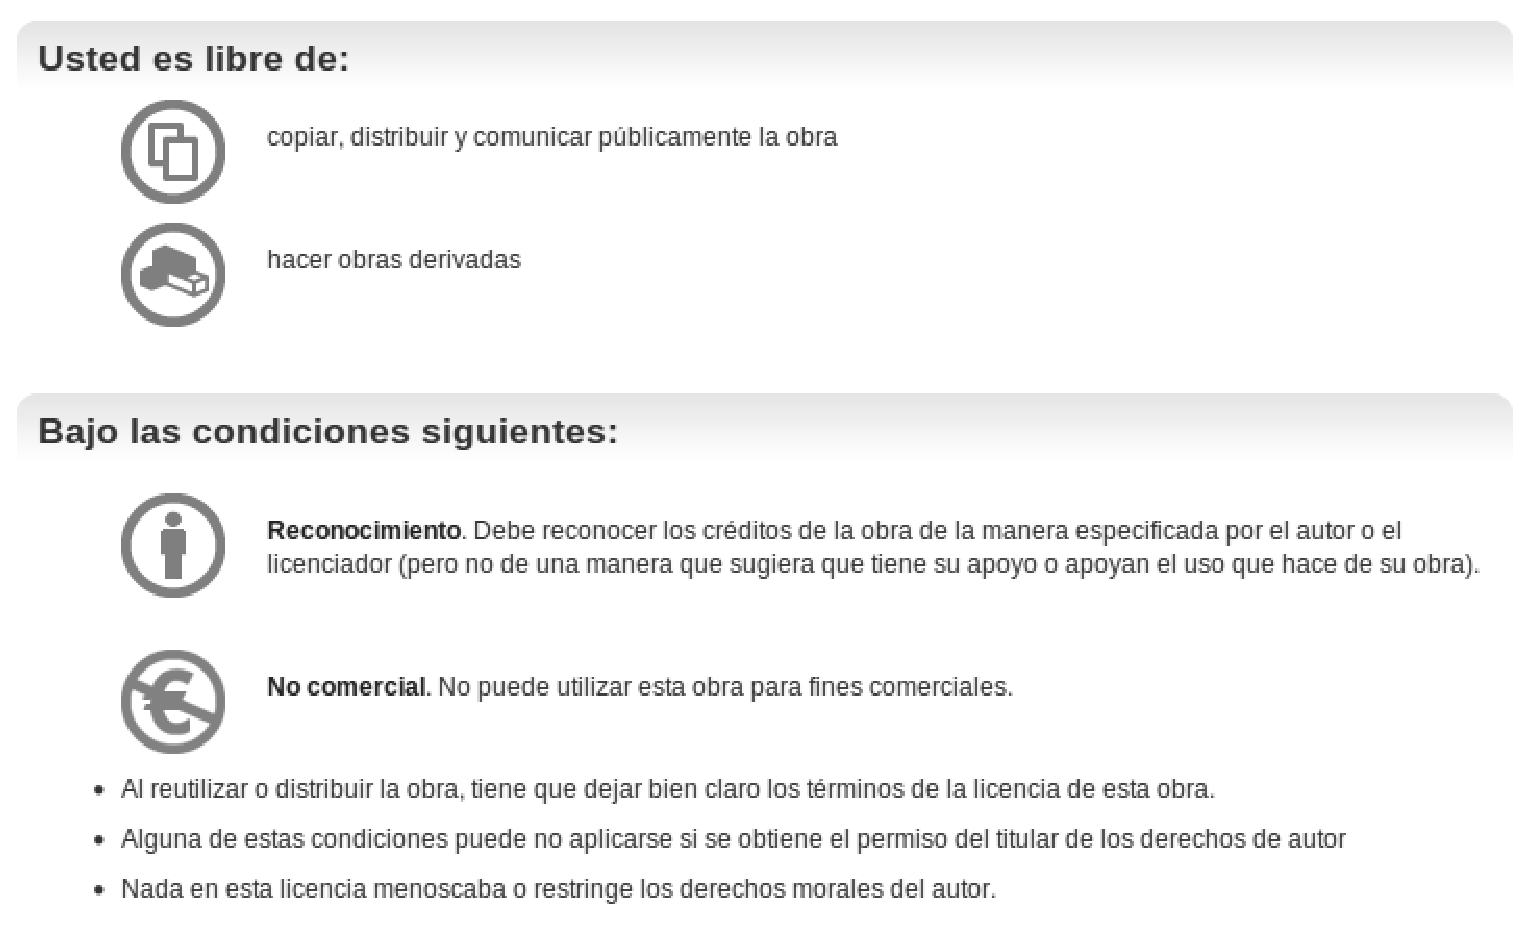
\includegraphics[width=1.1\textwidth]{licenciacc}
%\begin{tabular}{p{0.8cm} p{0.9\textwidth}}
\begin{tabular}{>{\centering\arraybackslash}m{0.8cm} >{\arraybackslash}p{0.9\textwidth}}
\multicolumn{2}{l}{\textbf{Usted es libre de:}}\\[0.5cm]
\includegraphics[width=0.8cm]{cc1.png} & Copiar, distribuir y comunicar p�blicamente la obra\\[0.5cm]
\includegraphics[width=0.8cm]{cc2.png} & Hacer obras derivadas\\[1cm]

\multicolumn{2}{l}{\textbf{Bajo las condiciones siguientes:}}\\[0.5cm]
\includegraphics[width=0.8cm]{cc3.png} & \textbf{Reconocimiento}. Debe reconocer los cr�ditos de la obra de la manera especificada por el autor o el licenciados (pero no de una manera que sugiera que tiene su apoyo o apoyan el uso que hace de su obra). \\[0.5cm]
\includegraphics[width=0.8cm]{cc4.png} & \textbf{No comercial}. No puede utilizar esta obra para fines comerciales.\\[0.5cm]
\end{tabular}
\begin{itemize}
\item Al reutilizar o distribuir la obra, tiene que dejar bien claro los t�rminos de la licencia de esta obra.
\item Alguna de estas condiciones puede no aplicarse si se obtiene el permiso del titular de los derechos de autor.
\item Nada en esta licencia menoscaba o restringe los derechos morales del autor.
\end{itemize}
\end{figure}

\noindent Puede consultar la licencia completa en: \\
\texttt{http://creativecommons.org/licenses/by-nc/3.0/es/legalcode.es}\\
\newline
\newline
Si ha encontrado alg�n error en el documento o desea contactar con el autor, puede hacerlo a trav�s de la siguiente direcci�n de email: \texttt{pmunoz@aut.uah.es}. Todos los comentarios ser�n bien recibidos.
\newpage

%--------------------------------------

%INDICES Y TABLAS
\setcounter{page}{1}
\pagenumbering{arabic}
\tableofcontents
\listoffigures
%\listoftables

%COMIENZO DEL DOCUMENTO
\chapter{Introducci�n}

Este documento representa una gu�a b�sica de uso y funcionamiento del lenguaje PLEXIL (\textit{Plan Execution Interchange Language}) para modelado de planes de alto nivel enfocados a sistemas aut�nomos y del ejecutor de planes dise�ado para �l: el \textit{Universal Executive} (en adelante UE).

PLEXIL fue originalmente desarrollado como un proyecto colaborativo entre investigadores de la NASA y de la Universidad Carnegie Mellon, bajo fondos del \textit{Mars Technology Program} a trav�s del \textit{Research Institute for Advanced Computer Science} (RIACS) en la \textit{Universities Space Research Association} (USRA). El proyecto comenz� en 2006 y actualmente esta en constante evoluci�n. Se encuentra bajo licencia BSD (\textit{Berkeley Software Distribution}) y se puede descargar el c�digo fuente completo con ficheros de ejemplo desde la p�gina del proyecto en SourceForge\cite{ref:plexuedesc}. Tambi�n puede consultarse en SourceForge la wiki del proyecto accediendo al enlace a trav�s de la p�gina de descarga del mismo.

PLEXIL y el UE han sido utilizados para demostraci�n integr�ndolo en el \textit{rover} K10 (figura \ref{fig:k10}) para pruebas de movilidad y de interacci�n hombre-robot. El K10 est� preparado para realizar tareas de inspecci�n. El programa desarrollado en el \textit{Ames Research Center} le permite realizar una inspecci�n completa de 360� a un SCOUT \textit{rover} tomando fotograf�as de alta resoluci�n en una serie de puntos predeterminados\cite{ref:k10}. Tambi�n ha sido probado en el \textit{Mars Drill}, un prototipo de taladro gestionado de forma aut�noma. Finalmente, se ha empleado para demostrar la automatizaci�n de algunas tareas en la Estaci�n Espacial Internacional (ISS).

\begin{figure}[h]
\begin{center}
 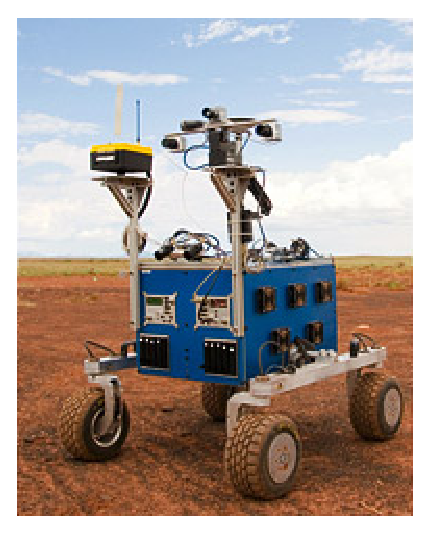
\includegraphics[width=3cm]{K10}
 \label{fig:k10}
 \caption{Robot K10}
\end{center}
\end{figure}

En �ste primer cap�tulo se dar� una descripci�n breve del lenguaje PLEXIL y el UE, as� como los elementos necesarios para poder utilizarlos y la instalaci�n de los mismos. En el segundo cap�tulo se abordar� el lenguaje PLEXIL, y en el tercero el funcionamiento del UE.


\section{Requisitos}

Las necesidades de los programas auxiliares de PLEXIL y el UE vienen descritas en el manual de PLEXIL\cite{ref:ueman} (este manual viene incluido en la distribuci�n de PLEXIL), habiendo sido probado correctamente en Red Hat Linux (versiones 4 y 5), MacOS X (10.4, 10.5 y 10.6) y Ubuntu\footnote{Para poder compilar \texttt{robosim} se deben tener instalados los siguientes paquetes: \texttt{glutg3, glutg3-dev, libxi-dev} y \texttt{libxmu-dev}} (desde la versi�n 8.04 hasta la 10.04), pero deber�a funcionar en la mayor�a de los sistemas basados en UNIX.

Para poder almacenar el c�digo fuente y los ejecutables es necesario disponer de al menos 150MB de espacio en disco. El uso de memoria RAM no est� calculado y depende de varios factores, no obstante, est� dise�ado con un enfoque eficiente para poder utilizarlo bajo sistemas empotrados con bajos recursos.

Tambi�n ser� necesario disponer de varios programas para poder compilar el c�digo y generar los correspondientes ejecutables para PLEXIL, el UE y otras herramientas de utilidad incluidas en la distribuci�n:
\begin{itemize}
	\item \textbf{g++}: el compilador de C++, versi�n 3.3.3 o superiores.\\(http://gcc.gnu.org)
	\item \textbf{ant}: herramienta para la automatizaci�n de la compilaci�n.\\(http://ant.apache.org/)
	\item \textbf{Java}: tanto la m�quina virtal de Java como el JDK (\textit{Java Development Kit}). Requiere la versi�n 1.5 o 1.6 (no se recomienda el uso de OpenJDK por carecer de un jar requerido).\\(http://www.java.com)
	\item \textbf{Doxygen}: herramienta opcional que permite generar autom�ticamente la documentaci�n del c�digo en varios formatos.\\(http://www.stack.nl/$\sim$dimitri/doxygen)
\end{itemize}


\section{Instalaci�n}

Una vez descargada la distribuci�n de plexil, habr� que realizar la compilaci�n del c�digo fuente. Para ello, primero habr� que descomprimir los archivos en una carpeta, en este caso usaremos \texttt{/home/usuario/plexil} como origen y despu�s ser� necesario definir la variable PLEXIL\_HOME y a�adir una nueva ruta al PATH de la \texttt{shell}. Ser� por tanto necesario modificar el archivo de inicio de la \texttt{shell} que utilicemos en nuestro sistema. Por ejemplo, para \texttt{bash} este archivo se ubicar� en \texttt{/home/usuario/.bashrc}. Para incluir las rutas necesarias ser� preciso insertar las l�neas que se indican en las figuras \ref{fig:varcsh} � \ref{fig:varbash} en el archivo correspondiente en funci�n del sistema usado.

\begin{figure}[!h]
\begin{center}
\begin{minipage}{12cm}
\lstset{language=c, breaklines=true, tabsize=3}
\lstset{commentstyle=\textit}
\lstset{stringstyle=\ttfamily, basicstyle=\footnotesize}
\begin{lstlisting}[frame=trbl]{}
setenv PLEXIL_HOME /home/usuario/plexil
setenv PATH $PLEXIL_HOME/bin:$PATH
(No Mac) setenv LD_LIBRARY_PATH $PLEXIL_HOME/lib
(s�lo Mac) setenv DYLD_LIBRARY_PATH $PLEXIL_HOME/lib
(s�lo Mac) setenv DYLD_BIND_AT_LAUNCH YES
\end{lstlisting}
\end{minipage}
\caption{Variables de entorno para \texttt{csh}}
\label{fig:varcsh}
\end{center}
\end{figure}

\begin{figure}[!h]
\begin{center}
\begin{minipage}{12cm}
\lstset{language=c, breaklines=true, tabsize=3}
\lstset{commentstyle=\textit}
\lstset{stringstyle=\ttfamily, basicstyle=\footnotesize}
\begin{lstlisting}[frame=trbl]{}
export PLEXIL_HOME=/home/usuario/plexil
export PATH=$PLEXIL_HOME/bin:$PATH
(No Mac) export LD_LIBRARY_PATH=$PLEXIL_HOME/lib
(s�lo Mac) export DYLD_LIBRARY_PATH=$PLEXIL_HOME/lib
(s�lo Mac) export DYLD_BIND_AT_LAUNCH=YES
\end{lstlisting}
\end{minipage}
\caption{Variables de entorno para \texttt{bash}}
\label{fig:varbash}
\end{center}
\end{figure}

Una vez definidas las variables en el archivo de configuraci�n de la \texttt{shell} se podr�n utiliar los ejecutables de PLEXIL y el UE desde cualquier directorio de forma c�moda, adem�s de poder emplear las librer�as din�micas de la distribuci�n en nuestros propios programas. Con esto realizado, habr� que situarse sobre el directorio de PLEXIL y ejecutar \texttt{make} para que de forma autom�tica compile y construya todos los elementos del sistema. El archivo \texttt{Makefile} s�lo ejecuta los correspondientes comandos que compilan cada elemento. Si se quiere realizar s�lo la compilaci�n de un elemento, basta con elegir la orden correspondiente. 

Cada objetivo del archivo construye un elemento\footnote{Durante la compilaci�n es posible que se den avisos por el uso de funciones obsoletas.}. \texttt{UniversalExec} construye el ejecutable del UE (cap�tulo \ref{cap:ue}), \texttt{luv} el visor gr�fico LUV (vease la secci�n \ref{sec:luv}), \texttt{standard-plexil} prepara el sistema de parseado y traducci�n para los planes de PLEXIL (m�s detalles en el cap�tulo \ref{cap:plexil}), y el resto de l�neas permiten generar herramienas auxiliares o simuladores de ejemplo incluidos en la distribuci�n.

La forma de ejecutar cada uno de los ejecutables generados se ver� posteriormente en sus respectivas secciones.

Una vez realizada la construcci�n de los elementos, se puede realizar la generaci�n de documentaci�n del c�digo. Para ello, basta con ejecutar las ordenes mostradas en la figura \ref{fig:docdoxy}. Con ello obtendremos la documentaci�n del c�digo en \texttt{\$PLEXIL\_HOME/src/exec/doc/index.html}.
\begin{figure}[!h]
\begin{center}
\begin{minipage}{12cm}
\lstset{language=c, breaklines=true, tabsize=3}
\lstset{commentstyle=\textit}
\lstset{stringstyle=\ttfamily, basicstyle=\footnotesize}
\begin{lstlisting}[frame=trbl]{}
cd $PLEXIL_HOME/src/exec
doxygen ue.dox
$
\end{lstlisting}
\end{minipage}
\caption{Generaci�n de la documentaci�n con Doxygen}
\label{fig:docdoxy}
\end{center}
\end{figure}


\subsection{Control de subversi�n}

PLEXIL est� mantenido en un sistema de control de subversiones (SVN). Mediante dicho sistema, tras la instalaci�n inicial de PLEXIL el usuario podr� interactuar con el SVN y actualizar los archivos de la distribuci�n a las �ltimas versiones. Para poder realizar las acciones que se detallan a continuaci�n, habr� que disponer del programa SVN en la m�quina local. Para obtener el programa puede dirigirse a su p�gina oficial:

\noindent \texttt{http://subversion.tigris.org/}.

El script \texttt{plexil/bin/checksvn} permitir� conocer si hay alguna versi�n nueva de los archivos en el repositorio SVN. Si se desea actualizar u obtener la �ltima versi�n disponible, basta con introducir la orden de la figura \ref{fig:svncheckout}.
\begin{figure}[!h]
\begin{center}
\begin{minipage}{12cm}
\lstset{language=bash, breaklines=true, tabsize=3}
\lstset{commentstyle=\textit}
\lstset{stringstyle=\ttfamily, basicstyle=\footnotesize}
\begin{lstlisting}[frame=trbl]{}
svn checkout https://plexil.svn.sourceforge.net/svnroot/plexil/trunk plexil
\end{lstlisting}
\end{minipage}
\caption{Obtenci�n de la �ltima versi�n de PLEXIL}
\label{fig:svncheckout}
\end{center}
\end{figure}

Con ello obtendremos una copia actualizada (o actualizaremos la copia local) de todos los componentes de PLEXIL. La copia se albergar� en una carpeta de nombre \texttt{plexil} en el directorio desde el cual ejecutemos la orden. Si desea conocer m�s acerca de SVN puede consultar \cite{ref:svn}.
\chapter{El lenguaje PLEXIL}\label{cap:plexil}

En este cap�tulo se ver�n los elementos que conforman el lenguaje de ejecuci�n PLEXIL y la codificaci�n de los mismos, adem�s de como llevar a cabo la traducci�n de los planes escritos en las diferentes versiones del lenguaje PLEXIL a XML mediante las herramientas desarrolladas a tal efecto. Adem�s se ver� la codificaci�n de PlexilScript, con el cual podremos realizar simulaciones de planes mediante la aplicaci�n TestExec que se ver� en el cap�tulo \ref{cap:ue}.


\section{Introducci�n a PLEXIL}

PLEXIL es un lenguaje para el modelado y representaci�n de planes de ejecuci�n de sistemas aut�nomos. Es v�lido tanto para sistemas mono-agente como para multi-agente ya sea en entornos reales o simulados. Est� dise�ado de tal forma que sea compacto, sem�nticamente sencillo y determinista siempre que se de la misma secuencia de sucesos en el mundo exterior. A pesar de ser un lenguaje sencillo, permite definir bucles, condiciones de salto, actividades basadas en tiempo y eventos, actividades concurrentes o en secuencia y permite restricciones temporales y manejo de recursos. El n�cleo de la sintaxis es simple y uniforme, lo que permite una f�cil y r�pida interpretaci�n de los planes escritos por parte del planificador.

Hay que destacar que PLEXIL, al contrario que otros lenguajes de planificaci�n como, por ejemplo, PDDL\cite{ref:pddl}, tiene una �nica entrada, es decir, el plan y el problema son un �nico elemento. Esto es as� ya que un plan de PLEXIL consta de una serie de elementos de acci�n que podr�n ser o no ejecutados en funci�n del estado del mundo, la ejecuci�n correcta o no de otras acciones y, a su vez, estas acciones constituyen metas que deben ser alcanzadas. El plan finalizar� una vez todas las posibles acciones que se puedan ejecutar, hayan sido ejecutadas (independientemente del resultado de la ejecuci�n). Estos elementos de ejecuci�n son los nodos.

El formato de lenguaje PLEXIL ser� XML, aunque la codificaci�n de los planes podr� realizarse de dos formas: utilizando el lenguaje PLEXIL est�ndar (en adelante Plexil) o PlexilLisp. La codificaci�n que se ver� en las siguientes secciones corresponde al lenguaje PLEXIL est�ndar. Con estos planes escritos, mediante un programa creado para ello, se realizar� el an�lisis sint�ctico y sem�ntico del mismo y se encargar� de realizar la traducci�n al formato XML. El archivo XML generado ser� el que utilizar� el ejecutor como elemento de entrada.

%SALTO DE PAGINA
\newpage
\section{Nodos}

Los nodos son el elemento fundamental del lenguaje PLEXIL. Todo plan escrito en PLEXIL constar� de uno o m�s nodos. Cada nodo a su vez constar� de dos elementos:
\begin{itemize}
    \item \textbf{Condiciones}: una serie de condiciones que permitir�n controlar cuando puede ejecutarse el cuerpo del nodo, que ha de ocurrir para que finalice correctamente o cuando puede volver a ser apto para ejecuci�n por ejemplo. Todas las posibles condiciones se ver�n en la secci�n \ref{sec:condiciones}.
    \item \textbf{Cuerpo}: el cuerpo del nodo determina las acciones que llevar� a cabo el nodo. En funci�n de la acci�n que ejecute el nodo se considerar� un tipo u otro de nodo. Por ejemplo, existen nodos de asignaci�n, de comando o de llamada a funci�n. Los tipos de nodos y sus particularidades se ver�n en la secci�n \ref{sec:tipos}.
\end{itemize}

Un plan de PLEXIL ser� un �rbol de nodos que representar� una descomposici�n jer�rquica de tareas que debe llevar a cabo el plan. En este sentido, lo normal ser� distribuir las tareas de tal forma que las de m�s alto nivel se sit�en cercanas a la ra�z del �rbol y las de menor nivel se aproximen a las hojas. El n�mero de ramas y la profundidad del �rbol la determinaremos a la hora de escribir el plan en funci�n de nuestras necesidades. En la figura \ref{fig:arbol} puede verse gr�ficamente un plan de ejemplo.

\begin{figure}[h]
\begin{center}
 \includegraphics[width=12cm]{planej}
 \caption{Ejemplo gr�fico de un plan escrito en PLEXIL}
 \label{fig:arbol}
\end{center}
\end{figure}

En las siguientes subsecciones veremos como se declara un nodo y los atributos que pueden utilizarse dentro del lenguaje. Tras ello, se analizar�n las siete condiciones posibles que se pueden utilizar para controlar la ejecuci�n de los nodos y los seis tipos de nodos disponibles en PLEXIL.

\subsection{Declaraci�n}

Para declarar un nodo en lenguaje Plexil se recurre a la estructura mostrada en la figura \ref{fig:decnodo}. En la declaraci�n, \textit{nombre} representa la identificaci�n un�voca del nodo. Los datos del nodo ser�n variables, condiciones de ejecuci�n y los datos propios del nodo en funci�n del tipo de nodo que sea (las variables y condiciones son opcionales). El tipo de nodo no es necesario declararlo, ya que ser� determinado autom�ticamente en funci�n de los datos que se introduzcan en �l.

\begin{figure}[!h]
\begin{center}
\begin{minipage}{12cm}
\lstset{language=c++, breaklines=true, tabsize=3}
\lstset{commentstyle=\textit}
\lstset{stringstyle=\ttfamily, basicstyle=\footnotesize}
\begin{lstlisting}[frame=trbl]{}
nombre:
{
   <datos>
}
\end{lstlisting}
\end{minipage}
\caption{Declaraci�n de un nodo en Plexil}
\label{fig:decnodo}
\end{center}
\end{figure}

Un nodo puede no estar nombrado, en cuyo caso ser� �nicamente un par de corchetes en cuyo interior estar� el cuerpo del nodo. Aunque esto es v�lido, no suele ser pr�ctico ya que no puede referenciarse de ninguna manera al nodo.


\section{Variables}

En Plexil se pueden declarar variables locales dentro de un nodo. Existen cuatro tipo de variables: \texttt{Boolean, Integer, Real} y \texttt{String}. Adem�s se podr�n declarar vectores para cada tipo simple. Hay que indicar que s�lo existen variables, no se pueden declarar constantes como tal.

Los variables se declaran como sigue: \texttt{tipo nombre = valor;} donde la asignaci�n inicial puede omitirse, tomando entonces \texttt{UNKNOWN} como valor la variable declarada. En la figura \ref{fig:vars} pueden verse varios ejemplos de declaraci�n de variables.

\begin{figure}[!h]
\begin{center}
\begin{minipage}{12cm}
\lstset{language=c++, breaklines=true, tabsize=3}
\lstset{commentstyle=\textit}
\lstset{stringstyle=\ttfamily, basicstyle=\footnotesize}
\begin{lstlisting}[frame=trbl]{}
Boolean iniciar = true;
Integer pasos;
Real pi = 3.141592;
String mensaje = "Inicializado";
\end{lstlisting}
\end{minipage}
\caption{Ejemplos de declaraci�n de variables}
\label{fig:vars}
\end{center}
\end{figure}

Como se ha indicado, para cada uno de los cuatro tipos simples, se pueden declarar vectores o arrays unidimensionales. Se declaran de la siguiente forma: \texttt{tipo nombre[dimensi�n] = \#(val1 val2 ...);}, debiendo siempre especificarse la dimensi�n del mismo. Para trabajar con los arrays hay que trabajar con cada elemento independientemente referenciado por su posici�n (\texttt{array[pos]}), no pudiendo trabajar con el array completo. En la figura \ref{fig:arrays} pueden verse ejemplos de declaraci�n de arrays. Los arrays al igual que las variables simples se inicializar�n a \texttt{UNKNOWN} en caso de no especificar los valores, salvo que en el caso de los arrays pueden especificarse los primeros n valores, dejando el resto indeterminados. Es importante destacar que los arrays comienzan en la posici�n 0.
\begin{figure}[!h]
\begin{center}
\begin{minipage}{12cm}
\lstset{language=c++, breaklines=true, tabsize=3}
\lstset{commentstyle=\textit}
\lstset{stringstyle=\ttfamily, basicstyle=\footnotesize}
\begin{lstlisting}[frame=trbl]{}
Integer temperaturas[100];
Real predefinido[10] = #(1.3 2.0 3.5);
Integer X[6] = [1,3,5];
\end{lstlisting}
\end{minipage}
\caption{Ejemplos de declaraci�n de arrays}
\label{fig:arrays}
\end{center}
\end{figure}


\subsection{Visibilidad de variables}

Las variables ser�n visibles localmente por el nodo que las haya declarado en su cuerpo y por todos sus hijos. Este es el comportamiento general y se puede modificar explicitamente mediante el empleo de clausulas de interfaz. Estas clausulas definir�n los variables que ser�n accesibles a los hijos del nodo que las declara y la forma en que estos pueden acceder. Si se ha declarado la interfaz para al menos una variable en el nodo, el resto de variables cuya interfaz no sea declarada se asumir� directamente que son inaccesibles a los hijos. Las dos clausulas de interfaz son las siguientes:

\begin{itemize}
	\item \texttt{In}: esta clausula permite que los hijos lean las variables. Una variable de lectura no podr� ser redeclarada por un hijo como lectura y escritura.
	\item \texttt{InOut}: permite la lectura y escritura de la variable por los nodos hijos.
\end{itemize}
\begin{figure}[!h]
\begin{center}
\begin{minipage}{12cm}
\lstset{language=c++, breaklines=true, tabsize=3}
\lstset{commentstyle=\textit}
\lstset{stringstyle=\ttfamily, basicstyle=\footnotesize}
\begin{lstlisting}[frame=trbl]{}
Interfaz:
{
  In x, y;
  InOut z;
  Integer a, b;
}
\end{lstlisting}
\end{minipage}
\caption{Ejemplo de interfaces}
\label{fig:interfaz}
\end{center}
\end{figure}

En la figura \ref{fig:interfaz} puede verse un ejemplo de un nodo con una serie de variables. En dicho nodo, las variables \textit{x} e \textit{y} ser�n accesibles a sus descendientes como variables de s�lo lectura, mientras que \textit{z} lo ser� para lectura y escritura. Finalmente, las variables \textit{a} y \textit{b}, al no tener una interfaz declarada, no ser�n accesibles por los nodos hijos.


\subsection{Expresiones}

A la hora de actuar con variables se recurre a las expresiones. La forma de estas expresiones depender� del tipo de variables sobre el que trabajen, pero una expresi�n en PLEXIL ser� esencialmente un valor literal, una variable, una consulta al estado del mundo exterior, el valor de un estado de un nodo, o una combinaci�n de estos elementos. Por tanto, una expresi�n puede contener expresiones combinadas entre ella mediante el uso de operadores.

Adem�s de aparecer para la asignaci�n de variables, las expresiones podr�n aparecer en las condiciones que gestionan la ejecuci�n de los nodos o en la gesti�n de recursos.

Para el caso de operaciones num�ricas, se podr� recurrir a los operadores tradicionales: suma, resta, multiplicaci�n y divisi�n, as� como a ra�ces cuadradas\footnote{Si se intenta obtener la ra�z de un n�mero negativo (resultado complejo) se producir� un error en la ejecuci�n.} (\texttt{sqrt}) y valor absoluto\footnote{Aunque el valor absoluto est� definido, no es as� para el negativo, el signo '-' s�lo es v�lido como resta, no se permite como inversor de signo. Para obtener el negativo a partir de un n�mero positivo, se deber� recurrir a la expresi�n (0-x).} (\texttt{abs}). Ser� posible en algunos casos mezclar n�meros reales y n�meros enteros siendo el tipo resultante dependiente del contexto\footnote{Estos casos no est�n documentados, aunque son intuitivos.}. Las reglas de precedencia y asociaci�n de operadores son las reglas est�ndar, permiti�ndose el uso de par�ntesis para especificar el orden de operaci�n. En la figura \ref{fig:opnum} se pueden ver ejemplos de expresiones num�ricas.
\begin{figure}[!h]
\begin{center}
\begin{minipage}{12cm}
\lstset{language=c++, breaklines=true, tabsize=3}
\lstset{commentstyle=\textit}
\lstset{stringstyle=\ttfamily, basicstyle=\footnotesize}
\begin{lstlisting}[frame=trbl]{}
resultado = numreal / 14.5;
x1 = -b + (sqrt(b*b - 4*a*c) / (2*a));
tempVal = (temperatura[2] - 32) * 5 / 9;
absoluto = abs(real);
\end{lstlisting}
\end{minipage}
\caption{Ejemplos de expresiones num�ricas}
\label{fig:opnum}
\end{center}
\end{figure}

Las expresiones l�gicas vendr�n determinadas por los operadores de comparaci�n (igualdad: \texttt{==}, desigualdad: \texttt{!=}, mayor que o mayor o igual que: \texttt{>\ o >=} y menor que o menor o igual que: \texttt{<\ o <=}) o los operadores l�gicos (negaci�n: \texttt{!}, disyunci�n u OR: \texttt{$\Vert$}, conjunci�n o AND: \texttt{\&\&} y disyunci�n exclusiva o XOR: \texttt{XOR}). Con estos operadores se podr�n formar expresiones cuyo resultado ser� siempre un valor l�gico (consulte la secci�n \ref{sec:logica} para conocer los valores l�gicos posibles). En la figura \ref{fig:oplog} pueden verse ejemplos de expresiones l�gicas.
\begin{figure}[!h]
\begin{center}
\begin{minipage}{12cm}
\lstset{language=c++, breaklines=true, tabsize=3}
\lstset{commentstyle=\textit}
\lstset{stringstyle=\ttfamily, basicstyle=\footnotesize}
\begin{lstlisting}[frame=trbl]{}
enmovimiento = velocidad > 0;
estado = reconocido && !(contador <= 30);
conocido = isKnown(valor);
\end{lstlisting}
\end{minipage}
\caption{Ejemplos de expresiones l�gicas}
\label{fig:oplog}
\end{center}
\end{figure}

Para las cadenas de caracteres se permite s�lo el paso de �stas como par�metros. la concatenaci�n (\texttt{+}) y la comparaci�n de igualdad (\texttt{==}) o desigualdad (\texttt{!=}) entre cadenas. En la figura \ref{fig:opcad} se pueden ver ejemplos de operaci�n con cadenas de caracteres.
\begin{figure}[!h]
\begin{center}
\begin{minipage}{12cm}
\lstset{language=c++, breaklines=true, tabsize=3}
\lstset{commentstyle=\textit}
\lstset{stringstyle=\ttfamily, basicstyle=\footnotesize}
\begin{lstlisting}[frame=trbl]{}
mensaje = "Bienvenido ";
entrada = mensaje + "usuario";
\end{lstlisting}
\end{minipage}
\caption{Ejemplos de expresiones con cadenas}
\label{fig:opcad}
\end{center}
\end{figure}

Finalmente, se podr� operar con los elementos del array, y nunca con el array completo. Para operar con un elemento del array habr� que extraerlo mediante el operador \texttt{[i]}, donde \texttt{i} es el �ndice, comprendido entre 0 y el tama�o m�ximo del array. Para asignar el valor a un elemento del array se referenciar� al elemento de la misma manera. Adem�s es posible asignar un array a otro, de tal manera que si el array de destino es mayor que el origen, los elementos restantes obtendr�n el valor \texttt{UNKNOWN}. En caso de que el array destino fuera menor que el origen se producir�a un error. En la figura \ref{fig:oparr} se puden ver varios ejemplos de manipulaci�n de arrays.
\begin{figure}[!h]
\begin{center}
\begin{minipage}{12cm}
\lstset{language=c++, breaklines=true, tabsize=3}
\lstset{commentstyle=\textit}
\lstset{stringstyle=\ttfamily, basicstyle=\footnotesize}
\begin{lstlisting}[frame=trbl]{}
Integer numeros[9];
Integer X[6] = [1,3,5];
numeros[8] = 9;
X[5] = numeros[8] * X[2];
numeros = X;
\end{lstlisting}
\end{minipage}
\caption{Ejemplos de expresiones con arrays}
\label{fig:oparr}
\end{center}
\end{figure}

A continuaci�n se describen varias operaciones que no admiten el uso de arrays:
\begin{itemize}
	\item Un array como valor de retorno de un comando o llamada a funci�n.
	\item Arrays completos como parte de una expresi�n (salvo asignaci�n a otro array).
	\item Arrays enteros como par�metro de una funci�n (s�lo se permiten elementos).
	\item Arrays como variables dentro de una interfaz.
\end{itemize}

PLEXIL implementa un tipo de expresiones para el tiempo y la duraci�n (\textit{Date and Duration expressions}) que son definidas bajo el est�ndar ISO-8601 \cite{ref:iso8601}. Este tipo de expresiones est�n pensadas para el uso de operaciones temporales para \textit{lookups} y actividades que requieran referencias de tiempo real. Permiten a su vez el uso de operaciones aritm�ticas como las vistas anteriormente.

\begin{figure}[!h]
\begin{center}
\begin{minipage}{12cm}
\lstset{language=c++, breaklines=true, tabsize=3}
\lstset{commentstyle=\textit}
\lstset{stringstyle=\ttfamily, basicstyle=\footnotesize}
\begin{lstlisting}[frame=trbl]{}
// Tiempo UTC
Date fecha1 = Date("2013-12-12T09:43:00.00Z"); 

// Hora local
Date fecha2 = "2013-15-03T20:32:00.00";	

// Duraci�n de 45 minutos
Duration dur1 = Duration("PT45M");

// Ejemplo de operaciones
Date fecha3;
Duration dur2;

// Resta de 3.2 segundos a la fecha1
fecha3 = fecha1 - Duration("PT3.2S"); 

// Resta de 2 minutos a la fecha2
dur2 = fecha2 - Date("2013-15-03T20:30:00.00");

\end{lstlisting}
\end{minipage}
\caption{Ejemplos de expresiones de tiempo y duraci�n}
\label{fig:datedur}
\end{center}
\end{figure}

\subsection{L�gica trivaluada y el valor \texttt{UNKNOWN}}\label{sec:logica}

En PLEXIL se utiliza una l�gica de tres valores, en la cual a los valores t�picos de las l�gicas bivaluadas (\texttt{true} y \texttt{false}) se le a�ade el valor \texttt{UNKNOWN}. Por tanto, los operadores l�gicos se han redefinido para operar con este valor como se ve en la figura \ref{fig:trival}.

\begin{figure}[!h]
\begin{center}
\begin{minipage}{12cm}
\lstset{language=pascal, breaklines=true, tabsize=3}
\lstset{commentstyle=\textit}
\lstset{stringstyle=\ttfamily, basicstyle=\footnotesize}
\begin{lstlisting}[frame=trbl]{}
True    && UNKNOWN = UNKNOWN
False   && UNKNOWN = False
True    || UNKNOWN = True
False   || UNKNOWN = UNKNOWN
UNKNOWN && UNKNOWN = UNKNOWN
UNKNOWN || UNKNOWN = UNKNOWN
         ! UNKNOWN = UNKNOWN
\end{lstlisting}
\end{minipage}
\caption{Operadores l�gicos y el valor \texttt{UNKNOWN}}
\label{fig:trival}
\end{center}
\end{figure}

Adem�s, como ya se indic�, el valor \texttt{UNKNOWN} puede aparecer como valor de cualquier tipo de variable, y, por tanto, puede ser resultado de una expresi�n. Esto �ltimo ocurrir� en los siguientes casos:
\begin{itemize}
	\item Aparece como valor inicial de una variable (ya sea simple o elementos de un array) por no haber declarado el valor inicial.
	\item Es el estado final inicial de un nodo.
	\item Como resultado de una consulta al estado del mundo fallida.
	\item Como resultado de consultar acerca de un evento temporal que no ha ocurrido.
\end{itemize}

Este valor no aparece de forma literal, es decir, no se puede asignar de forma directa y solo aparece por las condiciones expuestas anteriormente. No obstante, mediante el empleo de la funci�n \texttt{isKnown(\textit{variable})} se puede comprobar este valor. Si la funci�n retorna \texttt{false}, entonces el argumento se puede evaluar a \texttt{UNKNOWN} y, en caso contrario, retornar� \texttt{true}.


\section{Condiciones}\label{sec:condiciones}
Para el control de la ejecuci�n de cada nodo al inicio, fin o durante, se pueden definir hasta siete condiciones. Cada condici�n ir� seguida de una expresi�n booleana: \texttt{tipo\_condicion <expresi�n\_booleana>;}. Estas siete condiciones se enmarcar�n en dos grupos: las \textit{gate conditions}, que comprende las condiciones de inicio, finalizaci�n, repetici�n y omisi�n, y el grupo denominado \textit{check conditions}, dentro del cual est�n las precondiciones, postcondiciones y condiciones invariables. El primer grupo determinar� cuando el nodo puede comenzar o finalizar su ejecuci�n y el segundo grupo permite determinar condiciones por las cuales la ejecuci�n del nodo no fue correcta. En la figura \ref{fig:ejcondiciones} puede verse un ejemplo de un nodo con todas las condiciones definidas.

A la hora de trabajar con las condiciones ser� muy �til (y necesario en muchos casos) permitir o no la ejecuci�n de un nodo en funci�n del resultado de la ejecuci�n de otro. Para ello se podr�n utilizar los estados de los nodos (ve�se la secci�n \ref{sec:estados}) en las condiciones.
\begin{figure}[!h]
\begin{center}
\begin{minipage}{12cm}
\lstset{language=c++, breaklines=true, tabsize=3}
\lstset{commentstyle=\textit}
\lstset{stringstyle=\ttfamily, basicstyle=\footnotesize}
\begin{lstlisting}[frame=trbl]{}
subir_temperatura:
{
	StartCondition temperaturaBaja;
	EndCondition temperatura >= 20 || isKnow(temperatura);
	RepeatCondition temperatura < 20;
	SkipCondition temperatura > 20 || !temperaturaBaja;
	PreCondition temperatura > -10 && temperatura <30;
	PostCondition temperatura > -10;
	InvariantCondition !temperaturaBaja;
	Command: temperatura = SubirTemp(incremento);
}
\end{lstlisting}
\end{minipage}
\caption{Ejemplo de nodo con todas las condiciones}
\label{fig:ejcondiciones}
\end{center}
\end{figure}

\subsection{Condici�n de inicio, \textit{StartCondition}}

Esta condici�n indica cuando el nodo puede comenzar a ejecutarse. En el momento que la condici�n indicada se cumpla, �ste comenzar� su ejecuci�n. En caso de no haber, el nodo iniciar� la ejecuci�n en el momento que la ejecuci�n del plan alcance el nivel de profundidad del nodo en cuesti�n.

\subsection{Condici�n de finalizaci�n, \textit{EndCondition}}

Indica la condici�n para que el nodo termine su ejecuci�n. En caso de omitirse, el nodo terminar� la ejecuci�n una vez haya realizado la acci�n de su cuerpo.

\subsection{Condici�n de repetici�n, \textit{RepeatCondition}}

Esta condici�n permite que un nodo que ya ha sido ejecutado vuelva a ser apto para ejecutarse. Para ello, el nodo en cuesti�n deber� cumplir con la condici�n de repetici�n y la condici�n de inicio y precondici�n en caso de tenerlas. Hay que tener en cuenta que un nodo que ya ha sido ejecutado (correcta o incorrectamente) no se volver� a ejecutar salvo que se indique una condici�n de repetici�n.

\subsection{Condici�n de omisi�n, \textit{SkipCondition}}

La condici�n de omisi�n permite establecer un nodo como ejecutado por omisi�n (que implica que el nodo haya finalizado su ejecuci�n). En caso de que un nodo posea esta condici�n y se verifique en el momento en que pueda entrar en ejecuci�n, el nodo no ser� ejecutado. Esta condici�n permite definir saltos del tipo \texttt{if-then-else} combin�ndola con otras condiciones.

\subsection{Precondici�n, \textit{PreCondition}}

Esta condici�n se eval�a despu�s de la condici�n de inicio y determina si es seguro proceder a la ejecuci�n del nodo. Para que un nodo pueda ejecutarse, deber� verificar primero la condici�n de inicio y luego la precondici�n. En caso de no cumplir la precondici�n, el nodo no podr� ejecutarse y ser� abortado indicando que la ejecuci�n ha sido fallida.

\subsection{Postcondici�n, \textit{PostCondition}}

La postcondici�n se eval�a tras la ejecuci�n del nodos y despu�s de evaluar la condici�n de finalizaci�n. Esta condici�n permite comprobar si el nodo ha realizado su funci�n correctamente. Si la condici�n especificada no se cumple, el nodo no habr� cumplido con sus objetivos y se marcar� como fallido.

\subsection{Condici�n invariable, \textit{InvariantCondition}}

Esta condici�n ser� comprobada durante toda la ejecuci�n del nodo de tal forma que deber� cumplirse en todo momento. Si en el transcurso de la ejecuci�n se da alguna circunstancia que implique que la condici�n invariable no se cumpla, se abortar� la ejecuci�n del nodo y se marcar� como fallido. Es una condici�n �til para determinar las condiciones de seguridad en las cuales debe ejecutarse el nodo.


\subsection{Jerarqu�a de condiciones}

Las condiciones se pueden agrupar en una jerarqu�a en base al control de inicio, ejecuci�n y finalizaci�n del nodo. Esta jerarqu�a puede verse en la figura \ref{fig:jcond} y es como sigue:
\begin{itemize}
	\item \textbf{Inicio del nodo}: la primera condici�n que se verificar� es la condici�n de omisi�n, s�lo si �sta se verifica podr�n comprobarse el resto, sino se omitir� el nodo. Despu�s se comprobar� la condici�n de inicio, no comprob�ndose el resto hasta que esta no se satisfaga. Una vez comprobada esta condici�n, se podr� ver si se cumple la precondici�n, y, en caso de cumplirse, se ejecutar� el nodo. Si la precondici�n no se cumple, el nodo finalizar� por fallo en la precondici�n. En caso de que el nodo disponga de una condici�n de repetici�n, ser� la �ltima en comprobarse siempre que el nodo ya se haya ejecutado al menos una vez.
	\item \textbf{Ejecuci�n del nodo}: durante la ejecuci�n del nodo se comprobar� la condici�n invariante. Est� deber� verificarse durante todo el per�odo de ejecuci�n del nodo, provocando el aborto de la ejecuci�n en caso de no cumplirse. En dicho caso, lo indicar� mediante un fallo en la condici�n invariante.
	\item \textbf{Finalizaci�n del nodo}: una vez ejecutado el nodo, se comprobar� la condici�n de finalizaci�n. En caso de cumplirse, ser� comprobada la postcondici�n. Hasta que no se verifique la condici�n de finalizaci�n el nodo seguir� en estado de ejecuci�n. Si la condici�n de finalizaci�n es correcta, pero la postcondici�n no, el nodo finalizar� con un fallo por la postcondici�n.\\
\end{itemize}

\begin{figure}[h]
\begin{center}
 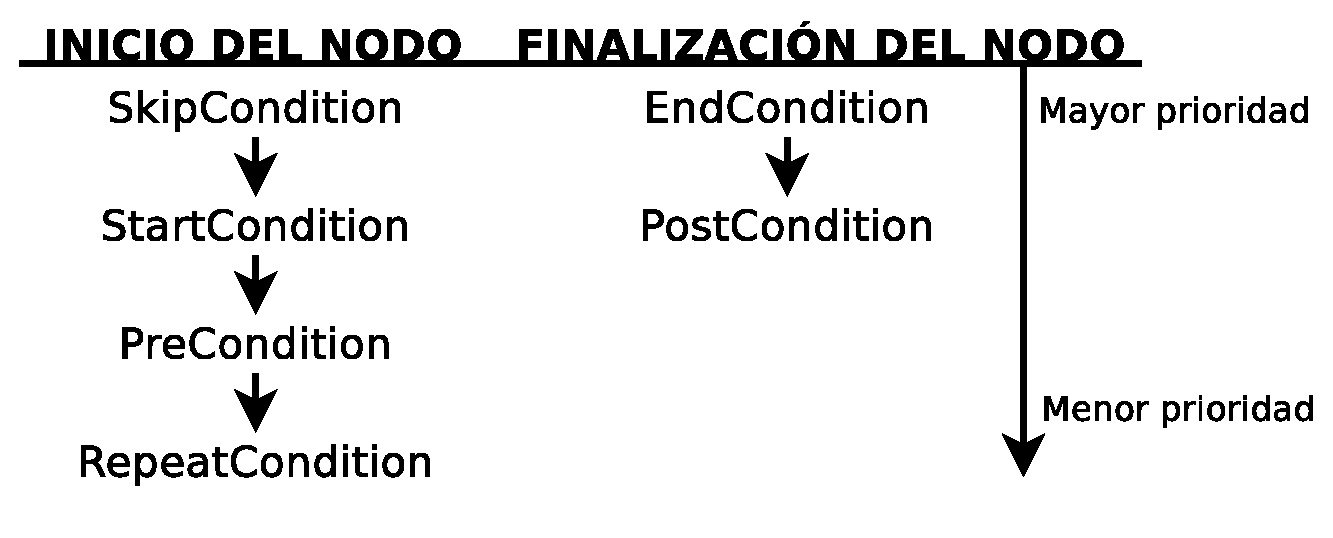
\includegraphics[width=10cm]{condiciones}
 \caption{Jerarqu�a de condiciones}
 \label{fig:jcond}
\end{center}
\end{figure}


\section{Tipos de nodos}\label{sec:tipos}

En esta secci�n se describir�n los seis\footnote{Existe un s�ptimo tipo de nodo, el nodo de solicitud de planificaci�n (\textit{Plan Request node}), que est� dise�ado y parcialmente implementado. Este nodo soporta interacci�n con planificadores externos permitiendo un punto de enganche para a�adir un nuevo plan. En este momento este tipo no esta soportado oficialmente por PLEXIL ni es plenamente funcional.} tipos de nodos existentes en PLEXIL. Como ya se dijo anteriormente, los nodos se estructuran como un �rbol. En este sentido, se conservar�n las definiciones cl�sicas: el nodo superior en la jerarqu�a ser� la ra�z, siendo un nodo \textit{lista} del cual colgar�n m�s nodos que pueden ser hojas (nodos de cualquier tipo que no sea lista) u otro nodo lista que generar� otro nivel de profunidad en el �rbol. Ser� importante la distinci�n entre nodo padre e hijo: un nodo padre ser� un nodo lista y los hijos los nodos inmediatamente inferiores que dependan de dicho nodo. Por tanto, un nodo lista ser� siempre un nodo interior y cualquier otro tipo de nodo ser� un nodo hoja e hijo de un nodo lista. Ser�n estos nodos hojas los encargados de interactuar con el mundo y realizar las acciones pertientes del plan.

A continuaci�n se analizar�n los seis tipos de nodos. Aqu� se ver�n los elementos que conforman parte del cuerpo del nodo para cada tipo particular.

\subsection{Nodo vac�o, \textit{Empty node}}

Un nodo vac�o es aquel que no realiza ninguna acci�n. Estos nodos s�lo pueden contener atributos y en la pr�ctica son poco comunes y su utilidad suele ser verificar el estado del mundo exterior. En este sentido tendr� alguna condici�n que permita realizar una comprobaci�n y, en base a ello, generar un estado de salida del nodo que sea �til para la ejecuci�n de otro nodo.
\begin{figure}[!h]
\begin{center}
\begin{minipage}{12cm}
\lstset{language=c++, breaklines=true, tabsize=3}
\lstset{commentstyle=\textit}
\lstset{stringstyle=\ttfamily, basicstyle=\footnotesize}
\begin{lstlisting}[frame=trbl]{}
ExcesoTemp:
{
	PostCondition LookupNow("temperatura") > 100.0;
}
\end{lstlisting}
\end{minipage}
\caption{Ejemplo de nodo vac�o}
\label{fig:nvacio}
\end{center}
\end{figure}


\subsection{Nodo de asignaci�n, \textit{Assignment node}}

Un nodo de asignaci�n permite modificar el estado de una variable mediante una expresi�n l�gica o matem�tica. En el lado izquierdo de la expresi�n deber� haber una variable apta para escritura y en el lado derecho una expresi�n. Esta expresi�n constar� de, al menos, un operando o literal (en caso de una asignaci�n simple) o dos operandos unidos por un operador. En todos los casos, el resultado de la expresi�n debe ser del mismo tipo que la variable a la cual se asignar� el resultado. Los operandos pueden ser una varible simple, un elemento de un array (nunca un array completo) o un literal. Dentro de la expresi�n se pueden utilizar par�ntesis para priorizar los c�lculos. La clausula de asignaci�n y un ejemplo de nodo de asignaci�n se pueden ver en la figura \ref{fig:nasignacion}. S�lo podr� haber una clausula de asignaci�n por nodo con una �nica asignaci�n. En actuales revisiones de PLEXIL, se permite la omisi�n del \textit{tag} \texttt{Assignment:}.

\begin{figure}[!h]
\begin{center}
\begin{minipage}{12cm}
\lstset{language=c++, breaklines=true, tabsize=3}
\lstset{commentstyle=\textit}
\lstset{stringstyle=\ttfamily, basicstyle=\footnotesize}
\begin{lstlisting}[frame=trbl]{}
Assignment: <variable> = <expresion>;

incrementarAngulo:
{
	Assignment: angulo = angulo + 25;
}

convertirTempSens2
{
	Assignment: temperatura = (sensorTemp[2] - 32) * 5 / 9;
}
\end{lstlisting}
\end{minipage}
\caption{Clausula de asignaci�n y ejemplos}
\label{fig:nasignacion}
\end{center}
\end{figure}


\subsection{Nodo de comando, \textit{Command node}}

Los nodos de comando permiten ejecutar acciones soportadas e implementadas en el sistema a controlar. El funcionamiento de estos nodos ser� llamar a una funci�n externa con los par�metros adecuados. Estos par�metros ser� una lista formada por literales o variables, pero nunca por expresiones. Adem�s, si la funci�n implementada retorna un valor de un tipo reconocido por PLEXIL, podr� ser asignado a una variable. En la figura \ref{fig:ncomando} puede verse la clausula que determina al nodo de comando. �sta especifica el nombre del comando a ejecutar seguido por la lista de par�metros que utilizar� entre par�ntesis. La lista de par�metros estar� separada por comas y ser� opcional. En caso de querer asignar el valor resultante a una variable, bastar� con indicarlo mediante la asignaci�n correspondiente, siempre y cuando sea posible escribir en dicha variable desde el nodo. En actuales revisiones de PLEXIL, se permite la omisi�n del \textit{tag} \texttt{Command:}.

\begin{figure}[!h]
\begin{center}
\begin{minipage}{12cm}
\lstset{language=c++, breaklines=true, tabsize=3}
\lstset{commentstyle=\textit}
\lstset{stringstyle=\ttfamily, basicstyle=\footnotesize}
\begin{lstlisting}[frame=trbl]{}
Command: [<variable> =] <comando> [(<lista_args>)];

Rotar:
{
	StartCondition angulo != 0;
	RepeatCondition angulo != 0;
	Command: rotar(angulo);
}

ConfirmarOrden:
{
	Boolean resultado;
	EndCondition isKnown(resultado);
 	PostCondition resultado;
	Command: resultado = SolConfirm("�Ejecutar instrucci�n?",numInstruccion);
}
\end{lstlisting}
\end{minipage}
\caption{Clausula de comando y ejemplos}
\label{fig:ncomando}
\end{center}
\end{figure}

Los nodos de comando no bloquean la ejecuci�n, es decir, la ejecuci�n de los comandos se lleva a cabo de manera as�ncrona. A todo comando en ejecuci�n se le asigna un manejador para que, una vez finalice, lo indique de forma inmediata al ejecutor. En caso de que el comando retorne un valor, y ya que la ejecuci�n es as�ncrona, es com�n definir una condici�n de finalizaci�n del nodo para que �ste s�lo finalice una vez recibido el dato. Esto puede hacerse mediante la funci�n \texttt{isKnown()}, ya que durante la ejecuci�n del comando el valor de retorno se establece a \texttt{UNKNOWN}.

Adem�s, se pueden establecer necesidades y usos de recursos para la ejecuci�n de comandos; �sto se ver� en la secci�n \ref{sec:recursos}.


% subsection{Nodo de llamada a funci�n, \textit{Function call node}}

%Los nodos de llamada a funci�n son muy similares en forma a los nodos de comando, pero se emplean para contextos diferentes. Los nodos de comando son aquellos que tienen un tiempo de ejecuci�n arbitrario y est�n enfocados a manipular los elementos del mundo en el cual se halla el sistema, mientras que los nodos de llamada a funci�n se estiman que tienen un tiempo de computo �nfimo (cercano a cero) y no afectan al estado del mundo, s�lo realizan c�lculos internos. Debido a esto, se asume de forma predefinida que la condici�n de finalizaci�n es que la funci�n haya retornado su valor.

%La declaraci�n de un nodo de llamada a funci�n ser� id�ntica (salvo por la cl�usula, que ser� \texttt{FunctionCall}) a la forma empleada en los nodos de comando. Deberemos llamar a la funci�n por su nombre, especificando la lista de par�metros necesarios (literales o variables, nunca expresiones), y, opcionalmente, asignar el valor de retorno a una variable. En todo caso, el valor de retorno ser� un tipo simple de los cuatro v�lidos, nunca pudiendo retornar un tipo compuesto como un array por ejemplo.

%\begin{figure}[!h]
%\begin{center}
%\begin{minipage}{12cm}
%\lstset{language=c++, breaklines=true, tabsize=3}
%\lstset{commentstyle=\textit}
%\lstset{stringstyle=\ttfamily, basicstyle=\footnotesize}
%\begin{lstlisting}[frame=trbl]{}
%FunctionCall: [<variable> =] <nombre_funcion> (<lista_args>);
%CalcularCombinatorio:
%{
%	In Integer n, r;
%	InOut Real resultado;
%	FunctionCall: resultado = Combinatorio(n,r);
%}
%\end{lstlisting}
%\end{minipage}
%\caption{Clausula de llamada a funci�n y ejemplo}
%\label{fig:nfuncion}
%\end{center}
%\end{figure}


\subsection{Nodo de actualizaci�n, \textit{Update node}}

Este nodo permite actualizar el valor de una o m�s variables en un �nico nodo, sustituyendo el valor actual de la variable por el valor de otra variable o de un literal, pero nunca por el resultado de una expresi�n. Para ello, hay que declarar la clausula \texttt{Update} seguida de una lista separada por comas y formada por pares \texttt{variable=variable} o \texttt{variable=literal}, que representar�n la variable que queremos actualizar a la izquierda y el nuevo valor a la derecha. En la figura \ref{fig:nactualizacion} puede verse un ejemplo de nodo de actualizaci�n.

\begin{figure}[!h]
\begin{center}
\begin{minipage}{12cm}
\lstset{language=c++, breaklines=true, tabsize=3}
\lstset{commentstyle=\textit}
\lstset{stringstyle=\ttfamily, basicstyle=\footnotesize}
\begin{lstlisting}[frame=trbl]{}
Update: (<nombre> = (<valor> | <variable>))*;

ActualizarDatos:
{
	Integer actualizado;
	Update: actualizado = resultado[1], anterior = -2;
}
\end{lstlisting}
\end{minipage}
\caption{Clausula de actualizaci�n y ejemplo}
\label{fig:nactualizacion}
\end{center}
\end{figure}

\subsection{Nodo de llamada a librer�a, \textit{Library call node}}

Estos nodos permiten enlazar con nodos librer�a, cuyos detalles se ver�n en la secci�n \ref{sec:nodoslib}. Los nodos de llamada a librer�a constan de una clausula \texttt{LibraryCall} tal y como se muestra en la figura \ref{fig:nllamlibreria}. En ella puede verse el identificador del nodo librer�a que ser� utilizado, as� como la posibilidad de renombrarlo en el contexto del plan en ejecuci�n si as� se desea. Finalmente, aparece una lista de argumentos que actuar�n como si de una funci�n se tratar�. Est� lista deber� declarar el nombre del par�metro y mediante una asignaci�n indicar el valor que �ste debe tomar al realizar la llamada. S�lo ser� posible asignar literales o variables. La codificaci�n completa junto a un ejemplo se ver� en la secci�n \ref{sec:nodoslib}.

\begin{figure}[!h]
\begin{center}
\begin{minipage}{12cm}
\lstset{language=c++, breaklines=true, tabsize=3}
\lstset{commentstyle=\textit}
\lstset{stringstyle=\ttfamily, basicstyle=\footnotesize}
\begin{lstlisting}[frame=trbl]{}
LibraryCall: <IdNodo> [<NuevoIdNodo>] [<lista_alias>];
\end{lstlisting}
\end{minipage}
\caption{Clausula de llamada a librer�a}
\label{fig:nllamlibreria}
\end{center}
\end{figure}


\subsection{Nodo lista, \textit{List node}}

Un nodo lista es un nodo que permite declarar una lista de cero o m�s nodos hijos. Estos nodos son los que le dan la estructura jer�rquica a PLEXIL. Los hijos de un nodo lista podr�n ser de cualquier tipo de nodo, incluyendo nodos lista. Para declarar un nodo lista basta con especificar la clausula \texttt{NodeList} seguida de la declaraci�n de los nodos hijos deseados como puede verse en la figura \ref{fig:nlista}.

\begin{figure}[!h]
\begin{center}
\begin{minipage}{12cm}
\lstset{language=c++, breaklines=true, tabsize=3}
\lstset{commentstyle=\textit}
\lstset{stringstyle=\ttfamily, basicstyle=\footnotesize}
\begin{lstlisting}[frame=trbl]{}
NodeList:
<nodo1>
...
<nodoN>

root:
{
	Integer x;
	NodeList:
	Informar:
	{
		Command: Mostrar("Plan en ejecuci�n...");
	}
	LeerX:
	{
		Command: x = GetX();
	}
	Accion:
	{
		Boolean resultado;
		StartCondition LeerX.state == FINISHED;
		EndCondition isKnown(resultado);
		PostCondition resultado;
		Command: resultado = Operar(x);
	}
	InformarCorrecto:
	{
		StartCondition Accion.outcome == SUCCESS;
		SkipCondition Accion.outcome == FAILURE;
		Command: Mostrar("Operaci�n correcta");
	}
	InformarFallo:
	{
		StartCondition Accion.outcome == FAILURE;
		SkipCondition Accion.outcome == SUCCESS;
		Command: Mostrar("Operaci�n fallida");
	}
}
\end{lstlisting}
\end{minipage}
\caption{Clausula de lista y ejemplo}
\label{fig:nlista}
\end{center}
\end{figure}

Los nodos lista ejecutar�n por defecto todos los nodos hijos de forma concurrente y, la ejecuci�n del nodo finalizar� una vez todos los nodos hijos hayan finalizado su ejecuci�n. Si se desea controlar la secuencia de ejecuci�n de los nodos habr� que recurrir a la utilizaci�n de condiciones de ejecuci�n. Gracias a esto, se puede realizar la ejecuci�n de nodos en serie siguiendo la pauta deseada, realizar bucles en funci�n de los resultados, o saltar determinados nodos en funci�n de la ejecuci�n de otros. En este �ltimo caso, dado que el nodo padre s�lo finalizar� tras la ejecuci�n de los hijos, ser� necesario incluir una condici�n para omitir la ejecuci�n del nodo cuando no se den las condiciones necesarias para su ejecuci�n, de cara a que el nodo padre pueda finalizar su ejecuci�n y no haya peligro de provocar un bloqueo en otros nodos en el nivel del padre.


\section{Declaraciones globales}

Para los planes que posean llamadas a funciones, comandos, nodos librer�as o consultas al mundo exterior, es recomendable (y obligatorio para los nodos librer�a) definir la interfaz de las mismas usando declaraciones globales. Estas declaraciones ser� una lista separada por ';' al comienzo del fichero de Plexil, justo antes de la definici�n del nodo ra�z y en cualquier orden, tal y como puede verse en el ejemplo de la figura \ref{fig:declglob}.

Las declaraciones globales son �tiles ya que permiten visualizar r�pida y c�modamente toda la interfaz externa definida para el plan en un �nico vistazo, as� como comprobar de forma est�tica la correcci�n y consistencia de las declaraciones indicadas.

\begin{figure}[!h]
\begin{center}
\begin{minipage}{12cm}
\lstset{language=c++, breaklines=true, tabsize=3}
\lstset{commentstyle=\textit}
\lstset{stringstyle=\ttfamily, basicstyle=\footnotesize}
\begin{lstlisting}[frame=trbl]{}
Command detener();
Integer Command	elevar(Integer num, Integer exp);
Real Lookup difTemperatura(Real tempAnt);
LibraryNode RaizCuadrada(In Real a, In Real b, In Real c, InOut Real x1, InOut Real x2);
\end{lstlisting}
\end{minipage}
\caption{Ejemplo de declaraciones globales}
\label{fig:declglob}
\end{center}
\end{figure}


\section{Nodos librer�a}\label{sec:nodoslib}

A las variables declaradas en la interfaz de un nodo se les llama tambi�n par�metros. Al definir la interfaz se puede declarar tambi�n el tipo de la variable o par�metro. Esto �ltimo es �til y obligatorio para lo que se conoce como nodos librer�a o \textit{library nodes}. Estos nodos no son un tipo de nodo como tal, sino que definen la interfaz necesaria para que los nodos de llamada a librer�a puedan interactuar con el nodo librer�a definido que puede ser de cualquiera de los tipos vistos anteriormente. 

Los nodos librer�a deber�n especificar tanto la interfaz como el tipo de los datos que ser�n reemplazados por los valores asignados mediante el nodo de llamada a librer�a. Adem�s, estos nodos ser�n el nodo de mayor nivel dentro de la jerarqu�a del plan en el que est�n contenidos\footnote{Actualmente s�lo se permite un nodo superior o \textit{top level} en un plan.}. Por tanto, todo nodo superior de un plan podr� ser utilizado como nodo librer�a y usado para ser llamado desde un nodo librer�a desde otro plan. 

\begin{figure}[!h]
\begin{center}
\begin{minipage}{12cm}
\lstset{language=c++, breaklines=true, tabsize=3}
\lstset{commentstyle=\textit}
\lstset{stringstyle=\ttfamily, basicstyle=\footnotesize}
\begin{lstlisting}[frame=trbl]{}
--- archivo F.ple ---
F:
{
  In Integer i;
  InOut Integer j;
  Assignment: j = j * j + i;
}
--- final F.ple ---

--- archivo llamadaLibreria.ple ---
LibraryNode F(In Integer i, InOut Integer j);
llamadaLibreria:
{
  Integer k = 2;
  LibraryCall: F(i=12, j=k);
}
\end{lstlisting}
\end{minipage}
\caption{Ejemplo de nodo librer�a y nodo de llamada a librer�a}
\label{fig:nlibreria}
\end{center}
\end{figure}

En la figura \ref{fig:nlibreria} puede verse un ejemplo de un nodo librer�a y la forma de codificar un nodo de llamada a librer�a para que interact�e con el primero. Dado que cada fichero PLEXIL s�lo contiene un plan y que un plan s�lo puede tener un nodo superior, ser� necesario el empleo de un archivo por cada nodo librer�a a utilizar m�s otro para el que implemente los nodos de llamada a librer�a. Adem�s, habr� que declarar antes de la codificaci�n del plan los nodos librer�a que vamos a usar mediante la correspondiente declaraci�n global. Para ello se har� uso de la notaci�n \texttt{LibraryNode <nombre>[(<lista\_args>)]}, donde \texttt{nombre} es el nombre del nodo ra�z del fichero librer�a (el nombre del fichero se indicar� al llamar al ejecutor) y \texttt{lista\_args} ser� la lista de par�metros (si es necesaria) que requiere la interfaz del nodo librer�a usado. Habr� que declararlos indicando su interfaz, tipo (el tipo debe coincidir exactamente, no se permite conversi�n impl�cita de enteros a reales, por ejemplo) y nombre de par�metro y separando cada par�metro de la lista por comas. Para llamar al nodo librer�a bastar� con declarar un nodo de llamada a librer�a en cualquier punto del plan indicando el nombre del par�metro y el valor que se le asignar� al realizar la sustituci�n de valores.

Puede verse que un nodo librer�a se comporta como una funci�n, pero es extensible al nivel que deseemos, ya que el nodo librer�a puede ser cualquier tipo de nodo, puede declararse como un nodo lista con una serie de nodos de comando, asignaci�n o la combinaci�n que deseemos, lo que permite incrustar un plan dentro de otro en el punto que deseemos. Esto permite una gran versatilidad a la hora de modelar planes de gran tama�o (permite generar ficheros de menor tama�o y m�s c�modos de manipular) o ejecutar un plan u otro en base a los estados del plan inicial. A la hora de ejecutar el plan, el nodo librer�a se expandir� completamente en el plan original y se ejecutar� concurrentemente a �ste como si se tratase de un nodo m�s del plan original.


\section{Instrucciones de alto nivel}\label{sec:altonivel}

En las �ltimas revisiones de PLEXIL, se han implementado acciones de alto nivel, similares a las utilizadas en otros lenguajes de programaci�n m�s extendidos. La utilidad de las instrucciones de alto nivel es notable en la simplificaci�n del c�digo, siendo en general una abstracci�n a la hora de programar los nodos vistos anteriormente.

\subsection{Secuencia ordenada, \textit{Sequence}}
Los nodos descritos dentare de una instrucci�n de tipo \textit{Sequence} son ejecutados en el mismo orden en el que son descritos. Si alguno de los nodos de la secuencia falla, (estado del nodo \textit{FAILURE}), toda la secuencia terminar� mostrando el estado de \textit{FAILURE}. La sintaxis de esta acci�n se puede ver en la \ref{fig:sequence} mostrada a continuaci�n. El n�cleo de PLEXIL permite la omisi�n de la etiqueta \texttt{Sequence}, siendo obligatorio el uso de las llaves \texttt{\{...\}}.

\begin{figure}[!h]
\begin{center}
\begin{minipage}{12cm}
\lstset{language=c++, breaklines=true, tabsize=3}
\lstset{commentstyle=\textit}
\lstset{stringstyle=\ttfamily, basicstyle=\footnotesize}
\begin{lstlisting}[frame=trbl]{}
Sequence
{
	Nodo1:
			...
	Nodo2: 	
			...
}
\end{lstlisting}
\end{minipage}
\caption{Sintaxis de la instrucci�n de alto nivel \texttt{Sequence}}
\label{fig:sequence}
\end{center}
\end{figure}

\subsection{Secuencia no verificada, \textit{Unchecked Sequence}}
La ejecuci�n de esta instrucci�n es similar a la instrucci�n \texttt{Sequence}, a excepci�n de que la comprobaci�n de la ejecuci�n en los nodos no es verificada. Ante el fallo de un nodo intermedio, no se detiene la ejecuci�n y se contin�a con el siguiente nodo.

\begin{figure}[!h]
\begin{center}
\begin{minipage}{12cm}
\lstset{language=c++, breaklines=true, tabsize=3}
\lstset{commentstyle=\textit}
\lstset{stringstyle=\ttfamily, basicstyle=\footnotesize}
\begin{lstlisting}[frame=trbl]{}
UncheckedSequence
{
	Nodo1:
			...
	Nodo2: 	
			...
}
\end{lstlisting}
\end{minipage}
\caption{Sintaxis de la instrucci�n de alto nivel \texttt{UncheckedSequence}}
\label{fig:unsequence}
\end{center}
\end{figure}

\subsection{Intento (\textit{Try})}
Este tipo de instrucci�n es derivado de \textit{Sequence} donde se ejecutan los nodos de forma secuencial, hasta que uno de ellos finaliza correctamente. En este caso se abandona la instrucci�n y el resultado es correcto (\texttt{SUCCESS})

\begin{figure}[!h]
\begin{center}
\begin{minipage}{12cm}
\lstset{language=c++, breaklines=true, tabsize=3}
\lstset{commentstyle=\textit}
\lstset{stringstyle=\ttfamily, basicstyle=\footnotesize}
\begin{lstlisting}[frame=trbl]{}
Try
{
	Nodo1:
			...
	Nodo2: 	
			...
}
\end{lstlisting}
\end{minipage}
\caption{Sintaxis de la instrucci�n de alto nivel \texttt{Try}}
\label{fig:try}
\end{center}
\end{figure}

\subsection{Concurrencia, \textit{Concurrence}}
Las instrucciones \textit{Concurrence} son de car�cter concurrente o simult�neas. Permiten la ejecuci�n en paralelo de los nodos descritos en su interior. Dado el empleo de PLEXIL en actividades de tiempo real, cabe destacar que el m�ximo tiempo de ejecuci�n de los nodos descritos en esta instrucci�n, ser� directamente proporcional al nodo m�s lento. Todas las acciones terminar�n a la vez. No obstante, por medio de las \textit{Conditions} vistas anteriormente, se puede modificar el comportamiento de ejecuci�n del nodo, modificando los inicios y finales de los nodos a ejecutar. En el ejemplo de la figura \ref{fig:concurrence}, \texttt{Nodo1} y \texttt{Nodo2} se ejecutar�n en paralelo, mientras que el \texttt{Nodo3} no comenzar� su ejecuci�n hasta no finalizar el \texttt{Nodo1}.

\begin{figure}[!h]
\begin{center}
\begin{minipage}{12cm}
\lstset{language=c++, breaklines=true, tabsize=3}
\lstset{commentstyle=\textit}
\lstset{stringstyle=\ttfamily, basicstyle=\footnotesize}
\begin{lstlisting}[frame=trbl]{}
Concurrence
{
	Nodo1:
			...
	Nodo2: 	
			...
	Nodo3:
			StartCondition Nodo1.state = = FINISHED;
			...
}
\end{lstlisting}
\end{minipage}
\caption{Sintaxis de la instrucci�n de alto nivel \texttt{Concurrence}}
\label{fig:concurrence}
\end{center}
\end{figure}

\subsection{Instrucci�n condicional, \textit{if-then-else}}
Este tipo de instrucci�n eval�a una condici�n inicial (\texttt{if}). Si es correcta (\texttt{true}), pasa a ejecutarse los nodos en su interior, en caso de no ser correcta (\texttt{false} o \texttt{Unknown}), es ignorada. 

Se ha implementado a su vez \texttt{else} que pasa a su ejecuci�n si la condici�n anterior no es correcta, o \texttt{elseif} que en caso de no ser correcta la condici�n anterior, pero se cumpla la condici�n impuesta a continuaci�n. La sintaxis se muestra en la imagen \ref{fig:ifelse}, donde las condiciones \texttt{condition1} y \texttt{condition2} son expresiones l�gicas de tipo \textit{Bool}. 


\begin{figure}[!h]
\begin{center}
\begin{minipage}{12cm}
\lstset{language=c++, breaklines=true, tabsize=3}
\lstset{commentstyle=\textit}
\lstset{stringstyle=\ttfamily, basicstyle=\footnotesize}
\begin{lstlisting}[frame=trbl]{}
if condicion1
{
	...
} elseif condicion2
{
	...
} else
{
	...
}
endif
\end{lstlisting}
\end{minipage}
\caption{Sintaxis de la instrucci�n de alto nivel \texttt{If-then-else}}
\label{fig:ifelse}
\end{center}
\end{figure}

En la figura \ref{fig:ejifelse} se muestra un ejemplo de ejecuci�n de una instrucci�n \textit{if-then-else} con dos condiciones evaluadas. Es importante destacar que PLEXIL permite la evaluaci�n de condiciones sin el uso de par�ntesis para determinar el resultado. Es de buena pr�ctica emplear estos para una correcta depuraci�n. A modo de ejemplo, se ha planteado el uso anidado de instrucciones de alto nivel, como son \textit{Sequence} y \textit{Concurrence}.

\begin{figure}[!h]
\begin{center}
\begin{minipage}{12cm}
\lstset{language=c++, breaklines=true, tabsize=3}
\lstset{commentstyle=\textit}
\lstset{stringstyle=\ttfamily, basicstyle=\footnotesize}
\begin{lstlisting}[frame=trbl]{}
if dato1>= dato2
{
	Sequence
	{
		Nodo1: 
				...
		Nodo2: 
				...
	}
} 
elseif (dato1 < (dato2 - 5))
{
	Concurrence
	{
		Nodo3:
				...
		Nodo4:
				...
	}
} else
{
	Nodo5:
			...
}
endif
\end{lstlisting}
\end{minipage}
\caption{Ejemplo de c�digo de la instrucci�n de alto nivel \texttt{If-then-else}}
\label{fig:ejifelse}
\end{center}
\end{figure}

\subsection{Bucle \textit{While}}
Los bucles \textit{While} son instrucciones muy utilizadas para la repetici�n condicionada de un nodo. Se eval�a la condici�n inicial, y si es correcto (\texttt{true}) se pasa a su ejecuci�n. Al finalizar este, se vuelve a evaluar, y en caso de cumplirse la condici�n, se repite de forma iterativa. La condici�n de escape s�lo se eval�a al finalizar la iteraci�n anterior, pero puede controlarse con las \textit{EndConditions} vistas en \ref{sec:tipos}.

\begin{figure}[!h]
\begin{center}
\begin{minipage}{12cm}
\lstset{language=c++, breaklines=true, tabsize=3}
\lstset{commentstyle=\textit}
\lstset{stringstyle=\ttfamily, basicstyle=\footnotesize}
\begin{lstlisting}[frame=trbl]{}
while condicion
{
	...
}
\end{lstlisting}
\end{minipage}
\caption{Sintaxis de la instrucci�n de alto nivel \texttt{While}}
\label{fig:while}
\end{center}
\end{figure}

\subsection{Bucle \textit{for}}
Este tipo de bucles eval�an una condici�n mediante una variable, cuyo valor es modificado en cada iteraci�n. La variable evaluada debe ser de tipo \texttt{Integer} o \texttt{Real}, y la condici�n debe dar un resultado de tipo \texttt{Bool} (\texttt{true}, \texttt{false} o \texttt{Unknown}). En la figura \ref{fig:for} se puede ver un ejemplo de la sintaxis de la instrucci�n \textit{for}.

En este caso, la documentaci�n de PLEXIL exige el uso de par�ntesis para la definici�n de la instrucci�n \texttt{for}. Cada uno de los campos o par�metros del bucle, se deber�n separar por ';'.

\begin{figure}[!h]
\begin{center}
\begin{minipage}{12cm}
\lstset{language=c++, breaklines=true, tabsize=3}
\lstset{commentstyle=\textit}
\lstset{stringstyle=\ttfamily, basicstyle=\footnotesize}
\begin{lstlisting}[frame=trbl]{}
for (TIPO variable = valor_inicial;  variable_condicion; modificaci�n variable)
{
	...
}

// Ejemplo
for (Integer i = 0; i <= num_max; i + 1) { ... }
for (Real k = 300; k ! = 200; K - 2 * (301-K) ) { ... }  
\end{lstlisting}
\end{minipage}
\caption{Sintaxis de la instrucci�n de alto nivel \texttt{For}}
\label{fig:for}
\end{center}
\end{figure}

\subsection{Instrucci�n \textit{OnCommand}}
La instrucci�n \textit{OnCommand} es una llamada a un comando externo al plan de PLEXIL. Se utiliza en configuraciones con m�ltiples ejecutores donde un ejecutor recibe un comando enviado por otro ejecutor. El principal uso de esta instrucci�n es la ejecuci�n de comandos remotos entre sistemas. La sintaxis de la instrucci�n (figura \ref{fig:oncommand}) requiere del nombre del comando a llamar (\texttt{command-name}), una lista de par�metros requeridos para su ejecuci�n (\texttt{par�metros}) y un comando de retorno obligatorio (\texttt{SendReturnValues(valor)} donde \texttt{valor} ser� \texttt{true} en caso de ser omitido el comando de retorno).

\begin{figure}[!h]
\begin{center}
\begin{minipage}{12cm}
\lstset{language=c++, breaklines=true, tabsize=3}
\lstset{commentstyle=\textit}
\lstset{stringstyle=\ttfamily, basicstyle=\footnotesize}
\begin{lstlisting}[frame=trbl]{}
OnCommand <command-name> [ parametros]
	<action>;
	
<command-name>:		// Nodo remoto
	...
	SendReturnValues(<valor>);
\end{lstlisting}
\end{minipage}
\caption{Sintaxis de la instrucci�n de alto nivel \texttt{OnCommand}}
\label{fig:oncommand}
\end{center}
\end{figure}

\subsection{Instrucci�n \textit{OnMessage}}
Instrucci�n similar a \texttt{OnCommand}, salvo que se prescinde de par�metros y s�lo se recibe el texto devuelto por el mensaje \texttt{SendMessage(\textless string\textgreater)}.

\begin{figure}[!h]
\begin{center}
\begin{minipage}{12cm}
\lstset{language=c++, breaklines=true, tabsize=3}
\lstset{commentstyle=\textit}
\lstset{stringstyle=\ttfamily, basicstyle=\footnotesize}
\begin{lstlisting}[frame=trbl]{}
OnMessage <command-name>
	<action>;

<command-name>:		// Nodo remoto
	...
	SendMessage(<string>);
\end{lstlisting}
\end{minipage}
\caption{Sintaxis de la instrucci�n de alto nivel \texttt{OnMessage}}
\label{fig:onmessage}
\end{center}
\end{figure}


\subsection{Comandos s�ncronos, \textit{Synchronous Commands}}

PLEXIL provee un estilo de comandos de ejecuci�n s�ncrona donde se toma como referencia el tiempo (\texttt{time}). El tiempo (\texttt{time}) no es un concepto especial de PLEXIL, es una referencia externa a un estado del mundo. Puede verse en profundidad el uso del tiempo en el apartado \ref{sec:mundoexterior}. En los comandos s�ncronos, se puede pasar por par�metros un \textit{timeout} y una tolerancia, que indica el tiempo m�ximo que puede esperar el comando para recibir el valor ejecutado. Superado este tiempo, se finaliza la ejecuci�n. En la figura \ref{fig:sincronos} se puede observar varios ejemplos de funcionamiento de la instrucci�n \texttt{SynchronousCommand}.

\begin{figure}[!h]
\begin{center}
\begin{minipage}{12cm}
\lstset{language=c++, breaklines=true, tabsize=3}
\lstset{commentstyle=\textit}
\lstset{stringstyle=\ttfamily, basicstyle=\footnotesize}
\begin{lstlisting}[frame=trbl]{}
\\ Llamada a la funcion sin par�metros
SynchronousCommand funcion ();

\\ Llamada a funci�n con argumentos y un timeout de 5.0 
\\ unidades de tiempo y tolerancia 0.1 unidades de tiempo
SynchronousCommand valorRetornado = funcion(parametro1, 
							parametro2, ...) Timeout 3.0, 0.1;

\end{lstlisting}
\end{minipage}
\caption{Sintaxis de la instrucci�n de alto nivel \texttt{Synchronous Command}}
\label{fig:sincronos}
\end{center}
\end{figure}

\subsection{Instrucci�n de espera, \textit{Wait}}

Instrucci�n que bloquea la ejecuci�n a la espera de un determinado intervalo de tiempo. Del mismo modo que los comando s�ncronos, el concepto de \texttt{time} en PLEXIL es un estado del mundo, que debe ser cambiado de forma externa al plan desarrollado. En la figura \ref{fig:wait} se puede ver un ejemplo de aplicaci�n.

\begin{figure}[!h]
\begin{center}
\begin{minipage}{12cm}
\lstset{language=c++, breaklines=true, tabsize=3}
\lstset{commentstyle=\textit}
\lstset{stringstyle=\ttfamily, basicstyle=\footnotesize}
\begin{lstlisting}[frame=trbl]{}
\\ 3.0 unidades de tiempo
Real tiempo = 3.0; 

\\ Tolerancia de 0.1 unidades de tiempo
Real tolerancia = 0.1;

Wait tiempo, tolerancia;
\end{lstlisting}
\end{minipage}
\caption{Sintaxis de la instrucci�n de alto nivel \texttt{Wait}}
\label{fig:wait}
\end{center}
\end{figure}

\section{Posibles estados de los nodos}\label{sec:estados}

En PLEXIL los nodos pueden acceder a una serie de estados internos que indican como se encuentra el nodo. Cada nodo podr� acceder a su estado interno, el de sus hermanos, hijos o padres, pero no m�s lejos. El estado interno de un nodo consiste en varios valores:
\begin{itemize}
	\item \textbf{Estado de ejecuci�n}: determina en que fase de la ejecuci�n se halla el nodo. Para ello se utiliza la clausula \texttt{<NodeId>.state} que retornar� uno de los siete valores mostrados en la figura \ref{fig:estados}. Los estados posibles son:
	\begin{itemize}
		\item INACTIVE: la ejecuci�n del plan todav�a no ha llegado al nodo, y, por tanto, �ste no puede entrar en ejecuci�n y esta inactivo.
		\item WAITING: la ejecuci�n del plan ha llegado al nivel del nodo y �ste puede entrar en ejecuci�n, pero est� a la espera de que se cumpla la condici�n de inicio para comenzar su ejecuci�n.
		\item EXECUTING: una vez el nodo verifica la condici�n de inicio, pasa a ejecuci�n. Ahora comprobar� la precondici�n y ejecutar� el resto del cuerpo del nodo. Este estado se mantiene hasta la finalizaci�n del nodo.
		\item FINISHING: completada la ejecuci�n del nodo, este pasa a finalizando. Aqu� comprueba las condiciones de finalizaci�n y postcondici�nes.
		\item ITERATION\_ENDED: tras comprobar las condiciones de finalizaci�n, el nodo pasa a este estado que indica que ha finalizado una ejecuci�n. En caso de tener una condici�n de repetici�n, pasar� al estado de espera para poder volver a ejecutarse.
		\item FINISHED: el estado finalizado indica que el nodo ha terminado su ejecuci�n y que no es apto para volver a ser ejecutado (no tiene condici�n de repetici�n).
		\item FAILING: este estado indica que se ha producido un error durante la ejecuci�n del nodo y que se abortar� la ejecuci�n del mismo.
	\end{itemize}	
	\item \textbf{Tiempo de inicio o finalizaci�n}: permite conocer el instante de tiempo en el cual ha empezado o finalizado cada uno de los siete posibles estados del nodo. Si el estado o punto de tiempo solicitado no ha ocurrido, entonces devolver� UNKNOWN. Para conocer el tiempo se utiliza una clausula como la que sigue: \texttt{<NodeId>.<node state>.<timepoint>} donde \texttt{nodestate} corresponde a uno de los siete descritos anteriormente y \texttt{tiempoint} ser� START o END.
	\item \textbf{Estado o valor de salida}: el estado de salida ser� un valor devuelto por el nodo al finalizar su ejecuci�n. Para conocer este valor se utiliza la clausula \texttt{<NodeId>.outcome} y puede devolver uno  de los siguientes cuatro valores:
	\begin{itemize}
		\item SUCCESS: el nodo ha terminado correctamente.
		\item FAILURE: el nodo ha fallado en su ejecuci�n.
		\item SKIPPED: no se ha ejecutado el nodo ya que se cumpl�a la condici�n de omisi�n.
		\item UNKNOWN: el nodo est� en ejecuci�n o no se ha ejecutado todav�a.
	\end{itemize}
	\item \textbf{Estado de fallo}: en caso de que un nodo haya fallado en se ejecuci�n, mediante la clausula \texttt{<NodeId>.failure} se puede conocer la causa de dicho fallo. �sta nos devolver� uno de los siguientes cinco valores:
	\begin{itemize}
		\item PRE\_CONDITION\_FAILED: el nodo no ha podido ejecutarse por no verificar la precondici�n tras poder entrar en ejecuci�n al verificar la condici�n de inicio.
		\item POST\_CONDITION\_FAILED: el nodo ha sido ejecutado y ha verificado la condici�n de finalizaci�n pero no la postcondici�n, y, por tanto, su ejecuci�n es incorrecta.
		\item INVARIANT\_CONDITION\_FAILED: indica que el nodo ha abortado su ejecuci�n por no verificar la condici�n invariante en alg�n momento de su ejecuci�n.
		\item PARENT\_FAILED: indica un fallo en el nodo debido a un fallo en la ejecuci�n de su nodo padre.
		\item UNKNOWN: devolver� este valor en caso de haber acabado correctamente.
	\end{itemize}
	\item \textbf{Estado del manejador de comando} (s�lo para nodos de comando): este estado permite conocer la �ltima respuesta del manejador de comando asignado al nodo solicitado. Los valores y significados posibles para el manejador de comando se ver�n en la secci�n \ref{sec:mcom}.
\end{itemize}

En la figura \ref{fig:estados} pueden verse todos los posibles estados y la sintaxis de los mismos.

\begin{figure}[!h]
\begin{center}
\begin{minipage}{12cm}
\lstset{language=c++, breaklines=true, tabsize=3}
\lstset{commentstyle=\textit}
\lstset{stringstyle=\ttfamily, basicstyle=\footnotesize}
\begin{lstlisting}[frame=trbl]{}
<nodeId>.state <= {INACTIVE, WAITING, EXECUTING, FINISHED, ITERATION_ENDED, FAILING, FINISHING}

<nodeId>.<nodestate>.<{START, END}> <= <marca de tiempo>

<nodeId>.outcome <= {SUCCESS, FAILURE, SKIPPED, UNKNOWN}

<nodeId>.failure <= {INVARIANT_CONDITION_FAILED, POST_CONDITION_FAILED, PRE_CONDITION_FAILED, PARENT_FAILED, UNKNOWN}

<nodeId>.command_handle <= {COMMAND_ACCEPTED, COMMAND_SUCCESS, COMMAND_RCVD_BY_SYSTEM, COMMAND_SENT_TO_SYSTEM, COMMAND_FAILED, COMMAND_DENIED, UNKNOWN}
\end{lstlisting}
\end{minipage}
\caption{Posibles estados de los nodos}
\label{fig:estados}
\end{center}
\end{figure}


\section{Mundo exterior} \label{sec:mundoexterior}

PLEXIL puede comprobar el estado del mundo exterior mediante operaciones de b�squeda o \textit{lookups}. Esta operaci�n complementa a las ya vistas que permiten interactuar modificando el mundo exterior (comandos). Los \textit{lookups} permiten comprobar el estado del mundo de una forma r�pida y sencilla, con una particularidad: s�lo pueden utilizarse en las condiciones que rigen el control de ejecuci�n de los nodos. Esto ser� muy �til para poder indicar que ciertos nodos se ejecuten ante un evento particular del mundo exterior o, por el contrario, detengan su ejecuci�n.

La lectura de los estados del mundo exterior se realizar� mediante el uso de un \textit{lookup} sobre el nombre de un dominio especifico para el cual tendremos un control de bajo nivel que devuelva el dato asociado al estado. Por tanto, de forma general, un \textit{lookup} estar� asociado al control de un sensor del sistema a controlar. Habr� que distinguir entre dos tipos de \textit{lookups}:

\begin{itemize}
	\item \textbf{Comprobaci�n inmediata}: permite conocer el valor del estado de forma inmediata. Para ello, se usa una clausula del tipo \texttt{LookupNow (<nombre\_estado>)}. �sta s�lo podr� aparecer en las \textit{check conditions} (precondici�n, postcondici�n o condici�n invariable) o en el cuerpo de los nodos de comando. Es muy �til para comprobar antes, durante y despu�s que una acci�n se lleve a cabo en ciertas condiciones de seguridad.
	\item \textbf{Comprobaci�n por cambio}: esta comprobaci�n esta basada en eventos y retorna el valor inicial del estado, y, tras ello, los siguientes valores seg�n se vayan produciendo cambios en el estado. Se emplea la clausula \texttt{LookupOnChange (<nombre\_estado>, [<tolerancia>])} para indicar el estado sobre el cual se quiere realizar un seguimiento. En dicha clausula se deber� indicar el nombre del estado, y, opcionalmente, la tolerancia (debe ser un valor entero o real, si no se especifica toma 0 por defecto). La tolerancia indicar� el valor m�nimo de cambio que se debe dar en el estado para que se devuelva el nuevo estado. Este tipo de consulta s�lo puede aparecer en las \textit{gate conditions} (condici�n de inicio, final, repetici�n u omisi�n). Por tanto, permite controlar cuando un nodo puede ejecutarse o finalizar la ejecuci�n en base al estado del mundo.
\end{itemize}

A todos los efectos un \textit{lookup} es una funci�n (con al menos un par�metro de tipo cadena de caracteres para el nombre del estado) que devolver� un valor de un tipo simple que podremos almacenar (s�lo en el caso de \texttt{LookupNow} en un nodo de comando), o utilizar en expresiones booleanas para controlar las condiciones de ejecuci�n del nodo. Su uso es necesario ya que, al contrario que las llamadas a funciones que s�lo pueden aparecer en el cuerpo de un nodo de llamada a funci�n, su uso fundamental est� en las condiciones de los nodos. En la figura \ref{fig:ejcond} puede verse un ejemplo del uso de \textit{lookups}.

\begin{figure}[!h]
\begin{center}
\begin{minipage}{12cm}
\lstset{language=c++, breaklines=true, tabsize=3}
\lstset{commentstyle=\textit}
\lstset{stringstyle=\ttfamily, basicstyle=\footnotesize}
\begin{lstlisting}[frame=trbl]{}
bajarTemperatura:
{
	StartCondition: LookupOnChange("Temperatura") > 90;
	PreCondtion: LookupNow("VentiladorOperativo");
	EndCondition: LookupOnChange("Temperatura",5) < 60;
	PostCondition: LookupNow("Temperatura") < 90;
	RepeatCondition: true;
	Command: activarVentilador(1);
}
\end{lstlisting}
\end{minipage}
\caption{Ejemplo del uso de \textit{lookups}}
\label{fig:ejcond}
\end{center}
\end{figure}


\subsection{Control del tiempo}

PLEXIL no dispone de un concepto nativo del tiempo, sin embargo, se puede trabajar con el como un estado del mundo. Dicho estado est� predefinido con el nombre de \texttt{time} y permite operar con �l ya que se trata de un valor real.


\section{Gesti�n de recursos}\label{sec:recursos}

PLEXIL soporta la utilizaci�n y gesti�n de recursos dentro del plan. Actualmente, esto es s�lo aplicable a los nodos de comando, ya que ser�n estos los que realicen cambios en el sistema, y, por tanto, ser�n potencialmente consumidores de recursos. El uso de recursos ser� comprobado en tiempo de ejecuci�n por medio de una entidad desarrollada a tal fin: el arbitrador de recursos. 

Los recursos son entidades limitadas que puntualmente pueden ser recurridas para realizar ciertas acciones que requieran de su uso o consumo. PLEXIL soportar� recursos unarios, no unarios, jer�rquicos y recursos renovables. En todos los casos, los recursos pueden ser o no consumibles, y reutilizables en funci�n de las necesidades.

Como ya se ha indicado, los recursos s�lo podr�n ser especificados para su uso en los nodos de comando. Para crear un recurso, s�lo es necesario indicar el uso que se le va a dar en un nodo de comando y el sistema se encargar� de gestionar la instancia del recurso y todas las apariciones del mismo para controlar su uso. Adem�s, dentro de un mismo nodo, se podr�n utilizar tantos recursos como sea necesario para ejecutar el comando. En la figura \ref{fig:recursos} pueden verse los elementos necesarios para el uso de recursos, as� como un ejemplo del uso de los mismos. A continuaci�n se detalla cada elemento del uso de recursos:

\begin{itemize}
	\item \texttt{ResourcePriority}: indica la prioridad en el uso del recurso que va inmediatamente despu�s. S�lo puede haber una indicaci�n de prioridad en cada nodo, independientemente del n�mero de recursos implicados. La prioridad vendr� indicada por un valor entero sin signo, siendo m�s prioritario el n�mero de menor valor.
	\item \texttt{Resource}: especifica las caracter�sticas del recurso a emplear. Consta de los siguientes elementos:
	\begin{itemize}
		\item \texttt{Name}: indica el nombre (mediante una cadena de texto) que identifica al recurso necesario. Es el �nico elemento obligatorio al declarar un recurso. 
		\item \texttt{LowerBound}: para recursos no unarios, permite definir el valor m�nimo que ser� requerido del recurso para la realizaci�n del comando. Ser� representado por un valor real.
		\item \texttt{UpperBound}: define el m�ximo de un recurso que podr� consumir el nodo para ejecutar el comando. Est� representado por un valor real. En caso de que deseemos consumir una cantidad fija y no definir un rango, tanto \texttt{LowerBound} como \texttt{UpperBound} deber�n tener el mismo valor. Si, adem�s, ese valor es de signo negativo en ambos, significar� que es un recurso renovable y se generar� la cantidad indicada en valor absoluto de dicho recurso.
		\item \texttt{ReleaseAtTermination}: este valor booleano indica si el recurso volver� a estar disponible tras la ejecuci�n del nodo en el cual se hace uso de �l. Por defecto, el recurso es desbloqueado permitiendo as� su uso por otros nodos, si esta propiedad se especifica a falso, se tratar� de un recurso consumible que una vez usado no pueda ser utilizado por otros nodos.
	\end{itemize}
\end{itemize}

\begin{figure}[!h]
\begin{center}
\begin{minipage}{12cm}
\lstset{language=c++, breaklines=true, tabsize=3}
\lstset{commentstyle=\textit}
\lstset{stringstyle=\ttfamily, basicstyle=\footnotesize}
\begin{lstlisting}[frame=trbl]{}
ResourcePriority:
  (obligatorio: tipo = int, mayor prioridad al menor valor);
Resource:
  Name = (obligatorio: tipo = string),
  LowerBound = (opcional: tipo=real, defecto=0.0),
  UpperBound = (opcional: tipo=real, defecto=0.0),
  ReleaseAtTermination = (opcional: tipo=bool, defecto=true);

ejemploRecursos:
{
	Real maximo = 20.0;
	ResourcePriority: 10;
	Resource: Name = "brazo_der";
	Resource: Name = "brazo_izq";
	Resource: Name = "memoria",
	 LowerBound = 10.0,
	 UpperBound = maximo,
	 ReleaseAtTermination = false;
	Command: comando();
}
\end{lstlisting}
\end{minipage}
\caption{Utilizaci�n de recursos y ejemplo}
\label{fig:recursos}
\end{center}
\end{figure}

Al declarar los recursos necesarios por un nodo, se declarar� la prioridad del nodo para el uso de recursos, y, despu�s, una lista de los recursos a usar mediante la declaraci�n sucesiva de etiquetas \texttt{Resource} con los elementos internos necesarios que deseemos. La lista de elementos internos del recurso ir� separada por comas, salvo el �ltimo elemento, que acabar� con ';' como indicador de final de instrucci�n.

Los valores para los elementos de los recursos son parametrizables. Por tanto, podremos declarar variables de cadenas de caracteres para reemplazar el literal que especifica el nombre, utilizar valores reales como l�mites en el uso de recursos (lo que permite un uso din�mico en tiempo de ejecuci�n), o una variable booleana para indicar si el recurso es renovable o no.


\subsection{Arbitrador de recursos}

Todos los comandos identificados en el ciclo de ejecuci�n en curso (aquellos nodos que pueden ser ejecutados en ese instante), ser�n enviados al arbitrador de recursos en vez de ir directamente al subsistema encargado de su ejecuci�n. El arbitrador ser� el encargado de analizar el uso de los recursos que hace el grupo de los nodos de comando recibido, de tal forma que si se dan las condiciones necesarias en el uso de recursos, �ste entregar� los comandos al subsistema encargado de su ejecuci�n, indicando dicha circunstancia al manejador del comando. En caso de haber un conflicto de recursos, los nodos que no puedan ser ejecutados, recibir�n un indicador en el manejador de comandos (v�ase la siguiente secci�n) para indicar que la ejecuci�n del comando ha sido denegada.

El arbitrador de recursos se ver� m�s en profundidad en el cap�tulo \ref{cap:ue}, ya que �ste forma parte del ejecutor \textit{Universal Executive}.


\subsection{Manejador de comando}\label{sec:mcom}

Como ya se indic�, cada comando (y por tanto, cada nodo de comando) tiene asociado un manejador de comando. El manejador de comando a efectos pr�cticos es simplemente un valor de estado accesible por el nodo y sus parientes cercanos. Este estado ser� establecido inmediatamente por el arbitrador de recursos cuando el comando sea puesto en ejecuci�n. Es importante que al iniciar la ejecuci�n del comando se establezca un valor particular para el manejador asociado, ya que eso es el comienzo de la etapa de ejecuci�n del comando. 

Al solicitar la ejecuci�n de un comando pueden suceder varias cosas: que el arbitrador rechace el comando, o que �ste sea aceptado y se envi� al subsistema de ejecuci�n del comando. Una vez ejecutado, se asignar� un nuevo valor al manejador que indique como fue el resultado de la ejecuci�n del comando. Por tanto, en todo momento se podr� conocer el estado del comando y, en base a eso, puede controlarse la ejecuci�n de otros nodos. Cuando un nodo de comando est� listo para su ejecuci�n, el manejador del comando asociado podr� recibir uno o m�s de los siguientes valores:

\begin{itemize}
	\item COMMAND\_ACCEPTED: el arbitrador de recursos (en caso de que el comando requiera recursos) ha comprobado que es posible la ejecuci�n del comando y �ste va a ser enviado al subsistema para su ejecuci�n.
	\item COMMAND\_DENIED: el comando no puede ejecutarse debido a que el arbitrador ha comprobado que los recursos necesarios no est�n disponibles.
	\item COMMAND\_SENT\_TO\_SYSTEM: el comando ha sido enviado al subsistema externo para su ejecuci�n.
	\item COMMAND\_RCVD\_BY\_SYSTEM: el sistema externo ha recibido el comando.
	\item COMMAND\_SUCCESS: el comando ha sido ejecutado correctamente.
	\item COMMAND\_FAILED: la ejecuci�n del comando ha sido incorrecta.
	\item UNKNOWN: en caso de que el comando se est� ejecutando.
	\item COMMAND\_ABORTED: abortado por el ejecutor cuando la condici�n invariante falle.
	\item COMMAND\_ABORT\_FAILED: fallo al abortar la ejecuci�n del nodo tras evaluar negativamente la condici�n invariante.
\end{itemize}

Los nodos de comando tienen una condici�n de finalizaci�n predefinida que se comporta de la forma que se muestra en la figura \ref{fig:fincom} en funci�n de si el usuario ha definido o no una condici�n de finalizaci�n particular para el nodo.

\begin{figure}[!h]
\begin{center}
\begin{minipage}{12cm}
\lstset{language=c++, breaklines=true, tabsize=3}
\lstset{commentstyle=\textit}
\lstset{stringstyle=\ttfamily, basicstyle=\footnotesize}
\begin{lstlisting}[frame=trbl]{}
if <existe EndCondition definida por el usuario>
	COMMAND_DENIED or (COMMAND_ACCEPTED and <EndCondition>)
else
	COMMAND_DENIED or COMMAND_ACCEPTED
\end{lstlisting}
\end{minipage}
\caption{Condici�n de finalizaci�n de un nodo de comando}
\label{fig:fincom}
\end{center}
\end{figure}

\section{Comentarios}

Los comentarios en Plexil pueden ser para una l�nea o para un bloque como se muestra en la figura \ref{fig:com}.
\begin{figure}[!h]
\begin{center}
\begin{minipage}{12cm}
\lstset{language=c++, breaklines=true, tabsize=3}
\lstset{commentstyle=\textit}
\lstset{stringstyle=\ttfamily, basicstyle=\footnotesize}
\begin{lstlisting}[frame=trbl]{}
// Comentario de una l�nea
/* 
 Comentario de un bloque
 Texto comentado
*/

Comment "Comentario de una linea o bloque, delimitado por dobles comillas";
\end{lstlisting}
\end{minipage}
\caption{Comentarios en Plexil}
\label{fig:com}
\end{center}
\end{figure}

\section{PlexilScript}

PLEXIL est� preparado para interactuar con un sistema de bajo nivel que opere sobre el mundo y devuelva resultados a trav�s del ejecutor para que este actualice los datos del plan. Dado que esto implica un sistema complejo y los planes pueden contener errores que deben ser depurados antes de integrarlos a un sistema complejo, PLEXIL dispone de un lenguaje de scripts de simulaci�n compresible por el \textit{Universal Executive}, que, al igual que el lenguaje PLEXIL, pueden escribirse en Plexil (PLEXIL est�ndar) o PlexilLisp, pero finalmente se codificar�n en XML para ser le�dos por el ejecutor. La traducci�n entre la sintaxis que se ver� aqu� (Plexil est�ndar) y XML se ver� en la siguiente secci�n.

Los scripts deber�n ser capaces de responder como lo har�a el subsistema de control de bajo nivel. Por tanto, deber� ser capaz de responder a \textit{lookups} y comandos. Adem�s, si el tiempo es importante, y dado que el tiempo se gestiona como un estado del mundo, los scripts tambi�n podr�n controlar el paso del tiempo.

Un script de simulaci�n de PLEXIL se compondr� de dos bloques, pudiendo estar vac�os en funci�n de las necesidades de la simulaci�n. Estos bloques ser�n los siguientes:
\begin{itemize}
	\item \textbf{Estado inicial}: el estado inicial del mundo describe los valores iniciales de los estados. No siempre ser� necesario iniciar los estados, ya que un estado no inicializado tendr� un valor UNKNOWN.
	\item \textbf{Variaciones del mundo}: aqu� se describir� linealmente como progresa el mundo. En este punto se podr�n realizar cambios en los valores de los estados y las respuestas dadas por los comandos, as� como el estado que debe recibir el manejador de estados de los mismos. Los \textit{lookups} recibir�n el �ltimo valor escrito para el estado solicitado, por tanto, si se desea gestionar el tiempo, s�lo ser� necesario ir actualizando el valor del estado predefinido \texttt{time} con el valor deseado, siempre de forma progresiva.
\end{itemize}

Un script de Plexil tendr� la forma mostrada en la figura \ref{fig:ejscript}. Los dos elementos descritos anteriormente se describen mediante las clausulas \texttt{initial-state} y \texttt{script} para el estado inicial y la variaci�n del mundo, respectivamente.

\begin{figure}[!h]
\begin{center}
\begin{minipage}{12cm}
\lstset{breaklines=true, tabsize=3}
\lstset{commentstyle=\textit}
\lstset{stringstyle=\ttfamily, basicstyle=\footnotesize}
\begin{lstlisting}[frame=trbl]{}
initial-state {
	state Posici�n("Destino" : string) = false : bool;
	state time() = 0 : real;
}
script {
	state time() = 8 : real;
	state Posici�n ("Destino" : string) = true : bool;
	command-success avanzar (1.0 : real);
	state time() = 9 : real;
	command-accepted tomarMuestra ();
}
\end{lstlisting}
\end{minipage}
\caption{Ejemplo de script de simulaci�n de Plexil}
\label{fig:ejscript}
\end{center}
\end{figure}

A continuaci�n se describir� la sintaxis de los elementos que pueden aparecer. Primero se ver� la modificaci�n de los estados, los cuales pueden aparecer tanto en el estado inicial como en el script. Despu�s se ver�n los elementos que s�lo pueden formar parte del script que son respuestas a comandos. Hay que destacar que los nombres de los tipos no tienen capitalizaci�n (al contrario que en Plexil) y que el nombre de los tipos \texttt{Boolean} e \texttt{Integer} se sustituyen por \texttt{bool} e \texttt{int} respectivamente.

\begin{itemize}
	\item \textbf{Modificaci�n de los estados}: la clausula que permite tanto definir un estado inicial, como variar los mismos durante el script de simulaci�n es la mostrada en la figura \ref{fig:modest}. Tras la etiqueta \texttt{state} deber� indicarse el nombre del estado a modificar, as� como la lista de par�metros que identifican los datos del estado a comprobar. �sta ser� una lista de pares valor-tipo separada por comas, pudiendo estar vac�a si no se precisan par�metros. Finalmente se indicar� el valor de retorno de la consulta de estado y su tipo. Cada vez que se realice una consulta a un estado, se devolver� el �ltimo estado actualizado.
\begin{figure}[!h]
\begin{center}
\begin{minipage}{12cm}
\lstset{language=c++, breaklines=true, tabsize=3}
\lstset{commentstyle=\textit}
\lstset{stringstyle=\ttfamily, basicstyle=\footnotesize}
\begin{lstlisting}[frame=trbl]{}
state <estado> ([<par�metro> : <tipo_param>]*) = <resultado> : <tipo_res>;
\end{lstlisting}
\end{minipage}
\caption{Modificaci�n de los estados en Plexilscript}
\label{fig:modest}
\end{center}
\end{figure}
	
%	\item \textbf{Llamadas a funci�n}: en los scripts las llamadas a funciones se asemejan hasta tal punto a la modificaci�n de los estados, que la clausula que permite generar un retorno a una funci�n es igual a la modificaci�n de un estado salvo por la etiqueta inicial, que ser� \texttt{function-call}. La clausula completa puede verse en la figura \ref{fig:retfun}
%\begin{figure}[!h]
%\begin{center}
%\begin{minipage}{12cm}
%\lstset{language=c++, breaklines=true, tabsize=3}
%\lstset{commentstyle=\textit}
%\lstset{stringstyle=\ttfamily, basicstyle=\footnotesize}
%\begin{lstlisting}[frame=trbl]{}
%function-call <funci�n> ([<par�metro> : <tipo>]*) =
%	<resultado> : <tipo_res>;
%\end{lstlisting}
%\end{minipage}
%\caption{Retorno de una llamada a funci�n en Plexilscript}
%\label{fig:retfun}
%\end{center}
%\end{figure}
	
	\item \textbf{Comandos}: la definici�n de los comandos se divide en dos tipos de clausulas. La primera permite responder a un comando con un valor de retorno, y, la segunda ofrece la posibilidad de establecer el valor para el manejador del comando. Ambas clausulas tendr�n la misma sintaxis que la modificaci�n de estados, salvo por la etiqueta empleada y que el segundo grupo no permite generar un valor de retorno al ser s�lo un modificador del estado del manejador. Las etiquetas y las clausulas completas para cada grupo de respuesta a comando pueden verse en la figura \ref{fig:scriptcom}. Para el segundo grupo, las etiquetas corresponden a los posibles estados del manejador de comandos vistos en la secci�n \ref{sec:mcom}.
\begin{figure}[!h]
\begin{center}
\begin{minipage}{12cm}
\lstset{language=c++, breaklines=true, tabsize=3}
\lstset{commentstyle=\textit}
\lstset{stringstyle=\ttfamily, basicstyle=\footnotesize}
\begin{lstlisting}[frame=trbl]{}
{command, command-abort, command-ack} <comando> ([<par�metro> : <tipo>]*) = <valor> : <tipo>;

{command-accepted, command-denied, command-sent-to-system, command-rcvd-by-system, command-success, command-failed} <comando> ([<par�metro> : <tipo>]*);
\end{lstlisting}
\end{minipage}
\caption{Retorno a un comando y al manejador asociado en Plexilscript}
\label{fig:scriptcom}
\end{center}
\end{figure}

\end{itemize}

Para los comandos se deber�n especificar correctamente los par�metros con el mismo valor que sus respectivas llamadas en el plan, ya que en caso de no coincidir la lista de par�metros indicada en el script con la lista utilizada al realizar el comando, se provocar� un fallo en tiempo de ejecuci�n al enviar una respuesta a un comando que no ha sido lanzado desde el plan. En todo caso (incluyendo la modificaci�n de los estados), los valores de retorno deber�n ser un tipo simple de los admitidos por Plexil.

La sintaxis completa para la codificaci�n de scripts en Plexil se puede ver en la figura \ref{fig:scriptfull}
\begin{figure}[!h]
\begin{center}
\begin{minipage}{12cm}
\lstset{breaklines=true, tabsize=3}
\lstset{commentstyle=\textit}
\lstset{stringstyle=\ttfamily, basicstyle=\footnotesize}
\begin{lstlisting}[frame=trbl]{}
elemento =
    script        { <elemento> ... }
  | initial-state { <elemento> ... }
  | simultaneous  { <elemento> ... }
  | update-ack    <nombre> ;
  | state		   <nombre> (<valor> : <tipo>, ...) = <valor> : <tipo> ;
  | command       <nombre> (<valor> : <tipo>, ...) = <valor> : <tipo> ;
  | command-abort <nombre> (<valor> : <tipo>, ...) = <valor> : <tipo> ;
  | command-ack   <nombre> (<valor> : <tipo>, ...) = <valor> : <tipo> ;
  | command-accepted       <nombre> (<valor> : <tipo>, ...);
  | command-denied         <nombre> (<valor> : <tipo>, ...);
  | command-sent-to-system <nombre> (<valor> : <tipo>, ...);
  | command-rcvd-by-system <nombre> (<valor> : <tipo>, ...);
  | command-success        <nombre> (<valor> : <tipo>, ...);
  | command-failed         <nombre> (<valor> : <tipo>, ...);
tipo = bool | int | real | string
     | bool-array | int-array | real-array | string-array
\end{lstlisting}
\end{minipage}
\caption{Sintaxis completa para los scripts de Plexil}
\label{fig:scriptfull}
\end{center}
\end{figure}
%  | function-call <nombre> (<valor> : <tipo>, ...) = <valor> : <tipo> ;


\section{Ejecuci�n de los programas de PLEXIL}

Los programas escritos en Plexil (PLEXIL est�ndar), tendr�n por defecto la extensi�n \texttt{.ple}. Dichos ficheros tendr�n la sintaxis desarrollada a lo largo de este cap�tulo, sin embargo, el formato ``comprensible'' de PLEXIL para su ejecuci�n es un fichero XML. Dicho fichero XML, cuya extensi�n ser� \texttt{.plx}, es el que utilizar� el UE para ejecutar el plan. Para la obtenci�n de dicho fichero se recurre a un programa que comprueba la correcci�n del fichero original y genera un nuevo fichero (con el nombre original sustituyendo la extensi�n) de PLEXIL en XML con el plan traducido a dicho formato. Para la traducci�n a XML de los planes de Plexil, se recurre a un \texttt{shell-script} que invocar� al componente encargado de la traducci�n. La orden que se deber� ejecutar es la mostrada en la figura \ref{fig:Plexil}. En la figura tambi�n se muestra el resultado de la traducci�n. En caso de que el archivo contenga errores, se mostrar� una lista indicando la relaci�n de los mismos.

\begin{figure}[!h]
\begin{center}
\begin{minipage}{12cm}
\lstset{language=c++, breaklines=true, tabsize=3}
\lstset{commentstyle=\textit}
\lstset{stringstyle=\ttfamily, basicstyle=\footnotesize}
\begin{lstlisting}[frame=trbl]{}
$ plexilc archivo.ple
PlexilParser version 0.4

Translating:
  archivo.ple
Writing Core PLEXIL to archivo.plx
Done.
$
\end{lstlisting}
\end{minipage}
\caption{Traducci�n de Plexil a XML}
\label{fig:Plexil}
\end{center}
\end{figure} 

El script permite varias opciones que pueden verse escribiendo \texttt{plexilc} sin argumentos. La m�s �til de ellas es la opci�n \texttt{-o} seguida de un nombre de archivo. Dicha opci�n permite escribir el archivo XML en el archivo indicado en sustituci�n del comportamiento gen�rico.

Al igual que los planes, los scripts de simulaci�n deber�n ser traducidos a XML. El procedimiento es el mismo que para los archivos de planes. La orden a ejecutar y la salida generada se muestran en la figura \ref{fig:Plexilscript}. En este caso, s�lo mostrar� una salida si hay errores, no dando ninguna informaci�n en caso de que la traducci�n sea correcta.

\begin{figure}[!h]
\begin{center}
\begin{minipage}{12cm}
\lstset{language=c++, breaklines=true, tabsize=3}
\lstset{commentstyle=\textit}
\lstset{stringstyle=\ttfamily, basicstyle=\footnotesize}
\begin{lstlisting}[frame=trbl]{}
$ plexilc archivo-script.pst
\end{lstlisting}
\end{minipage}
\caption{Traducci�n de los scripts de Plexil a XML}
\label{fig:Plexilscript}
\end{center}
\end{figure}

Los archivos de Plexilscript tendr�n extensi�n \texttt{.pst}\footnote{Anteriormente compartian la extensi�n \texttt{.ple}, pero en las �ltimas versiones es necesario reemplazar dicha extensi�n para poder realizar correctamente la traducci�n a XML.} y, tras su traducci�n a XML, �sta pasar� a \texttt{.plx}. Para el nombrado de los archivos de scripts se recurre a una convenci�n mediante la cual el nombre del archivo ser� el nombre del fichero del plan (sin extensi�n), seguido por \texttt{-script} o \texttt{\_script} y la extensi�n del archivo en base a su formato. Dicha convenci�n permite que el propio ejecutor localice el script correspondiente al plan a ejecutar siempre que se encuentren en la misma carpeta, evitando as� tener que indicar dicho fichero como par�metro.

Una vez se disponga de un plan PLEXIL en formato XML y su respectivo script de simulaci�n (si es necesario), se podr� realizar la ejecuci�n mediante el UE. La descripci�n del UE viene dada a lo largo del cap�tulo \ref{cap:ue}. Si se desea conocer �nicamente los detalles necesarios para la ejecuci�n de simulaciones, consulte la secci�n \ref{sec:run-ue} de dicho cap�tulo.
\chapter{El \textit{Universal Executive}}\label{cap:ue}

En este cap�tulo veremos el sistema encargado de ejecutar los planes escritos en PLEXIL, el UE. Para ello se ver� el framework que implementa los elementos necesarios para desarrollar nuestro propio sistema de control y se dar� una descripci�n m�s completa del arbitrador de recursos, ya que es un elemento fundamental del UE. Adem�s, se ver� la aplicaci�n TestExec, que permitir� realizar simulaciones de planes mediante el uso de scripts de PlexilScript.


\section{\textit{Universal Executive} y TestExec}

El \textit{Universal Executive} (UE) es un sistema que interpreta y ejecuta los planes escritos en PLEXIL. T�cnicamente el UE es una librer�a que implementa PLEXIL. Por tanto, para implementar el sistema de control mediante el UE, tendremos que disponer de un soporte de bajo nivel adecuado a nuestro hardware para ejecutar los comandos necesarios, el cual se comunicar� a trav�s de una interfaz definida con el framework del UE. En esencia, el UE es un framework que nos permitir� cargar y ejecutar planes de PLEXIL dentro de nuestro propio programa de control y que �ste se comunique con el soporte de bajo nivel a trav�s de una interfaz definida en dicho framework. En la figura \ref{fig:appframew} pueden verse gr�ficamente los elementos b�sicos necesarios para dise�ar un sistema de control mediante PLEXIL y el UE. El funcionamiento del framework se ver� en la secci�n \ref{sec:ueframew}.

\begin{figure}[h]
\begin{center}
 \includegraphics[width=7.5cm]{framework}
 \caption{Esquema de un sistema controlado por PLEXIL y el UE}
 \label{fig:appframew}
\end{center}
\end{figure}

A parte de dicho framework, junto a la distribuci�n de PLEXIL se distribuye una aplicaci�n denominada TestExec que implementa el framework del UE. Dicha aplicaci�n permite probar los planes escritos en PLEXIL (con formato XML) y simular el comportamiento del mundo exterior a trav�s de un script PlexilScript. La funci�n de esta aplicaci�n es permitir comprobar el funcionamiento del plan desarrollado para cualquier situaci�n, dado que en el script podemos indicar todas las posibles contingencias que pudieran darse durante la ejecuci�n en el sistema real. Adem�s, permitir� realizar las pruebas sin necesidad de tener que dise�ar ni compilar el framework, por lo que es muy �til para el aprendizaje del lenguaje PLEXIL. En la figura \ref{fig:appte} puede verse un esquema de la aplicaci�n TestExec.

\begin{figure}[h]
\begin{center}
 \includegraphics[width=9cm]{TestExec}
 \caption{Esquema de la aplicaci�n TestExec}
 \label{fig:appte}
\end{center}
\end{figure}


\section{Ejecuci�n de TestExec}\label{sec:run-ue}

Para llevar a cabo la ejecuci�n de TestExec se utiliza la sintaxis mostrada en la figura \ref{fig:run-ue}. 

\begin{figure}[!h]
\begin{center}
\begin{minipage}{12cm}
\lstset{language=c++, breaklines=true, tabsize=3}
\lstset{commentstyle=\textit}
\lstset{stringstyle=\ttfamily, basicstyle=\footnotesize}
\begin{lstlisting}[frame=trbl]{}
run-ue [-s] [-d archivo-debug] plan.plx [plan-script.plx] 
	[-l libreria.plx]*
\end{lstlisting}
\end{minipage}
\caption{Ejecuci�n de TestExec v�a script}
\label{fig:run-ue}
\end{center}
\end{figure}

La opci�n \texttt{-s} omite la informaci�n de los archivos usados mostrada al inicio de la ejecuci�n. Con la opci�n \texttt{-d} se puede especificar el archivo de depuraci�n que se deber� utilizar. Dicho archivo permite indicar al ejecutor que informaci�n debe mostrar a trav�s del terminal, como la transici�n entre estados de los nodos, estados de salida, informaci�n de los manejadores de comandos, etc. Si no se especifica ning�n archivo, por defecto utilizar� \texttt{Debug.cfg} y, en caso de no existir, no mostrar� informaci�n durante la ejecuci�n. El contenido de estos archivos se ver� en la secci�n \ref{sec:fdebug}.

Tras las primeras opciones, se deber� indicar que plan deseamos ejecutar. Se deber� indicar el archivo con el plan PLEXIL en formato XML (cuya extensi�n por defecto es \texttt{.plx}). Inmediatamente despu�s del plan se deber� especificar el archivo de script (tambi�n en XML) para realizar la simulaci�n. En caso de no indicarlo, buscar� en el directorio de trabajo un archivo de script cuyo nombre sea el nombre del plan seguido por \texttt{-script} o \texttt{\_script} para usarlo, si no encontrar� ninguno, utilizar�a un script gen�rico de nombre \texttt{empty-script.plx}, el cual es un script vac�o. En caso de que nuestro plan contenga llamadas a funciones, comandos o consulta de estados, no se podr� utilizar el script vac�o y la ejecuci�n de dicho plan sin su script correspondiente generar� un error de ejecuci�n. Finalmente se deber� indicar la lista de librer�as que se utilizar�n en nuestro plan (s�lo si se usan nodos de llamada a librer�a). Est� lista ser� una sucesi�n formada por el par \texttt{-l} seguido del nombre de archivo librer�a en XML (con extensi�n \texttt{.plx}).

Este m�todo de ejecuci�n permite ejecutar TestExec a trav�s de un \texttt{shell-script}. En la figura \ref{fig:runtestexec} se muestra el comando necesario para ejecutar TestExec. La sintaxis ser� la misma que para el caso anterior.

\begin{figure}[!h]
\begin{center}
\begin{minipage}{12cm}
\lstset{language=c++, breaklines=true, tabsize=3}
\lstset{commentstyle=\textit}
\lstset{stringstyle=\ttfamily, basicstyle=\footnotesize}
\begin{lstlisting}[frame=trbl]{}
test-exec_g_rt [-d archivo-debug] -p plan.plx 
	-s plan-script.plx [-l libreria.plx]*
\end{lstlisting}
\end{minipage}
\caption{Ejecuci�n de TestExec}
\label{fig:runtestexec}
\end{center}
\end{figure}

En la figura \ref{fig:uerunej} se muestra un ejemplo de ejecuci�n (no se muestra la salida completa). El archivo de depuraci�n utilizado est� en la figura \ref{fig:fdebugej1}.

\begin{figure}[!h]
\begin{center}
\begin{minipage}{13cm}
\lstset{language=c++, breaklines=true, tabsize=3}
\lstset{commentstyle=\textit}
\lstset{stringstyle=\ttfamily, basicstyle=\scriptsize}
\begin{lstlisting}[frame=trbl]{}
/home/user/test$ run-ue -p lista.plx -l lib.plx -l raiz.plx
Running UE from /home/user/plexil
  Plan:      lista.plx
  Script:    /home/user/plexil/apps/TestExec/scripts/empty-script.plx
  Libraries: -l lib.plx -l raiz.plx

[Node:transition]Transitioning 'root' from INACTIVE to WAITING
[Node:transition]Transitioning 'root' from WAITING to EXECUTING
[Node:transition]Transitioning 'LeerX' from INACTIVE to WAITING
[Node:transition]Transitioning 'Accion' from INACTIVE to WAITING
[Node:transition]Transitioning 'comprobarEjecucionLib' from INACTIVE to WAITING
[Node:transition]Transitioning 'InformarCorrecto' from INACTIVE to WAITING
[Node:transition]Transitioning 'InformarFallo' from INACTIVE to WAITING
[Node:transition]Transitioning 'comprobarEjecucionLib' from WAITING to EXECUTING
[Node:transition]Transitioning 'LeerX' from WAITING to EXECUTING
[Node:transition]Transitioning 'multiplicar' from INACTIVE to WAITING
[Node:transition]Transitioning 'calcularRaiz' from INACTIVE to WAITING
[Node:transition]Transitioning 'LeerX' from EXECUTING to ITERATION_ENDED
[Node:transition]Transitioning 'LeerX' from ITERATION_ENDED to FINISHED
[Node:outcome]Outcome of 'LeerX' is SUCCESS
	[...]
[Node:transition]Transitioning 'lib' from EXECUTING to FINISHING
[Node:transition]Transitioning 'lib' from FINISHING to ITERATION_ENDED
[Node:transition]Transitioning 'lib' from ITERATION_ENDED to FINISHED
[Node:outcome]Outcome of 'lib' is SUCCESS
[Node:transition]Transitioning 'Accion' from FINISHING to ITERATION_ENDED
[Node:transition]Transitioning 'InformarCorrecto' from WAITING to EXECUTING
[Node:transition]Transitioning 'InformarFallo' from WAITING to FINISHED
[Node:outcome]Outcome of 'InformarFallo' is SKIPPED
[Node:transition]Transitioning 'Accion' from ITERATION_ENDED to FINISHED
[Node:outcome]Outcome of 'Accion' is SUCCESS
[Node:transition]Transitioning 'InformarCorrecto' from EXECUTING to ITERATION_ENDED
[Node:transition]Transitioning 'InformarCorrecto' from ITERATION_ENDED to FINISHED
[Node:outcome]Outcome of 'InformarCorrecto' is SUCCESS
[Node:transition]Transitioning 'root' from EXECUTING to FINISHING
[Node:transition]Transitioning 'root' from FINISHING to ITERATION_ENDED
[Node:transition]Transitioning 'root' from ITERATION_ENDED to FINISHED
[Node:outcome]Outcome of 'root' is SUCCESS
/home/user/test$ 
\end{lstlisting}
\end{minipage}
\caption{Ejemplo de la salida generada por TestExec}
\label{fig:uerunej}
\end{center}
\end{figure}

\begin{figure}[!h]
\begin{center}
\begin{minipage}{12cm}
\lstset{language=c++, breaklines=true, tabsize=3}
\lstset{commentstyle=\textit}
\lstset{stringstyle=\ttfamily, basicstyle=\footnotesize}
\begin{lstlisting}[frame=trbl]{}
# Archivo Debug.cfg
:Node:transition
:Node:outcome
\end{lstlisting}
\end{minipage}
\caption{Archivo de depuraci�n utilizado en la figura \ref{fig:uerunej}}
\label{fig:fdebugej1}
\end{center}
\end{figure}


\subsection{Archivos de depuraci�n (\textit{debug})}\label{sec:fdebug}

Como se ha indicado anteriormente, para que el ejecutor muestre informaci�n de inter�s por el terminal (ya sea simulando el plan con TestExec o en un sistema real), se requiere un archivo de depuraci�n. En el caso de TestExec, dicho archivo deber� estar en la carpeta donde estemos ejecutando la aplicaci�n, y, por defecto, tendr� como nombre \texttt{Debug.cfg}, pudiendo indicar otro archivo mediante la opci�n \texttt{-d}.

Un archivo de depuraci�n es un fichero de texto compuesto por l�neas. Una l�nea puede ser un comentario si comienza con el car�cter '\#'. Para definir los datos que queremos que muestre el ejecutor, deberemos especificar una l�nea que comience por ':' seguida de una etiqueta. Esta etiqueta consistir� en una cadena de caracteres sin espacios que indicar� el tipo de informaci�n a mostrar. Generalmente las etiquetas consisten en un par de identificadores separados por ':'. El primero indicar� el origen de la informaci�n (nodos, procesos del ejecutor, informaci�n del manejador de comandos, etc), y el segundo la informaci�n en particular. Con ello podremos obtener informaci�n del estado de salida de los nodos, la inclusi�n de un nodo librer�a en el plan en ejecuci�n, los comandos aceptados para ejecuci�n y mucho m�s. El archivo de depuraci�n b�sico es el mostrado en la figura \ref{fig:fdebugej1}, el cual mostrar�a las transiciones de los nodos y sus estados de salida.

Para ver todas las etiquetas disponibles para los archivos de depuraci�n, consulte el archivo:\newline
\texttt{\$PLEXIL\_HOME/universal-exec/Utils/test/CompleteDebugFlags.cfg}


\subsection{Luv: visor gr�fico para TestExec}\label{sec:luv}

Luv o \textit{Lightweight Universal Executive Viewer}, es un entorno gr�fico para visualizar planes escritos en PLEXIL y realizar ejecuciones de simulaci�n mediante TestExec. Est� escrito en Java y su funcionamiento es simple y muy intuitivo. Para ejecutar Luv puede realizarse mediante la interfaz gr�fica del sistema operativo\footnote{Si al intentar ejecutar el plan se genera un fallo en Luv, habr� que definir las rutas a las variables de PLEXIL en el entorno de trabajo del sistema gr�fico} o mediante una \texttt{shell} tal y como se indica en la figura \ref{fig:runluv}. En la figura, la segunda instrucci�n s�lo ser� posible ejecutarla si se han definido correctamente las variables de entorno de PLEXIL.

\begin{figure}[!h]
\begin{center}
\begin{minipage}{12cm}
\lstset{language=c++, breaklines=true, tabsize=3}
\lstset{commentstyle=\textit}
\lstset{stringstyle=\ttfamily, basicstyle=\footnotesize}
\begin{lstlisting}[frame=trbl]{}
$ java -jar $PLEXIL_HOME/src/luv/luv.jar &
$ plexil
$
\end{lstlisting}
\end{minipage}
\caption{Ejecuci�n de Luv}
\label{fig:runluv}
\end{center}
\end{figure}

Este cap�tulo no representa un manual de usuario de Luv, sino una descripci�n breve de las capacidades que esta aplicaci�n ofrece. Para consultar un manual de uso detallado, consulte el cap�tulo 3 (\textit{Viewing Plan Execution with Luv}) en \cite{ref:ueman}.

Luv funciona en modo cliente-servidor comunicando la interfaz gr�fica de usuario con TestExec que ser� el encargado de ejecutar los planes y entregar los resultados a Luv para que este los muestre. Es decir, Luv es una interfaz gr�fica para TestExec. Esto implica que podr� trabajar tanto en la m�quina local, como por terminal remota. Para ello, tanto Luv como TestExec tienen el debido soporte para comunicaci�n remota, y, por defecto, esta comunicaci�n se llevar� a cabo a trav�s del puerto 9787. A continuaci�n, se detallan los dos modos de ejecuci�n de Luv:


\begin{itemize}
	\item \textbf{M�quina local:} s�lo es necesario ejecutar Luv como se indica en la figura \ref{fig:runluv}. Tras ello, se deben seguir lo siguientes pasos:
	\begin{enumerate}
		\item Abrir el plan deseado desde el men� \textquotedblleft File/Open Plan\textquotedblright .
		\item Abrir el script de simulaci�n desde el men� \textquotedblleft File/Open Script\textquotedblright .Esto no ser� necesario si el nombre del script se adecua a la convenci�n vista en la secci�n \ref{fig:run-ue}.
		\item En caso de no especificar un script o que no se encuentre �ste, Luv usar� un script vac�o creado autom�ticamente.
		\item Si se desea ejecutar el plan por pasos, se deber� activar la opci�n \textquotedblleft Run/Enable Breaks \textquotedblright .
		\item Proceder a ejecutar el plan: \textquotedblleft Run/Execute Plan\textquotedblright .
	\end{enumerate}
	\item \textbf{Ejecuci�n v�a terminal remoto:} mediante este sistema, se ejecutar� TestExec por medio del script run-ue y se comunicar� con Luv por el puerto antes indicado. Para ello hay que seguir los siguientes pasos:
	\begin{enumerate}
		\item Ejecutar Luv tal y como se indica en la figura \ref{fig:runluv}.
		\item Ejecutar el script run-ue de la forma mostrada en la figura \ref{fig:run-ue}, anteponiendo la opci�n \texttt{-v} al nombre del plan. Adem�s, podr�n ser necesarias las siguientes opciones que se espcificar�n antes del plan:
		\begin{itemize}	
			\item Si se desea ejecutar por pasos se deber� utilizar la opci�n \texttt{-b}.
			\item Para ejecutar Luv y el UE desde diferentes m�quinas, habr� que especificar el nombre de la m�quina tras la opci�n \texttt{-h}.
			\item Si el puerto de Luv ha sido modificado, se deber� de indicar el nuevo puerto a utilizar tras la opci�n \texttt{-p}.
		\end{itemize}
		\item Una vez ejecutado con las opciones convenientes, en Luv aparecer� el plan deseado y a trav�s de la interfaz gr�fica podremos ir ejecutando paso a paso (si hemos activado la opci�n conveniente) y visualizando los datos relacionados con el plan.
	\end{enumerate}
\end{itemize}

En la figura \ref{fig:luv} podemos ver el aspecto que tiene la ventana principal de Luv. Junto a ella, se muestra la ventana de debug. Dicha ventana mostrar� el resultado que obtendr�amos si estuvi�semos ejecutando el plan en una terminal. En caso de la ejecuci�n remota, en el terminal remoto se mostrar�a la misma informaci�n que en dicha ventana.

\begin{figure}[h]
\begin{center}
 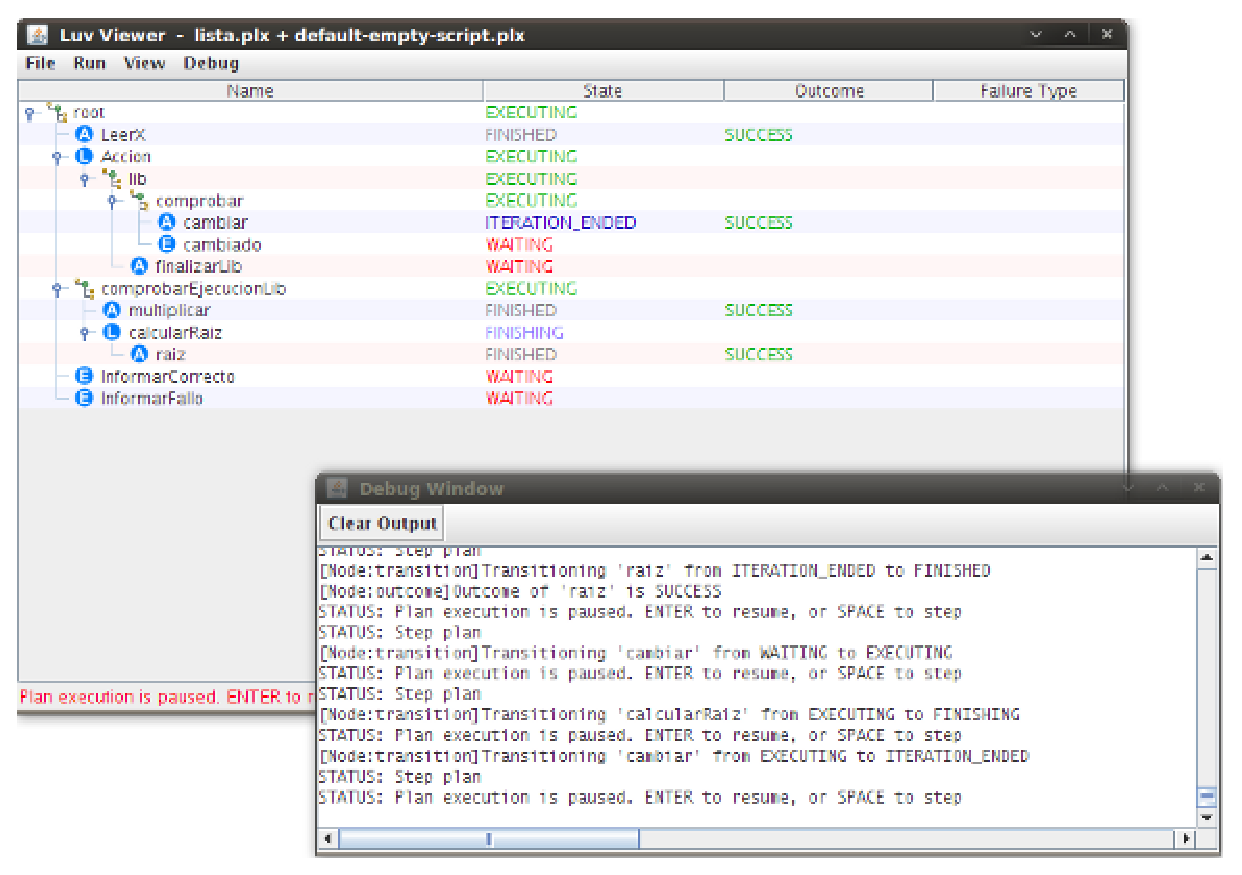
\includegraphics[width=10cm]{luv}
 \caption{Ventana principal y de debug de Luv}
 \label{fig:luv}
\end{center}
\end{figure}

A continuaci�n se describen las opciones que permite Luv:
\begin{itemize}
	\item Permite pausar la ejecuci�n del plan y reanudarla. Adem�s, permite la ejecuci�n paso a paso del plan o detener la ejecuci�n en los nodos deseados mediante puntos de ruptura. Los puntos de ruptura podr�n definirse en base al cambio de estado del nodo, al encontrarse el nodo en un estado en particular, por un estado de salida o por un estado de fallo. 
	\item Muestra los nodos en la estructura de �rbol del plan, pudiendo mostrar u ocultar las ramas seg�n nuestras necesidades. Tambi�n permite mostrar u ocultar nodos por nombre o por tipo de nodo y la b�squeda de nodos por nombre.
	\item Puede generar archivos de depuraci�n con los elementos deseados a trav�s de una interfaz gr�fica.
	\item Permite obtener toda la informaci�n relativa a un nodo. La informaci�n proporcionada vendr� dada en funci�n del tipo de nodo y de los datos de que disponga, informando as� de las variables declaradas y su valor (s�lo el valor inicial), las condiciones definidas, y los datos asociados al tipo de nodo (comando, asignaci�n, etc).
\end{itemize}


\section{Funcionamiento del \textit{Universal Executive}}

En esta secci�n vamos a describir el funcionamiento del UE para ejecutar los planes escritos en PLEXIL. Para ello se dar� una descripci�n de como transcurre el estado de todos los nodos (y, por tanto, del plan en s�) en el tiempo sin entrar en detalle de los algoritmos que llevan a cabo tareas de m�s bajo nivel, como por ejemplo la sincronizaci�n ante condiciones de carrera. Adem�s, una parte importante (aunque como ya se dijo, externa al UE) para la ejecuci�n es el arbitrador de recursos. El funcionamiento de �ste se ver� en la secci�n \ref{sec:uearec}.


\begin{comment}
El funcionamiento del flujo de ejecuci�n del UE se puede equiparar a una b�squeda primero en anchura en �rbol de estados. En este caso, al contrario que sucede en un problema de b�squeda convencional, no es necesario definir una funci�n sucesor para los nodos o expandirlos. Esto se debe a que el propio plan implementa la estructura de �rbol jer�rquico con el factor de ramificaci�n y profundidad descritos por el programador. Otra diferencia entre el problema de b�squeda y la ejecuci�n para la resoluci�n del plan de PLEXIL, es que en el problema de b�squeda la soluci�n es un camino que permita llegar desde el nodo ra�z a un nodo objetivo del �rbol. En este sentido, resolver un plan de PLEXIL es llevar a cabo la ejecuci�n de los nodos uno a uno, de tal forma que el plan finalizar� cuando el nodo ra�z halla finalizado su ejecuci�n. En la secci�n \ref{sec:tipos} vimos que para que un nodo lista finalizara su ejecuci�n, todos sus hijos deb�an finalizar su ejecuci�n (independientemente del estado de salida), y, dado que para tener un plan con m�s de un nodo el nodo ra�z debe ser un nodo lista, el plan finalizar� cuando se todos los nodos hijos de la ra�z hayan finalizado su ejecuci�n y, adem�s, se satisfaga la condici�n de finalizaci�n del nodo ra�z.

Dado que la ejecuci�n del plan generalmente estar� influenciada por los eventos que se den en el mundo exterior (que potencialmente ser�n as�ncronos y no deterministas), el camino que se de durante la ejecuci�n del plan ser� condicionado y carecer� de importancia. Lo que determinar� el estado del plan ser� el estado interno de todos los nodos, es decir, cuales est�n en ejecuci�n, listos para ser ejecutados, o en espera de un evento. Podr�a ser factible pensar que el UE se comporta como un algoritmo de b�squeda local. En un a b�squeda local deseamos encontrar una configuraci�n o estado objetivo independientemente del camino seguido para llegar a ella. En el caso de PLEXIL, la configuraci�n objetivo es aquella en la que, independientemente del estado de salida, el nodo ra�z haya finalizado su ejecuci�n. No obstante, esta definici�n carece de valor, ya que para la ejecuci�n no se aplican funciones que eval�en el coste para pasar de un estado a otro, ya que las transiciones se llevar�n a cabo fundamentalmente debido a eventos externos y, adem�s, no hay una configuraci�n m�s "valida" que otra, ya que el prop�sito del plan es ejecutar todos los nodos que sea posibles.

�UE ~ Agente basado en modelos? 
\end{comment}


La ejecuci�n del UE se lleva a cabo a trav�s de ciclos de ejecuci�n que especifican qu�, c�mo y cu�ndo variar� el estado de los nodos en un instante espec�fico del tiempo. Cabe destacar que la ejecuci�n del plan proceder� en pasos discretos y que los eventos (cambios en el mundo que afecten a condiciones, valores de retorno de funciones o comandos, etc) ser�n procesados en el orden en que llegan (FIFO o primero en entrar, primero en salir). Esto implica que ante la misma sucesi�n de eventos en el tiempo, el UE se comportar� de forma determinista. Adem�s de procesar el evento, se procesar�n tambi�n las consecuencias que �ste tenga en cascada sobre el resto del plan, lo que se conoce como sem�ntica \textit{run-to-completion}\cite{ref:semantica}. Dichos eventos ser�n los que conduzcan como tal el flujo de ejecuci�n del plan.

En el punto de partida, el plan se encuentra en un estado inactivo. Esto quiere decir que todos los nodos estar�n detenidos y no afectar�n al mundo externo. El primer nodo en pasar a ejecuci�n ser� la ra�z y, en el instante siguiente, todos sus hijos pasar�n al estado de espera antes de ser ejecutados. En dicho estado, el nodo podr� entrar en ejecuci�n cuando se verifique su condici�n de inicio (siendo por defecto verdadera), pasando a ejecutar las acciones definidas en su cuerpo. Una vez ejecutado, el nodo se marcar� como iteraci�n finalizada y, en base a la presencia o no de una condici�n de repetici�n, su estado final de ejecuci�n ser� en espera para nodos con condici�n de repetici�n, o finalizado para nodos sin dicha condici�n. Hay una excepci�n a esta regla, los nodos lista, que tras su ejecuci�n pasar�n a un estado finalizando que indica que el nodo ha cumplido su objetivo y esta en espera de que sus nodos hijo hayan finalizado. En caso de que un nodo lista tenga condici�n de repetici�n, la lista completa podr� volver a ejecutarse cuando �sta se cumpla, pero no al rev�s.

Hay tres causas que marcar�n la finalizaci�n de un nodo: que complete su ejecuci�n, la presencia de fallos o eventos externos. En el primer caso, la finalizaci�n de un nodo depender� del tipo de �ste. Por ejemplo los nodos de asignaci�n terminar�n cuando se halla establecido el nuevo valor en la variable. En el caso de los nodos lista, si el nodo ha cumplido su condici�n de finalizaci�n pero sus nodos hijos no han terminado su ejecuci�n, se realizar� una terminaci�n limpia de los hijos de la forma que sigue:
\begin{enumerate}
	\item S�lo los nodos activados o en ejecuci�n continuar�n con sus procesos de forma concurrente.
	\item Los hijos pendientes de verificar sus condiciones de inicio no ser�n ejecutados.
	\item El padre esperar� a que los hijos en ejecuci�n finalicen.
\end{enumerate}

En el caso de que un nodo finalice por un fallo (pre/postcondici�n o condici�n invariante que no sea satisfecha), el nodo abortar� su ejecuci�n de forma abrupta, incluyendo el caso de los nodos lista, que no finalizar�n de la forma antes descrita. 

Una vez finalizado un nodo, si �ste tiene condici�n de repetici�n, los datos internos del nodo se reinicializar�n y el nodo volver� al estado de espera. En relaci�n a esto, hay que indicar que las condiciones del nodo, una vez activadas, no podr�n ser desactivadas posteriormente salvo por un reseteo del nodo. Esto quiere decir que si en un instante dado, un nodo en espera verifica tras un evento que su condici�n de inicio es correcta, el nodo comenzar� la ejecuci�n, aunque en el instante siguiente dicha condici�n se torne falsa nuevamente.


\subsection{Ciclos de ejecuci�n}

Los ciclos fundamentales de ejecuci�n de un plan PLEXIL ser�n los \textit{macro steps} y los \textit{atomic steps}. Los \textit{macro steps} ser�n los pasos discretos que se ejecutar�n en el plan. Dichos pasos est�n compuestos por \textit{micro steps} o ejecuci�n en paralelo de una serie de \textit{atomic steps}. Los \textit{atomic steps} act�an sobre cada nodo individual.

Como puede verse, el nivel de ejecuci�n inferior (refiri�ndose por inferior a que esta m�s alejado del mundo exterior y m�s centrado en el estado interno del plan) es el \textit{atomic step}, mientras que el nivel superior ser� el nivel de ejecuci�n, el cual puede verse como una serie de relaciones entre los estados del mundo exterior y el estado interno del plan. La ejecuci�n de un plan por tanto, podr� analizarse en base a las acciones llevadas a cabo por cada nivel de ejecuci�n de forma incremental partiendo desde el nivel inferior. En los siguientes apartados se llevar� a cabo el an�lisis del funcionamiento de cada nivel y se finalizar� poniendo todos los niveles en com�n para ver como se comporta la ejecuci�n completa del UE en el ciclo de ejecuci�n.

\subsubsection{\textit{Atomic step}}

Un paso at�mico o \textit{atomic step} define una operaci�n interna o una transici�n del estado para un nodo en un instante de tiempo. El paso at�mico representa una variaci�n de un dato interno del nodo que s�lo afectar� directamente a �ste y nunca al estado del mundo exterior. Hay un total de 37 reglas que definen las posibles transiciones de un nodo; �stas podr�n verse de forma gr�fica en el ap�ndice \ref{ap:transiciones}. Dichas reglas no ser�n aplicables a todos los nodos, dado que en ciertos estados las posibles transiciones entre estados variar�n en base al tipo de nodo.


\subsubsection{\textit{Micro step}}

Un \textit{micro step} representa la ejecuci�n paralela de varios pasos at�micos. Los nodos se ejecutan en paralelo, de tal forma que en un �nico instante de tiempo puede haber uno o m�s nodos realizando pasos at�micos. En este nivel se llevan a cabo varias tareas: se modifican los valores de salida y estado de los nodos en ejecuci�n y se llevan a cabo tareas de sincronizaci�n. Aqu� se establecen las pol�ticas que permitir�n resolver condiciones de carrera en caso de, por ejemplo, que dos nodos intenten acceder a una misma variable para asignarle un valor. En este caso, se utilizar� una regla de precedencia para evitar accesos simult�neos a recursos compartidos.


\subsubsection{\textit{Quiescence cycle}}

El ciclo de reposo o \textit{quiescence cycle} indica que se han realizado todos los \textit{micro steps} posibles hasta que todos los nodos que pod�an ser ejecutados han alcanzado un estado estable (a la espera de un evento, finalizado, etc). Es decir, el plan est� en un estado estable a la espera de nuevos eventos que permitan continuar con la ejecuci�n de nodos que esperan por ellos o por la finalizaci�n de nodos bloqueados hasta la llegada de los mismos.


\subsubsection{\textit{Macro step}}

Hasta este momento la ejecuci�n del plan se lleva a cabo s�lo alterando el estado interno del plan. En los \textit{macro steps} es donde se lleva a cabo la comunicaci�n entre el plan y los eventos producidos por el mundo exterior. 

Los \textit{macro steps} se inician con la llegada de un nuevo evento externo al sistema. Todos los nodos que estuvier�n esperando por dicho evento, realizar�n transiciones a su siguiente estado en paralelo a trav�s de \textit{micro steps}. Estas transiciones pueden provocar cambios internos que permitan transicionar a m�s nodos, con lo cual se llevar�n a cabo m�s \textit{micro steps} hasta que se finalice la secuencia de cambios en cascada. Es en ese momento cuando se alcanza el ya mencionado \textit{quiescence cycle}. Es decir, el estado de reposo se alcanza al final de un \textit{macro step}, el cual no es m�s que una secuencia de \textit{micro steps} ocasionados por la recepci�n de un evento. Una vez se finaliza el paso, el sistema puede atender nuevos eventos. Como se mencion� al principio de la secci�n, los eventos son atendidos en orden de llegada (FIFO) y hasta que un evento no haya sido ``despachado'' no se comenzar� a atender al siguiente.

Una particularidad importante es que los datos del mundo exterior relacionados con el plan s�lo ser�n le�dos en la primera utilizaci�n de cada \textit{macro step}, as� como a la finalizaci�n de �ste. Dicho de otra manera, se asume que los cambios del mundo exterior s�lo ser�n visibles al comienzo y al final del paso, y que una vez le�dos permanecer�n inalterados. Una vez le�do un dato, una nueva lectura del mismo dato en el mismo \textit{macro step} dar� el mismo valor aunque �ste haya cambiado en el mundo real. Con ello se consigue una optimizaci�n en el acceso a los valores necesarios del mundo real. 

Tambi�n hay que indicar que la ejecuci�n de comandos (o actuaciones sobre el mundo exterior) no las lleva a cabo el propio plan ni el UE, sino que se subrogan a un sistema de bajo nivel encargado de ejecutar las ordenes indicadas por el plan. En este sentido, un nodo de comando solicitar� la ejecuci�n de un comando determinado y podr� continuar su ejecuci�n o esperar a que el mundo exterior genere un evento como respuesta a dicha acci�n. La sincronizaci�n entre el UE y el soporte de bajo nivel se llevar� a cabo a trav�s de interfaces que se ver�n en la secci�n \ref{sec:ueframew}.


\subsubsection{Nivel de ejecuci�n}

El nivel o ciclo de ejecuci�n puede describirse como la sucesi�n de \textit{macro steps} y la lista de eventos que se producen en el mundo a lo largo del tiempo. Esto representa como evoluciona tanto el plan como el mundo desde el inicio hasta la finalizaci�n del plan. En este punto tambi�n pueden verse los efectos producidos por la ejecuci�n de las acciones indicadas por el plan de PLEXIL y ejecutadas por el soporte de bajo nivel asociado. En la figura \ref{fig:ciclosue} puede verse un esquema con todos los niveles de ejecuci�n.

\begin{figure}[h]
\begin{center}
 \includegraphics[width=12cm]{Ciclos}
 \caption{Representaci�n de los ciclos de ejecuci�n del UE}
 \label{fig:ciclosue}
\end{center}
\end{figure}

Finalmente hay que hacer una valoraci�n acerca de como se trata la ejecuci�n de PLEXIL en el tiempo. PLEXIL no hace valoraciones acerca de cuanto dura la ejecuci�n de un paso, al contrario de lo que suelen hacer otros lenguajes. Generalmente se asume que un paso (en este caso ser�a un \textit{micro step}) toma cero unidades de tiempo, o, dicho de otra forma, el mundo cambia con una frecuencia muy inferior a la duraci�n de los pasos de ejecuci�n. En PLEXIL esto no es importante, y se asume que si un \textit{micro step} tarda un tiempo mayor que cero, quiere decir que el \textit{macro step} en curso durar� un tiempo mayor que cero. Durante dicho periodo, si el mundo exterior var�a, puede ocurrir que los datos que utilice el plan sean obsoletos (s�lo se leen los datos externos al inicio y fin del \textit{macro step}. Esto tambi�n sucede cuando un evento se procesa mucho despu�s de haber sido recibido. En estos casos, la lectura de los datos al final del \textit{macro step} provocar� que se actualice la informaci�n y se descarte aquella que fuera obsoleta.



\section{Arbitrador de recursos}\label{sec:uearec}

PLEXIL permite construir la lista de recursos necesarios para poder ejecutar un determinado comando. El arbitrador de recursos, integrado como una parte del UE, implementa la l�gica necesaria para poder operar con esa informaci�n y mantener actualizada la informaci�n del uso y disponibilidad de recursos. En base a esta informaci�n, el arbitrador de recursos podr� permitir o denegar los comandos que cumplan o no con las restricciones impuestas. La figura \ref{fig:resarbfes} muestra un esquema simple de los componentes e interacciones en los que est� involucrado el arbitrador de recursos.

\begin{figure}[h]
\begin{center}
 \includegraphics[width=12cm]{resarb}
 \caption{Esquema del arbitrador de recursos}
 \label{fig:resarbfes}
\end{center}
\end{figure}

El arbitrador de recursos ofrece las siguientes funcionalidades:
\begin{itemize}
	\item Implementa recursos renovables y no renovables, que pueden ser unarios o no unarios.
	\item El estado de los recursos y su consumo son gestionados por �l mismo. Esto asume que el consumo de cada comando es conocido con antelaci�n y fijo. S�lo gestionar� el uso de recursos de los comandos emitidos por el UE.
	\item No hace predicciones acerca del tiempo de duraci�n de los comandos o del instante en que el sistema real hace uso de los recursos. Esto quiere decir que el consumo de recursos se har� inmediatamente al permitir la ejecuci�n del comando, y, en caso de haber generaci�n de recursos, �sta tendr� lugar al finalizar el comando.
\end{itemize}

Tambi�n hay dos restricciones importantes en el arbitrador de recursos:
\begin{itemize}
	\item Todos los recursos utilizados en un mismo comando tienen la misma prioridad (es decir, realmente no se prioriza el uso de recursos, sino que se establece prioridad al comando). No obstante, cada recurso puede especificar su propia prioridad (XML y el compilador de PLEXIL lo permiten), pero el arbitrador de recursos s�lo tomar� la primera prioridad establecida y la utilizar� como prioridad de todos los recursos para el comando dado.
	\item El valor m�nimo del uso de recurso es ignorado (\texttt{LowerBound}).
\end{itemize}

Es importante destacar que el arbitrador de recursos s�lo se comunicar� con el UE, por tanto nunca podr� hacer consultas al sistema real para conocer el estado de los recursos o comprobar la disponibilidad de los mismos. Esto responde al esquema visto anteriormente: el grueso del sistema para la gesti�n de recursos es el arbitrador de recursos. Adem�s de �ste, los �nicos elementos afectados por el uso de recursos es el lenguaje (se considera que el tratamiento de los recursos por parte del lenguaje es una extensi�n de �ste) y el sistema externo, pues ser� el que finalmente haga uso de los recursos de que dispone. Por tanto, este sistema de control de recursos implica que en vez de enviar los comandos directamente al subsistema externo, el interfaz externo primero tiene que invocar el proceso de arbitraje y luego expedir s�lo los comandos aceptados al subsistema externo.


\subsection{Algoritmo del arbitrador}

Al arbitrador de recursos le llegar�n listas de comandos con sus respectivos usos de recursos desde el UE. El arbitrador entonces tendr� que gestionar los comandos para aceptar tantos comandos como sea posible comprobando que no se exceda el m�ximo permitido en el uso de los recursos asociados. Adem�s, deber� tener en cuenta si hay competencia entre comandos por el uso de los mismos recursos, en cuyo caso deber� tomar en cuenta la prioridad de cada comando para el uso de recursos y aceptar s�lo la ejecuci�n del comando con mayor prioridad.

El algoritmo de funcionamiento del arbitrador de recursos es el que se expone a continuaci�n:

\begin{enumerate}
	\item Para que un comando sea aceptado, todos los recursos que emplea deben estar disponibles en suficiente cantidad para llevarlo a cabo.
	\item El arbitrador optimiza tanto en prioridad de los recursos aceptados como en el n�mero total de estos.
	\item Un comando de menor prioridad s�lo ser� aceptado si una vez aceptados los de mayor prioridad hay suficientes recursos como para que �ste entre en ejecuci�n. Tambi�n puede darse el caso de que sea aceptado por haber denegado la ejecuci�n a los de mayor prioridad por no cumplir las restricciones de uso de recursos.
	\item Si dos recursos tienen la misma prioridad, estos ser�n ejecutados en el orden en el que han llegado al arbitrador al final del ciclo de espera. 
	\item Cuando un grupo de comandos ha sido aceptado, en el peor de los casos no se superar� el uso del m�ximo de los recursos permitidos a cada comando.
\end{enumerate}


\subsection{Archivo de configuraci�n de recursos}

Por defecto, el arbitrador de recursos obtiene la identidad de los recursos ejecutados en el plan directamente de los comandos, cuando un comando necesita un recurso en particular, el arbitrador lo a�ade a su base de datos, y, una vez completada la ejecuci�n del comando, dicho recuso ser� purgado de la base de datos del arbitrador. Adem�s, establece el valor m�ximo para recursos, tanto renovales como consumibles, en 1.0.

No obstante, el usuario tiene la opci�n de recolectar la informaci�n asociada al uso de recursos del sistema a implementar y plasmarla en un archivo de configuraci�n de recursos que podr� ser le�do por el arbitrador de recursos. La expresi�n m�nima de este archivo ser� una relaci�n de los recursos usados y los valores m�ximos de consumo y renovaci�n de estos. Adem�s podr� a�adir informaci�n acerca de las dependencias entre recursos. Como se mencion� anteriormente, se pueden crear jerarqu�as de recursos que deber�n ser indicadas en este fichero, representadas en forma de gr�fico dirigido y ponderado ac�clico. En la figura \ref{fig:graforec} se muestra un ejemplo de la estructura de una jerarqu�a de recursos y en la figura \ref{fig:filerec} el formato correspondiente para el archivo de configuraci�n. Los pesos representan el valor absoluto del consumo del recurso indicado. En caso de no indicar peso, implica que requiere el uso del recurso en su totalidad.

\begin{figure}[h]
\begin{center}
 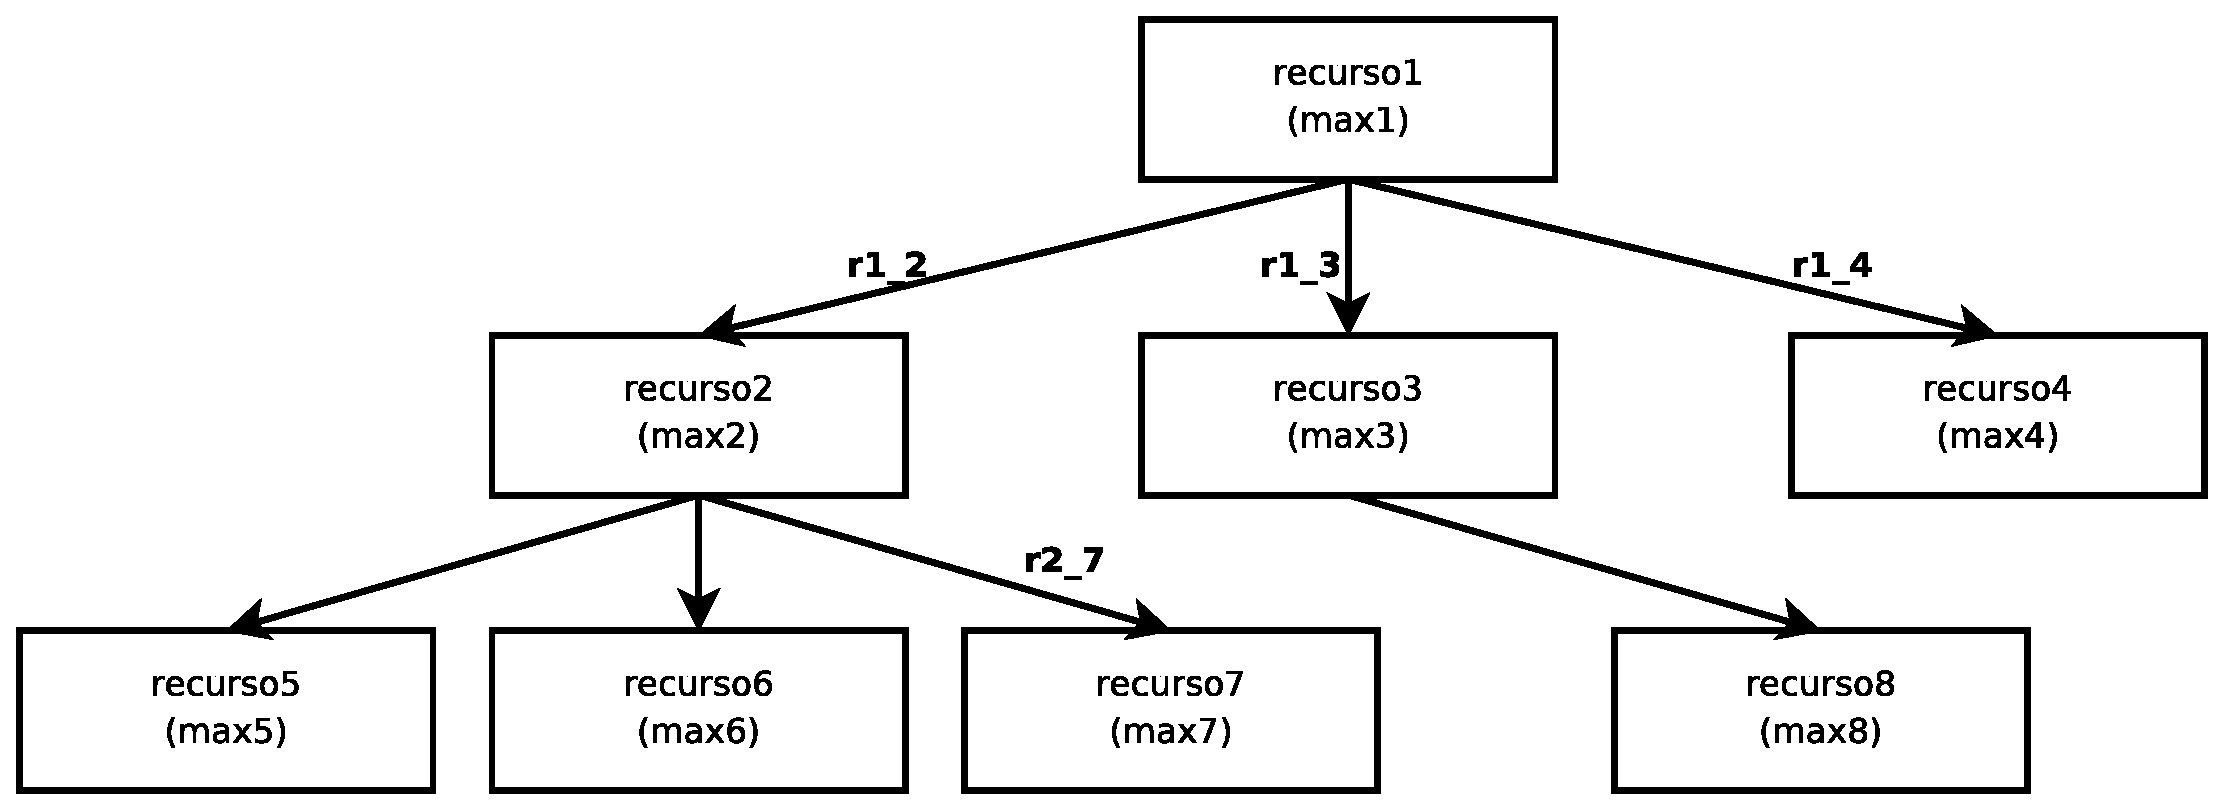
\includegraphics[width=12cm]{graforec}
 \caption{Grafo de jerarqu�a de recursos}
 \label{fig:graforec}
\end{center}
\end{figure}

\begin{figure}[!h]
\begin{center}
\begin{minipage}{12cm}
\lstset{language=c++, breaklines=true, tabsize=3}
\lstset{commentstyle=\textit}
\lstset{stringstyle=\ttfamily, basicstyle=\footnotesize}
\begin{lstlisting}[frame=trbl]{}
recurso1 max1 r1_2 recurso2 r1_3 recurso3 r1_4 recurso4
recurso2 max2 1.0  recurso5 1.0  recurso6 r2_7 recurso7
recurso3 max3 1.0  recurso8
recurso4 max4
recurso5 max5
recurso6 max6
recurso7 max7
recurso8 max8
\end{lstlisting}
\end{minipage}
\caption{Archivo de configuraci�n para el grafo de la figura \ref{fig:graforec}}
\label{fig:filerec}
\end{center}
\end{figure}

\section{\textit{Universal Executive Framework}}\label{sec:ueframew}

En esta secci�n se mostrar� una guia para poder crear una aplicaci�n que emplee el \textit{Universal Executive} como sistema de ejecuci�n para un plan modelado en PLEXIL. Se ver� de forma b�sica los elementos necesarios para instanciar el UE y el prototipo b�sico de una librer�a (que utilice s�lo comandos, no se ver�n \textit{lookups} o la implementaci�n de telemetr�a) conforme a la especificaci�n creada para dar soluci�n a una arquitectura t�pica de tres capas (3T) para la locomoci�n aut�noma de un robot hex�podo \cite{ref:Ptinto10}.

Para poder montar una aplicaci�n que haga uso del lenguaje PLEXIL ser�n necesarios dos elementos: 
\begin{itemize}
 \item \textbf{UE \textit{framework}}: ser� una instancia del \textit{universal executive framework} encargada de inicializar los elementos del ejecutor, fundamentalmente los interfaces (a partir del archivo de configuraci�n de interfaces que se ver� en la secci�n \ref{sec:configinf}) y los planes y librer�as escritas en PLEXIL (el plan a ejecutar). No ser� necesaria la modificaci�n del \textit{framework} para aplicaciones sencillas; los elementos necesarios para su instanciaci�n se ver�n en la secci�n \ref{sec:uecod}.
 \item \textbf{Una o m�s librer�as din�micas}: en funci�n de las directrices impuestas por el archivo de configuraci�n de interfaces se deber�n tener una o m�s librer�as din�micas que contengan la implementaci�n de los comandos y \textit{lookups} empleados en el plan PLEXIL. La forma de crear estas librer�as se vera en la secci�n \ref{sec:libso} y requieren la especificaci�n de una serie de funciones virtuales.
\end{itemize}

El funcionamiento de una aplicaci�n que emplee el lenguaje PLEXIL y el ejecutor UE a la hora de realizar un comando es el que se muestra en la figura \ref{fig:comando}. Cuando un plan PLEXIL invoca un comando, el \textit{framework} del UE (esto es, el ejecutor) solicita a la interfaz que lleve a cabo el comando. La interfaz del ejecutor posee un archivo de configuraci�n definido por el usuario (archivo de configuraci�n de interfaces) que indica que comandos se pueden llevar a cabo y que librer�a din�mica implementa dicho comando. Una vez localizada la librer�a para el comando solicitado se asignar� un manejador de comando desde el ejecutor y se solicitar� a la librer�a que lleve a cabo el c�digo de la funci�n asociada a dicho comando. Dentro de dicho c�digo se podr� actualizar tanto el estado del manejador de comando, como el valor de retorno del comando si lo tuviera. La librer�a para poder operar de cara al ejecutor deber� poseer una interfaz espec�fica que permita al ejecutor la solicitud de comandos de forma gen�rica.

\begin{figure}[h]
\begin{center}
 \includegraphics[width=14cm]{ComandoUE}
 \caption{Flujo de ejecuci�n de un comando}
 \label{fig:comando}
\end{center}
\end{figure}


\subsection{Archivo de configuraci�n de interfaces}\label{sec:configinf}

El archivo de configuraci�n de interfaces ser� un archivo con codificaci�n XML que indicar� las librer�as empleadas por el plan PLEXIL, comandos y \textit{lookups} que lleva a cabo cada una de ellas. La etiqueta de mayor nivel del archivo ser� \texttt{Interfaces}. Por cada librer�a din�mica a emplear se deber� definir un adaptador de interfaz mediante la etiqueta \texttt{Adapter} y el atributo \texttt{AdapterType= "\textit{nombre\_libreria}"}, donde \textit{nombre\_libreria} es el nombre de la librer�a din�mica a emplear (sin necesidad de extensi�n ni el prefijo \texttt{lib} est�ndar).

Tras esto se podr�n declarar para cada adaptador la lista de comandos o \textit{lookups} de los cuales se encarga cada librer�a. Ambos casos ser�n una lista de los nombres de los comandos (sin lista de par�metros ni tipo de retorno si lo tuvieran) separados por comas. La etiqueta que define el listado de comandos es \texttt{CommandNames} y para los \textit{lookups} ser� \texttt{LookupNames}. En el caso de que se quiera declarar una librer�a a la que asociar todos los comandos que no se han asociado explicitamente con otra librer�a, se deber� poner la etiqueta \texttt{DefaultAdapter} tras el identificador del adaptador.

En la figura \ref{fig:ejinfich} se muestra un archivo de interfaces de ejemplo. Adem�s de las librer�as que creemos para nuestra propia aplicaci�n, la distribuci�n de PLEXIL incorpora algunas librer�as con �tiles como gesti�n de \textit{sockets}, utilidades variadas, gesti�n del tiempo del sistema operativo nativo (\texttt{OSNativeTime}) y el adaptador \texttt{Dummy} que retorna siempre COMMAND\_SUCCESS.

\begin{figure}[!h]
\begin{center}
\begin{minipage}{12cm}
\lstset{language=xml, breaklines=true, tabsize=3}
\lstset{commentstyle=\textit}
\lstset{stringstyle=\ttfamily, basicstyle=\footnotesize}
\begin{lstlisting}[frame=trbl]{}
<Interfaces>
	<Adapter AdapterType="OSNativeTime">
		<LookupNames>
		time
		</LookupNames>
 	</Adapter>
 	<Adapter AdapterType="Dummy">
		<DefaultAdapter/>
	</Adapter>
		<Adapter AdapterType="PDDLue">
		<CommandNames>
		crear_planificador, planificar, sig_accion,
		insertar_predicado, modificar_predicado,
		objeto_predicado, objeto_accion, valor_funcion,
		</CommandNames>
		<LookupNames>
		duracion
		</LookupNames>
	</Adapter>
</Interfaces>
\end{lstlisting}
\end{minipage}
\caption{Ejemplo de archivo de configuraci�n de interfaces}
\label{fig:ejinfich}
\end{center}
\end{figure}


\subsection{Implementaci�n del ejecutor}

En esta secci�n se mostrar� de forma breve mediante un ejemplo los elementos necesarios para instanciar el ejecutor UE y la creaci�n de una librer�a din�mica que sea capaz de interactuar con �l. El esquema b�sico de la aplicaci�n es el que se muestra en la figura \ref{fig:clases}, en la cual se puede distinguir en la parte superior el programa principal que hace uso de una clase que instancia el ejecutor, as� como una clase C++ que ha heredado la clase \texttt{InterfaceAdapter} y emplea las funciones de una librer�a para dar servicio al ejecutor. Adem�s se pueden ver las dependencias directas del c�digo de la distribuci�n de PLEXIL que tiene cada elemento.

\begin{figure}[h]
\begin{center}
 \includegraphics[width=9cm]{clases}
 \caption{Esquema de la arquitectura empleada}
 \label{fig:clases}
\end{center}
\end{figure}

Lo mostrado en las siguientes secciones ser� el desarrollo empleando la versi�n 0.90 de la distribuci�n de PLEXIL. En versiones posteriores pueden darse cambios. La distribuci�n de archivos dentro de una carpeta ra�z (sea \texttt{src}) empleada es la siguiente:
\begin{itemize}
 \item \texttt{main}: codigo fuente de la funci�n principal del programa.
 \item Carpeta \textit{comandos}: aqu� se encuentra el c�digo fuente para crear la librer�a est�tica \texttt{comandos}.
 \item Carpeta \textit{PLEXIL}: dentro de esta carpeta se encuentran los archivos \texttt{Makefile} para crear el ejecutor y la librer�a din�mica. Ademas se encuentra el c�digo asociado a los mismos (una clase por cada uno: \texttt{run\_UE} y \texttt{comandosInterfaceAdapter} respectivamente) y dos subcarpetas:
 \begin{itemize}
  \item Carpeta \textit{tinyxml}: esta carpeta proviene de la distribuci�n de PLEXIL y tiene los componentes necesarios del parseador XML.
  \item Carpeta \textit{src}: aqu� se encuentran los componentes de PLEXIL. Estar� compuesta por las carpetas \textit{app-framework}, \textit{exec} y \textit{utils} que se pueden encontrar en \texttt{\$PLEXIL\_HOME/src}.
 \end{itemize}
\end{itemize}


\subsubsection{Implementaci�n del \textit{framework} del UE}\label{sec:uecod}

Para poder compilar los elementos necesarios del \textit{framework} en la carpeta \textit{app-framework} se encuentra un archivo \texttt{Makefile} que podemos adaptar a nuestras necesidades con el fin de compilar el sistema de ejecuci�n de nuestra aplicaci�n.

En este ejemplo en concreto tendremos una clase que instanciar� los elementos del ejecutor \texttt{run\_UE} y una clase \texttt{main} que se encargar� de crear el resto del contenido de nuestra aplicaci�n. Adem�s se har� uso de una librer�a din�mica (\texttt{comandos}), que es en origen el c�digo de una librer�a est�tica. El \texttt{Makefile} empleado es el que se muestra en la figura \ref{fig:makeexec}\footnote{Se ha omitido la licencia contenida en el \texttt{Makefile} original.}.

\begin{figure}[!h]
\begin{center}
\begin{minipage}{12cm}
\lstset{language=bash, breaklines=true, tabsize=3}
\lstset{commentstyle=\textit}
\lstset{stringstyle=\ttfamily, basicstyle=\footnotesize}
\begin{lstlisting}[frame=trbl]{}
include makeinclude/standard-defs.make
EXECUTABLE	:= a.out

# External dependencies
INC_DIRS	+= tinyxml src/utils src/exec src/app-framework ../comandos ../../include
LIB_PATH	+= ../../lib
LIBS		+= tinyxml PlexilUtils PlexilExec PlexilAppFramework Comandos dl
SRC		:= ../main.cpp run_UE.cpp
INC		:= 

include makeinclude/standard-targets.make
ifneq (\$(MAKECMDGOALS),clean)
-include Makedepend
endif
\end{lstlisting}
\end{minipage}
\caption{Ejemplo de \texttt{Makefile} para el ejecutor}
\label{fig:makeexec}
\end{center}
\end{figure}

El archivo \texttt{run\_UE} es b�sicamente una copia del archivo \texttt{\$PLEXIL\_HOME/src/app- framework/test/testMain.cc} el cual permite instanciar mediante el par�metros (para definir el plan PLEXIL, librer�as PLEXIL, archivo de configuraci�n de interfaces y archivo de depuraci�n) el ejecutor y ejecutar el plan PLEXIL indicado.

\subsubsection{Implementaci�n de una librer�a din�mica para el UE}\label{sec:libso}

Para utilizar una librer�a en un plan PLEXIL se deber� implementar la clase C++ \texttt{InterfaceAdapter} de forma que de soporte a nuestras necesidades. Dicha clase posee una serie de funciones virtuales para permitir codificar el funcionamiento de los comandos y \textit{lookups}. El funcionamiento de ambos es similar, de tal forma que la ejecuci�n de un comando en un plan PLEXIL implica una llamada a la funci�n \texttt{executeCommand} con una serie de par�metros que permiten conocer el nombre del comando, los par�metros utilizados al invocar el comando y el manejador asociado a �ste. Con ello se podr�n realizar las llamadas pertinentes a las funciones implementadas en el sistema externo, de tal forma que el resultado obtenido por dichas funciones podr� ser devuelto al ejecutor a trav�s del manejador de comando asociado, mediante la funci�n \texttt{handleValueChange}. Adem�s con la misma funci�n se puede asociar al manejador el estado de ejecuci�n del comando en cualquier momento durante la ejecuci�n del mismo. Dicho estado acepta los valores vistos en la secci�n \ref{sec:mcom}.

Al igual que en el caso anterior, dispondremos de un \texttt{Makefile} gen�rico que podremos adaptar para crear nuestra propia librer�a. El archivo empleado para este ejemplo es el que se muestra en la figura \ref{fig:makelib}. Con ello obtendremos la librer�a \texttt{libComandos.so} que podremos emplear para dar servicios a los planes PLEXIL que utilicen los comandos implementados.

\begin{figure}[!h]
\begin{center}
\begin{minipage}{12cm}
\lstset{language=bash, breaklines=true, tabsize=3}
\lstset{commentstyle=\textit}
\lstset{stringstyle=\ttfamily, basicstyle=\footnotesize}
\begin{lstlisting}[frame=trbl]{}
include makeinclude/standard-defs.make
OSTYPE   ?= $(shell uname -s)
MACHTYPE ?= $(shell uname -p)
OS_ARCH = $(OSTYPE)-$(MACHTYPE)

LIBRARY := Comandos
LIBRARY_SRC := comandosInterfaceAdapter.cpp 
LIBRARY_OBJ := $(LIBRARY_SRC:.cpp=.o)
INC_DIRS += tinyxml src/utils src/exec src/app-framework ../comandos ../../include
LIBS += tinyxml Comandos
LIB_TARGET = lib$(LIB_NAME)$(LIB_EXT)

include makeinclude/standard-targets.make
# these must follow the above 'include'
$(SHLIB): depend $(LIBRARY_OBJ)
	$(LD) $(SHARED_FLAGS) $(LIB_PATH_FLAGS) $(LIB_FLAGS) -o $@ $(LIBRARY_OBJ)
$(ARCHIVE): $(LIBRARY_OBJ) depend
	$(AR) -o $@ $(LIBRARY_OBJ)
-include Makedepend
\end{lstlisting}
\end{minipage}
\caption{Ejemplo de \texttt{Makefile} para una librer�a din�mica}
\label{fig:makelib}
\end{center}
\end{figure}

El archivo \texttt{comandosInterfaceAdapter} ser� una clase C++ que hereda de la clase \texttt{PLEXIL::InterfaceAdapter}. Con ello dispondremos de una serie de funciones virtuales que deberemos implementar para dar soporte a la interfaz con el ejecutor. En este ejemplo s�lo se ver� el funcionamiento de los comandos. Se ver� c�mo se reciben los comandos, el parseo de par�metros, modificaci�n del estado del manejador de comando y el retorno de un valor como resultado de la ejecuci�n del comando.

Antes de crear cualquier otro elemento de c�digo habr� que registrar el adaptador como se muestra en la figura \ref{fig:regadapter}.

\begin{figure}[!h]
\begin{center}
\begin{minipage}{12cm}
\lstset{language=c++, breaklines=true, tabsize=3}
\lstset{commentstyle=\textit}
\lstset{stringstyle=\ttfamily, basicstyle=\footnotesize}
\begin{lstlisting}[frame=trbl]{}
extern "C" {
	void initcomandos() {
		REGISTER_ADAPTER(comandosInterfaceAdapter,"Comandos");
	}
}
\end{lstlisting}
\end{minipage}
\caption{Registro del adaptador de una librer�a}
\label{fig:regadapter}
\end{center}
\end{figure}

Una vez hecho esto podremos pasar a implementar las funciones necesarias para que la librer�a cumpla su cometido. Aqu� s�lo se ver�n los elementos b�sicos, pero se puede definir el comportamiento deseado en funci�n de las necesidades de la librer�a y la aplicaci�n para, por ejemplo, la inicializaci�n de la librer�a, finalizaci�n, reinicio de la misma, etc. Si deseamos que la librer�a disponga de datos iniciales o si tiene que crear una estructura de datos en su inicializaci�n, se podr� incluir el c�digo necesario en la funci�n \texttt{initialize()}. Adem�s en dicha funci�n habr� que iniciar un atributo heredado que permitir� conectar la librer�a con la interfaz del ejecutor. Para ello habr� que emplear la instrucci�n \texttt{m\_execInterface.defaultRegisterAdapter(getId());}. El resto de funciones (\texttt{start()}, \texttt{stop()} o \texttt{reset()} por ejemplo) se pueden dejar con un simple \texttt{return true;} si no se requiere que tengan un comportamiento espec�fico.

Las funciones que dan soporte a la interfaz del ejecutor son \texttt{lookupNow()}, \texttt{lookup OnChange()} y \texttt{executeCommand()}. Las primeras se encargan de las solicitudes de \textit{lookups} y la �ltima, en la que entraremos en m�s detalle, de los comandos.

A la hora de recibir un comando, el punto de entrada a nuestro c�digo ser� la funci�n \texttt{executeCommand} que recibir� una cadena de texto (en formato \texttt{PLEXIL::LabelStr}, consulte la documentaci�n de PLEXIL para familiarizarse con dicha clase) que contendr� el nombre del comando a ejecutar, as� como la lista de argumentos con la que ha sido invocado, la variable destino para el valor de retorno del comando y el manejador del comando que permitir� notificar al ejecutor en que estado de ejecuci�n se encuentra nuestro comando en cada momento.

Una vez tengamos la identificaci�n del comando solicitado deberemos proceder a ejecutar el c�digo pertinente. Una de las primeras cuestiones ser� notificar al ejecutor que el comando ha sido recibido, para ello se emplear� la funci�n \texttt{handleValueChange()}, siendo los par�metros el manejador de comando y la variable que determina el nuevo estado del manejador (pueden verse los estados posibles en la secci�n \ref{sec:mcom}). Una vez modificado el valor del manejador se deber� notificar el cambio al ejecutor para que �ste modifique su estado interno. Ello se hace con la funci�n \texttt{notifyOfExternalEvent()}. Es importante mencionar que estas funciones operan directamente sobre el objeto \texttt{m\_execInterface}. En cualquier momento se podr� modificar el estado del manejador del comando, as� como notificar el valor de retorno del comando. Esto tambi�n se har� con la funci�n \texttt{handleValueChange()} pero se emplear� como par�metro la variable destino indicada como par�metro en la funci�n de entrada. Hay que tener en cuenta que todos los valores notificados al ejecutor deber�n de ser de tipo \textit{double}, de tal forma que las cadenas de caracteres deber�n ser convertidas a objetos \texttt{LabelStr} que est�n definidos por un identificador de tipo \textit{double}, o se deber�n emplear los objetos de la clase \texttt{BooleanVariable} para definir los tipos booleanos. Una vez actualizado el valor de la variable no ser� necesario notificar al ejecutor de dicho cambio.

Finalmente, una vez ejecutado el c�digo de nuestra funci�n, antes de que finalice la funci�n \texttt{executeCommand()} se deber� modificar el resultado del comando (COMMAND\_SUCCESS o COMMAND\_FAILED) y notificar el cambio en el manejador al ejecutor como se ha visto anteriormente. En la figura \ref{fig:codlib} se puede ver un ejemplo para una funci�n \texttt{executeCommand()} que da servicio a dos comandos.

\begin{figure}[!h]
\begin{center}
\begin{minipage}{12cm}
\lstset{language=c++, breaklines=true, tabsize=3}
\lstset{commentstyle=\textit}
\lstset{stringstyle=\ttfamily, basicstyle=\footnotesize}
\begin{lstlisting}[frame=trbl]{}
void PDDLInterfaceAdapter::executeCommand(const PLEXIL::LabelStr& name, const std::list<double>& args, PLEXIL::ExpressionId dest, PLEXIL::ExpressionId ack)
{
    bool success = true;
    std::string nStr = name.toString();
    std::list<double>::const_iterator largs = args.begin();
    int nplanner = static_cast<int> (*largs);
    m_execInterface.handleValueChange(ack, PLEXIL::CommandHandleVariable::COMMAND_RCVD_BY_SYSTEM());
    m_execInterface.notifyOfExternalEvent();
    if(nStr == "comando1")
    {
        PLEXIL::LabelStr arg1(*largs);
        printf("Argumento: \%s",(char*)arg1.c_str());
        ultimaacc.push_back(new stpredicado);
        unsigned int num = 1;
        m_execInterface.handleValueChange(dest,num);
    }
    else if(nStr == "comando2")
    {
        bool arg2 = static_cast<bool> (*(++largs));
        if(!arg2)
	        success=false;
        m_execInterface.handleValueChange(dest,success?PLEXIL::BooleanVariable::TRUE():PLEXIL::BooleanVariable::FALSE());
    }
    
    if(success)
        m_execInterface.handleValueChange(ack, PLEXIL::CommandHandleVariable::COMMAND_SUCCESS());
    else
        m_execInterface.handleValueChange(ack, PLEXIL::CommandHandleVariable::COMMAND_FAILED());
    m_execInterface.notifyOfExternalEvent();
}
\end{lstlisting}
\end{minipage}
\caption{Ejemplo de funci�n \texttt{executeCommand()} para dos comandos}
\label{fig:codlib}
\end{center}
\end{figure}

\subsubsection{Implementaci�n de una librer�a din�mica para el UE a partir de SampleAdapter}\label{sec:salibso}

Para la implementaci�n de una librer�a din�mica para el UE, se propone la edici�n y adaptaci�n por parte del programador de un entorno desarrollado por la \textit{Universities Space Research Association} (USRA), cuyo c�digo se puede encontrar dentro del repositorio de PLEXIL. Dentro de los archivos que se necesitan para la implementaci�n, encontramos dos archivos fuente (y sus correspondientes \textit{headers}) \texttt{types.cc} y \texttt{subscriber.cc} que ser�n comunes a todas las interfaces a desarrollar, as� como otros dos archivos fuente espec�ficos, \texttt{SampleAdapter.cc} y \texttt{sample\_system.cc}. 

Internamente, PLEXIL trata todos los tipos de datos como \texttt{double}, pese a su definici�n en \texttt{Int}, \texttt{Real}, \texttt{String}, \texttt{Bool} y \texttt{Array}. El primer archivo fuente, \texttt{types.cc} y \texttt{types.hh} crea unas funciones muy �tiles para poder transformar todos los tipos de datos que se utilicen en la librer�a, a los datos utilizados en PLEXIL. Destacando un tipo de dato \texttt{Any} que se utilizar� especialmente para la gesti�n de los estados y \textit{lookups} de la librer�a. Esta abstracci�n que aporta este archivo, facilita el trabajo para evitar el empleo de operadores \textit{cast}. Estas funciones son del tipo \texttt{encodeTYPE} y \texttt{decodeTYPE}, siendo \texttt{TYPE} el tipo de dato que admite PLEXIL.

Por otra parte, \texttt{subscriber.cc} y \texttt{subscriber.hh} implementan funciones para la actualizaci�n de los valores de los estados utilizados en la librer�a a implementar. Por su forma de implementaci�n mediante sobrecarga del m�todo \texttt{publish}, se hace m�s sencillo la modificaci�n de un estado, sin atender al tipo de dato de estado, par�metros necesarios, etc. 

El primero de los archivos a modificar es \texttt{SampleAdapter.cc}. Se propone no a�adir m�todos a la clase directamente en este archivo fuente, dado que ese es el objetivo de \texttt{sample\_system}. Por una parte, debemos implementar las operaciones que deseemos en el \texttt{executeCommand}, que ser�n ejecutadas seg�n el plan de PLEXIL creado, as� como el control de los \textit{lookups} en el m�todo \texttt{lookupNow} que se explica a continuaci�n.

Cuando el UE encuentra un nodo del tipo \textit{Command node}, llama al m�todo \texttt{executeCommand} indic�ndole el nombre del comando, mediante \texttt{PLEXIL::LabelStr}, una lista de argumentos del tipo \texttt{Any} visto anteriormente, y los argumentos \texttt{dest} y \texttt{ack} del tipo \texttt{PLEXIL::ExpressionId} utilizados por el UE para el manejador de comandos, que indicara si ha sido ejecutado correctamente, y la valor de retorno de la funci�n. El funcionamiento de este m�todo es simple, compara el nombre del comando a ejecutar (\texttt{PLEXIL::LabelStr command\_name}) con los valores (\textit{string} o \texttt{PLEXIL::LabelStr}) de aquellos comandos a implementar, y llama a la funci�n correspondiente. En caso de no coincidir con ning�n comando, se mostrar� un error. 

Por �ltimo, en caso de devolver un valor, se pasar� mediante el manejador. Los argumentos del comando, son pasados mediante una lista de objetos tipo \texttt{Any}, que ser�n convertidos a tipos de datos de PLEXIL, mediante el uso de las funciones \texttt{encodeTYPE} y \texttt{decodeTYPE} vistas anteriormente.

\begin{figure}[!h]
\begin{center}
\begin{minipage}{12cm}
\lstset{language=c++, breaklines=true, tabsize=3}
\lstset{commentstyle=\textit}
\lstset{stringstyle=\ttfamily, basicstyle=\footnotesize}
\begin{lstlisting}[frame=trbl]{}
void EjemploAdapter::executeCommand (const LabelStr& command_name, const list<Any>& args, PLEXIL::ExpressionId dest, PLEXIL::ExpressionId ack) 
{
	// name contiene el nombre del comando ejecutado por el UE
  string name = command_name.toString();
  debugMsg("EjemploAdapter", "executeCommand recibido " << name);  

	// Variable para el resultado, en caso de necesitar return
  Any resultado = Unknown;
  
	// Lista de argumentos del comando
  vector<Any> argv(10);
  copy (args.begin(), args.end(), argv.begin());

  if (name == "Funcion1")
  {
  	// Este comando no devuelve valor, pasa un �nico argumento (Real) a la funci�n
	setValorX (decodeReal (*args.begin()));
  } else if (name == "Funcion2")
  {
  	// Este comando no devuelve valor, pasa dos argumentos
	avanzaRover (decodeReal(argv[0]), decodeReal(argv[1]), decodeInt (argv[2]));
  } else if (name == "CalculaAltura")
  {
  	// Este comando devuelve el valor retornado por la funci�n calculaAltura
	resultado = calculaAltura (decodeInt (*args.begin()));
  } else cerr << error << "Comando no valido: " << name << endl;

  // Manda un renorno al manejador de comandos del UE
  m_execInterface.handleValueChange
    (ack, PLEXIL::CommandHandleVariable::COMMAND_SENT_TO_SYSTEM());

  // Devuelve el resultado del comando, si procede
  if (dest != PLEXIL::ExpressionId::noId()) {
    m_execInterface.handleValueChange (dest, resultado);
  }

  m_execInterface.notifyOfExternalEvent();
}
\end{lstlisting}
\end{minipage}
\caption{Ejemplo de funci�n \texttt{executeCommand()} basado en SampleAdapter.cc}
\label{fig:excomlib}
\end{center}
\end{figure}

Como se puede apreciar en la figura \ref{fig:excomlib}, el uso tan s�lo de llamadas a las funciones de ejemplo \texttt{setValorX}, \texttt{avanzaRover} y \texttt{calculaAltura} simplifica la sintaxis del c�digo. Estas funciones, son funciones externas al presente c�digo, y a modo de ejemplo, se implementar�n en el archivo \texttt{sample\_system.cc}.

Durante el desarrollo de este documento, se ha explicado el significado y el uso de los \textit{lookups} en el c�digo, que atienden a modificaciones externas del estado del sistema. En caso de alteraci�n del valor de un estado, el ejecutor llama al m�todo \texttt{lookupNow} a continuaci�n (figura \ref{fig:lookuplib}). Este m�todo, seg�n se desarrolla en el ejemplo, toma el nombre del estado modificado, as� como de los argumentos de este para su actualizaci�n de informaci�n. Dependiendo de la aplicaci�n que se desee desarrollar, no es necesario la modificaci�n del c�digo perteneciente a \texttt{lookupNow}, s� en cambio la funci�n \texttt{fetch}.

La funci�n \texttt{fetch}, de tipo \texttt{Any} hace una selecci�n del estado que se desea modificar, entre los que se quieran tener disponibles, de una forma muy similar a lo visto en \texttt{executeCommand},  y se pasan los argumentos por referencia, mediante las funciones (\texttt{getX} y \texttt{setX}) creadas en el archivo \texttt{sample\_system.cc}.

\begin{figure}[!h]
\begin{center}
\begin{minipage}{12cm}
\lstset{language=c++, breaklines=true, tabsize=3}
\lstset{commentstyle=\textit}
\lstset{stringstyle=\ttfamily, basicstyle=\footnotesize}
\begin{lstlisting}[frame=trbl]{}
double EjemploAdapter::lookupNow (const State& state)
{
  // Nombre del estado que se vaya a modificar, y sus argumentos
  LabelStr name (state.first);
  const vector<Any>& args = state.second;
  return fetch(name.toString(), args);
}
\end{lstlisting}
\end{minipage}
\caption{Ejemplo de funci�n \texttt{lookupNow()} basado en SampleAdapter.cc}
\label{fig:lookuplib}
\end{center}
\end{figure}


\begin{figure}[!h]
\begin{center}
\begin{minipage}{12cm}
\lstset{language=c++, breaklines=true, tabsize=3}
\lstset{commentstyle=\textit}
\lstset{stringstyle=\ttfamily, basicstyle=\footnotesize}
\begin{lstlisting}[frame=trbl]{}
static Any fetch (const string& state_name, 
						const vector<Any>& args)
{
  debugMsg("EjemploAdapter:fetch",
           "Llamada a Fetch de  " << state_name << ", argumentos ( " << args.size() << " ) " );

  Any resultado;

  if (state_name == "Estado1")
  { 
  	resultado = encodeReal (getEstado1(decodeReal(args[0])));
  } ...
   else {
    cerr << error << " estado no valido: " << state_name << endl;
    resultado = Unknown;
  }
  debugMsg("EjemploAdapter:fetch",
           "Valor retornado por Fetch: " << 
           PLEXIL::Expression::valueToString (resultado));
  return resultado;
}
\end{lstlisting}
\end{minipage}
\caption{Funci�n \texttt{fetch()} basado en SampleAdapter.cc}
\label{fig:fetchlib}
\end{center}
\end{figure}

Con todo lo visto anteriormente, el archivo \texttt{sample\_system.cc} deber� contener los prototipos y desarrollos de las funciones que son accedidas desde el \texttt{executeCommand}, as� como la definici�n de los estados y sus funciones \texttt{setX} y \texttt{getX}. Este archivo es, principalmente, el que va a llevar toda la carga de funcionalidad para procesar los datos desde los \texttt{Command nodes} de PLEXIL. Por conveniencia, se propone el uso de diferentes archivos con estas funcionalidades, para las distintas librer�as que se deseen crear, a fin de agilizar y depurar con facilidad, pero no hay ninguna regla que lo impida. A continuaci�n, se muestra un ejemplo con las diferentes partes que componen este c�digo de ejemplo. En la figura \ref{fig:estSS} se definen los estados del sistema como variables de tipo \texttt{static}, que pueden o no ser inicializadas. En la figura \ref{fig:getsetSS}, mediante la funci�n \texttt{defAccessors} se generan autom�ticamente las funciones \texttt{getX} y \texttt{setX}. Por �ltimo, la figura \ref{fig:comSS} contiene un pseudoejemplo de un prototipo de funci�n que es llamada desde \texttt{executeCommand}, donde se deber� implementar toda la funcionalidad que se necesite para la ejecuci�n del nodo de PLEXIL. 

\begin{figure}[!h]
\begin{center}
\begin{minipage}{12cm}
\lstset{language=c++, breaklines=true, tabsize=3}
\lstset{commentstyle=\textit}
\lstset{stringstyle=\ttfamily, basicstyle=\footnotesize}
\begin{lstlisting}[frame=trbl]{}
// Estados del sistema, como variables.
//
static float Estado1 = 23.4;
static int Estado2 = 7;
static string Color = "Azul";
static book Encendido = true;
static pair<int, int> Coordenadas (0,0);
\end{lstlisting}
\end{minipage}
\caption{Declaraci�n de estados en \texttt{sample\_system.cc}}
\label{fig:estSS}
\end{center}
\end{figure}



\begin{figure}[!h]
\begin{center}
\begin{minipage}{12cm}
\lstset{language=c++, breaklines=true, tabsize=3}
\lstset{commentstyle=\textit}
\lstset{stringstyle=\ttfamily, basicstyle=\footnotesize}
\begin{lstlisting}[frame=trbl]{}
// Funci�n para la generaci�n de las funciones getX y setX
// Se pasa como referencia name (nombre del estado) y el tipo de dato
// que corresponda en cada caso

#define defAccessors(name, type) \
type get##name () \
{ \
  return name; \
} \
void set##name (const type & s) \
{ \
  if (s != name) { \
    name = s; \
    publish (#name, s); \
  } \
}

// Llamada para la generaci�n de los funciones que se necesiten
defAccessors(Estado1, float)
defAccessors(Estado2, int)
defAccessors(Color, string)
defAccessors(Encendido, bool)
\end{lstlisting}
\end{minipage}
\caption{Funciones \texttt{getX} y \texttt{setX} en \texttt{sample\_system.cc}}
\label{fig:getsetSS}
\end{center}
\end{figure}



\begin{figure}[!h]
\begin{center}
\begin{minipage}{12cm}
\lstset{language=c++, breaklines=true, tabsize=3}
\lstset{commentstyle=\textit}
\lstset{stringstyle=\ttfamily, basicstyle=\footnotesize}
\begin{lstlisting}[frame=trbl]{}
void avanzaRover (static double coorX, static double coorY, static double Pasos)
{
  static double x, y, p;
  if (coorX > 0) {
    ...
  }
}
\end{lstlisting}
\end{minipage}
\caption{Funciones Command en \texttt{sample\_system.cc}}
\label{fig:comSS}
\end{center}
\end{figure}


%APENDICES
\appendix
\cleardoublepage
\chapter{Transiciones de los nodos en PLEXIL}\label{ap:transiciones}

En este anexo se presentan la posibles transiciones entre los diferentes estados que podr�n llevar a cabo los nodos en PLEXIL. Para ello, se dar� una breve explicaci�n anexa a una figura que representar� las posibilidades en funci�n del estado inicial y el tipo de nodo.

En la figura \ref{fig:a1} se muestra la leyenda para las im�genes de este anexo\footnote{Todas las imagenes de este ap�ndice han sido obtenidas de la wiki de Plexil: \texttt{http://sourceforge.net/apps/mediawiki/plexil/index.php?title=Node\_State\_Transition\_Diagrams}}. Los rect�ngulos amarillos representan las posibles condiciones que pueden hacer que un nodo cambie de estado. Los rect�ngulos con barras oscuras a los lados indican el estado de salida de un nodo. Los rombos lilas implican una comprobaci�n de condici�n. La comprobaci�n de una condici�n puede darse para la l�gica bivaluada (verdadero o falso), o para la trivaluada (verdadero, falso o desconocido). En las figuras se representar�n con T, F y U para verdadero, falso y desconocido respectivamente (\textit{True, False and Unknown}). Para indicar las transiciones se utilizan flechas desde el estado origen al estado destino. En caso de haber m�ltiples transiciones posibles, un n�mero entero representar�  el orden de preferencia, siendo el menor valor el m�s prioritario. Finalmente, las elipses azules indican en su interior el estado en el cual se encuentra el nodo.

\begin{figure}[h]
\begin{center}
 \includegraphics[width=12cm]{leyendastd}
 \caption{Leyenda}
 \label{fig:a1}
\end{center}
\end{figure}
\newpage

En la figura \ref{fig:a2} se representa el punto de partida para todos los nodos. Todos los nodos comienzan en estado inactivo y pueden variar a omitido o en espera en base las condiciones de ejecuci�n de su nodo padre. 
\begin{figure}[h]
\begin{center}
 \includegraphics[width=12cm]{inactivostd}
 \caption{Transiciones desde \textquotedblleft inactivo\textquotedblright\ para todos los tipos de nodos}
 \label{fig:a2}
\end{center}
\end{figure}
\newpage

En la figura \ref{fig:a3} se muestran las transiciones posibles una vez que el nodo esta preparado para poder entrar en ejecuci�n. El nodo podr� finalizar como omitido si se dan ciertas condiciones en el padre, o, en caso de no darse estas, comprobar sus condiciones de inicio pudiendo ser apto para ejecuci�n o finalizar en fallo por no haber satisfecho dichas condiciones.
\begin{figure}[h]
\begin{center}
 \includegraphics[width=12cm]{esperastd}
 \caption{Transiciones desde \textquotedblleft en espera\textquotedblright\ para todos los tipos de nodos}
 \label{fig:a3} 
\end{center}
\end{figure}

La figura \ref{fig:a4} se presenta como finaliza un nodo de tipo lista. Hay que recordar que estos nodos s�lo comprobar�n su condici�n de finalizaci�n una vez todos los nodos hijos hayan finalizado su ejecuci�n.
\begin{figure}[h]
\begin{center}
 \includegraphics[width=12cm]{ejecucionlstd}
 \caption{Transiciones desde \textquotedblleft en ejecuci�n\textquotedblright\ para los nodos de tipo lista}
 \label{fig:a4}
\end{center}
\end{figure}

La figura \ref{fig:a5} muestra las posibles transiciones desde el estado de ejecuci�n al de finalizaci�n para los nodos de tipo comando y actualizaci�n. En estos nodos entra en juego la condici�n invariante que puede provocar una finalizaci�n prematura del nodo. Esta terminaci�n abrupta implicar�, en caso de no haber cumplido el objetivo del nodo, abortar la ejecuci�n de las tareas del nodo. El estado final \textit{\textquotedblleft ITERATION\_ENDED\textquotedblright\ } implica que el nodo ha finalizado un ciclo de ejecuci�n y que esta listo para volver a ser ejecutado si existe y se cumple la condici�n de repetici�n.
\begin{figure}[h]
\begin{center}
 \includegraphics[width=12cm]{ejecucioncupstd}
 \caption{Transiciones desde \textquotedblleft en ejecuci�n\textquotedblright\ para los nodos de comando y actualizaci�n}
 \label{fig:a5}
\end{center}
\end{figure}

En la figura \ref{fig:a6} pueden verse las posibles transiciones en la ejecuci�n de un nodo de asignaci�n. Estos nodos var�an de los anteriores en la forma de abortar la ejecuci�n del nodo ante un fallo. En este caso asignar�n el valor desconocido a la variable que tuvieran que tratar antes de finalizar la ejecuci�n. La condici�n de finalizaci�n puede utilizarse para evaluar la correcci�n de la asignaci�n mediante la lectura del valor de salida.
\begin{figure}[h]
\begin{center}
 \includegraphics[width=12cm]{ejecucionastd}
 \caption{Transiciones desde \textquotedblleft en ejecuci�n\textquotedblright\ para los nodos de asignaci�n}
 \label{fig:a6}
\end{center}
\end{figure}

%La figura \ref{fig:a7} indica el posible flujo para la ejecuci�n de los nodos de llamada a funci�n. La ejecuci�n de estos nodos puede considerarse una mezcla entre los nodos de comando y asignaci�n, ya que si hay una terminaci�n abrupta del nodo debido a la condici�n invariante o al nodo padre, este nodo deber� establecer a desconocido el valor de la variable que retornar�a la funci�n (si la hubiera), as� como abortar la ejecuci�n de la misma.
%\begin{figure}[h]
%\begin{center}
% \includegraphics[width=12cm]{ejecucionfstd}
% \caption{Transiciones desde \textquotedblleft en ejecuci�n\textquotedblright\ para los nodos de llamada a funci�n}
% \label{fig:a7}
%\end{center}
%\end{figure}

En la figura \ref{fig:a8} se muestra el comportamiento de los nodos vac�os. Dado que el uso de estos nodos es generalmente comprobar una condici�n para leer su estado de salida, su comportamiento m�s com�n es comprobar su condici�n de finalizaci�n y establecer el valor de salida en consecuencia para que otro nodo lo utilice.
\begin{figure}[h]
\begin{center}
 \includegraphics[width=12cm]{ejecucionestd}
 \caption{Transiciones desde \textquotedblleft en ejecuci�n\textquotedblright\ para los nodos vacios}
 \label{fig:a8}
\end{center}
\end{figure}

En base al estado de ejecuci�n de los nodos hijos y del estado del salida del nodo padre, un nodo de tipo lista establecer� la causa de su fallo en su valor de salida. Dicha eventualidad puede verse en la figura \ref{fig:a9}.
\begin{figure}[h]
\begin{center}
 \includegraphics[width=12cm]{fallolstd}
 \caption{Transiciones desde \textquotedblleft fallo\textquotedblright\ para los nodos de tipo lista}
 \label{fig:a9}
\end{center}
\end{figure}

Al igual que en el caso anterior, los nodos de tipo comando y actualizaci�n establecer�n el tipo de fallo ocurrido durante su ejecuci�n en base a si el fallo es propio o del padre, siempre y cuando la ejecuci�n del nodo haya sido correctamente abortada. El flujo puede verse en la figura \ref{fig:a10}.\newline
\begin{figure}[h]
\begin{center}
 \includegraphics[width=12cm]{fallocupstd}
 \caption{Transiciones desde \textquotedblleft fallo\textquotedblright\  para los nodos de comando y actualizaci�n}
 \label{fig:a10}
\end{center}
\end{figure}

La figura \ref{fig:a11} representa las transiciones posibles para la finalizaci�n de un nodo de tipo lista. Para que estos nodos terminen correctamente, todos sus hijos deber�n haber finalizado su ejecuci�n (independientemente de como haya sido esta) y deber� verificar su condici�n de finalizaci�n.
\begin{figure}[!h]
\begin{center}
 \includegraphics[width=12cm]{finallstd}
 \caption{Transiciones desde \textquotedblleft finalizando\textquotedblright\  para los nodos de tipo lista}
 \label{fig:a11}
\end{center}
\end{figure} \newpage

En la figura \ref{fig:a12} se muestran los posibles flujos de ejecuci�n para todos los tipos de nodos desde el estado de \textit{\textquotedblleft ITERATION\_ENDED\textquotedblright}. En caso de que el padre haya finalizado su ejecuci�n, el nodo finalizar� tambi�n la suya, independientemente de que tenga o no condici�n de repetici�n. Si el nodo padre todav�a no ha finalizado y el nodo tiene condici�n de repetici�n, si esta se cumpliese, podr�a volver a ejecuci�n posteriormente, modificando su estado a \textquotedblleft en espera\textquotedblright\ o, en caso contrario, finalizar su ejecuci�n.
\begin{figure}[h]
\begin{center}
 \includegraphics[width=12cm]{iteracionlstd}
 \caption{Transiciones desde \textquotedblleft \textit{ITERATION\_ENDED}\textquotedblright\  para todos los tipos de nodos}
 \label{fig:a12}
\end{center}
\end{figure}

La figura \ref{fig:a13} muestra como uno nodo finaliza completamente su ejecuci�n. Una vez haya finalizado, esperar� a que su padre tambi�n lo haga, en cuyo momento el nodo borrar� todos sus datos internos y pasar� al estado \textquotedblleft inactivo \textquotedblright .
\begin{figure}[h]
\begin{center}
 \includegraphics[width=12cm]{finalstd}
 \caption{Transiciones desde \textquotedblleft finalizado\textquotedblright\  para todos los tipos de nodos}
 \label{fig:a13}
\end{center}
\end{figure}

%BIBLIOGRAFIA
\bibliographystyle{IEEEtran}
\bibliography{IEEEabrv,./cap/referencias}

\end{document}